
\documentclass{article}

\usepackage{microtype}
\usepackage{graphicx}
\usepackage{subcaption}

\usepackage{booktabs} %

\usepackage{hyperref}


\newcommand{\theHalgorithm}{\arabic{algorithm}}


\usepackage[accepted]{icml2024}

\usepackage{amsmath}
\usepackage{amssymb}
\usepackage{mathtools}
\usepackage{amsthm}

\usepackage[capitalize,noabbrev]{cleveref}


\theoremstyle{plain}
\newtheorem{theorem}{Theorem}[section]
\newtheorem{proposition}[theorem]{Proposition}
\newtheorem{lemma}[theorem]{Lemma}
\newtheorem{corollary}[theorem]{Corollary}
\theoremstyle{definition}
\newtheorem{definition}[theorem]{Definition}
\newtheorem{assumption}[theorem]{Assumption}
\theoremstyle{remark}
\newtheorem{remark}[theorem]{Remark}

\usepackage{amsmath,amsfonts,bm}

\newcommand{\figleft}{{\em (Left)}}
\newcommand{\figcenter}{{\em (Center)}}
\newcommand{\figright}{{\em (Right)}}
\newcommand{\figtop}{{\em (Top)}}
\newcommand{\figbottom}{{\em (Bottom)}}
\newcommand{\captiona}{{\em (a)}}
\newcommand{\captionb}{{\em (b)}}
\newcommand{\captionc}{{\em (c)}}
\newcommand{\captiond}{{\em (d)}}

\newcommand{\newterm}[1]{{\bf #1}}


\def\figref#1{figure~\ref{#1}}
\def\Figref#1{Figure~\ref{#1}}
\def\twofigref#1#2{figures \ref{#1} and \ref{#2}}
\def\quadfigref#1#2#3#4{figures \ref{#1}, \ref{#2}, \ref{#3} and \ref{#4}}
\def\secref#1{section~\ref{#1}}
\def\Secref#1{Section~\ref{#1}}
\def\twosecrefs#1#2{sections \ref{#1} and \ref{#2}}
\def\secrefs#1#2#3{sections \ref{#1}, \ref{#2} and \ref{#3}}
\def\eqref#1{equation~\ref{#1}}
\def\Eqref#1{Equation~\ref{#1}}
\def\plaineqref#1{\ref{#1}}
\def\chapref#1{chapter~\ref{#1}}
\def\Chapref#1{Chapter~\ref{#1}}
\def\rangechapref#1#2{chapters\ref{#1}--\ref{#2}}
\def\algref#1{algorithm~\ref{#1}}
\def\Algref#1{Algorithm~\ref{#1}}
\def\twoalgref#1#2{algorithms \ref{#1} and \ref{#2}}
\def\Twoalgref#1#2{Algorithms \ref{#1} and \ref{#2}}
\def\partref#1{part~\ref{#1}}
\def\Partref#1{Part~\ref{#1}}
\def\twopartref#1#2{parts \ref{#1} and \ref{#2}}

\def\ceil#1{\lceil #1 \rceil}
\def\floor#1{\lfloor #1 \rfloor}
\def\1{\bm{1}}
\newcommand{\train}{\mathcal{D}}
\newcommand{\valid}{\mathcal{D_{\mathrm{valid}}}}
\newcommand{\test}{\mathcal{D_{\mathrm{test}}}}

\def\eps{{\epsilon}}


\def\reta{{\textnormal{$\eta$}}}
\def\ra{{\textnormal{a}}}
\def\rb{{\textnormal{b}}}
\def\rc{{\textnormal{c}}}
\def\rd{{\textnormal{d}}}
\def\re{{\textnormal{e}}}
\def\rf{{\textnormal{f}}}
\def\rg{{\textnormal{g}}}
\def\rh{{\textnormal{h}}}
\def\ri{{\textnormal{i}}}
\def\rj{{\textnormal{j}}}
\def\rk{{\textnormal{k}}}
\def\rl{{\textnormal{l}}}
\def\rn{{\textnormal{n}}}
\def\ro{{\textnormal{o}}}
\def\rp{{\textnormal{p}}}
\def\rq{{\textnormal{q}}}
\def\rr{{\textnormal{r}}}
\def\rs{{\textnormal{s}}}
\def\rt{{\textnormal{t}}}
\def\ru{{\textnormal{u}}}
\def\rv{{\textnormal{v}}}
\def\rw{{\textnormal{w}}}
\def\rx{{\textnormal{x}}}
\def\ry{{\textnormal{y}}}
\def\rz{{\textnormal{z}}}

\def\rvepsilon{{\mathbf{\epsilon}}}
\def\rvtheta{{\mathbf{\theta}}}
\def\rva{{\mathbf{a}}}
\def\rvb{{\mathbf{b}}}
\def\rvc{{\mathbf{c}}}
\def\rvd{{\mathbf{d}}}
\def\rve{{\mathbf{e}}}
\def\rvf{{\mathbf{f}}}
\def\rvg{{\mathbf{g}}}
\def\rvh{{\mathbf{h}}}
\def\rvu{{\mathbf{i}}}
\def\rvj{{\mathbf{j}}}
\def\rvk{{\mathbf{k}}}
\def\rvl{{\mathbf{l}}}
\def\rvm{{\mathbf{m}}}
\def\rvn{{\mathbf{n}}}
\def\rvo{{\mathbf{o}}}
\def\rvp{{\mathbf{p}}}
\def\rvq{{\mathbf{q}}}
\def\rvr{{\mathbf{r}}}
\def\rvs{{\mathbf{s}}}
\def\rvt{{\mathbf{t}}}
\def\rvu{{\mathbf{u}}}
\def\rvv{{\mathbf{v}}}
\def\rvw{{\mathbf{w}}}
\def\rvx{{\mathbf{x}}}
\def\rvy{{\mathbf{y}}}
\def\rvz{{\mathbf{z}}}

\def\erva{{\textnormal{a}}}
\def\ervb{{\textnormal{b}}}
\def\ervc{{\textnormal{c}}}
\def\ervd{{\textnormal{d}}}
\def\erve{{\textnormal{e}}}
\def\ervf{{\textnormal{f}}}
\def\ervg{{\textnormal{g}}}
\def\ervh{{\textnormal{h}}}
\def\ervi{{\textnormal{i}}}
\def\ervj{{\textnormal{j}}}
\def\ervk{{\textnormal{k}}}
\def\ervl{{\textnormal{l}}}
\def\ervm{{\textnormal{m}}}
\def\ervn{{\textnormal{n}}}
\def\ervo{{\textnormal{o}}}
\def\ervp{{\textnormal{p}}}
\def\ervq{{\textnormal{q}}}
\def\ervr{{\textnormal{r}}}
\def\ervs{{\textnormal{s}}}
\def\ervt{{\textnormal{t}}}
\def\ervu{{\textnormal{u}}}
\def\ervv{{\textnormal{v}}}
\def\ervw{{\textnormal{w}}}
\def\ervx{{\textnormal{x}}}
\def\ervy{{\textnormal{y}}}
\def\ervz{{\textnormal{z}}}

\def\rmA{{\mathbf{A}}}
\def\rmB{{\mathbf{B}}}
\def\rmC{{\mathbf{C}}}
\def\rmD{{\mathbf{D}}}
\def\rmE{{\mathbf{E}}}
\def\rmF{{\mathbf{F}}}
\def\rmG{{\mathbf{G}}}
\def\rmH{{\mathbf{H}}}
\def\rmI{{\mathbf{I}}}
\def\rmJ{{\mathbf{J}}}
\def\rmK{{\mathbf{K}}}
\def\rmL{{\mathbf{L}}}
\def\rmM{{\mathbf{M}}}
\def\rmN{{\mathbf{N}}}
\def\rmO{{\mathbf{O}}}
\def\rmP{{\mathbf{P}}}
\def\rmQ{{\mathbf{Q}}}
\def\rmR{{\mathbf{R}}}
\def\rmS{{\mathbf{S}}}
\def\rmT{{\mathbf{T}}}
\def\rmU{{\mathbf{U}}}
\def\rmV{{\mathbf{V}}}
\def\rmW{{\mathbf{W}}}
\def\rmX{{\mathbf{X}}}
\def\rmY{{\mathbf{Y}}}
\def\rmZ{{\mathbf{Z}}}

\def\ermA{{\textnormal{A}}}
\def\ermB{{\textnormal{B}}}
\def\ermC{{\textnormal{C}}}
\def\ermD{{\textnormal{D}}}
\def\ermE{{\textnormal{E}}}
\def\ermF{{\textnormal{F}}}
\def\ermG{{\textnormal{G}}}
\def\ermH{{\textnormal{H}}}
\def\ermI{{\textnormal{I}}}
\def\ermJ{{\textnormal{J}}}
\def\ermK{{\textnormal{K}}}
\def\ermL{{\textnormal{L}}}
\def\ermM{{\textnormal{M}}}
\def\ermN{{\textnormal{N}}}
\def\ermO{{\textnormal{O}}}
\def\ermP{{\textnormal{P}}}
\def\ermQ{{\textnormal{Q}}}
\def\ermR{{\textnormal{R}}}
\def\ermS{{\textnormal{S}}}
\def\ermT{{\textnormal{T}}}
\def\ermU{{\textnormal{U}}}
\def\ermV{{\textnormal{V}}}
\def\ermW{{\textnormal{W}}}
\def\ermX{{\textnormal{X}}}
\def\ermY{{\textnormal{Y}}}
\def\ermZ{{\textnormal{Z}}}

\def\vzero{{\bm{0}}}
\def\vone{{\bm{1}}}
\def\vmu{{\bm{\mu}}}
\def\vtheta{{\bm{\theta}}}
\def\va{{\bm{a}}}
\def\vb{{\bm{b}}}
\def\vc{{\bm{c}}}
\def\vd{{\bm{d}}}
\def\ve{{\bm{e}}}
\def\vf{{\bm{f}}}
\def\vg{{\bm{g}}}
\def\vh{{\bm{h}}}
\def\vi{{\bm{i}}}
\def\vj{{\bm{j}}}
\def\vk{{\bm{k}}}
\def\vl{{\bm{l}}}
\def\vm{{\bm{m}}}
\def\vn{{\bm{n}}}
\def\vo{{\bm{o}}}
\def\vp{{\bm{p}}}
\def\vq{{\bm{q}}}
\def\vr{{\bm{r}}}
\def\vs{{\bm{s}}}
\def\vt{{\bm{t}}}
\def\vu{{\bm{u}}}
\def\vv{{\bm{v}}}
\def\vw{{\bm{w}}}
\def\vx{{\bm{x}}}
\def\vy{{\bm{y}}}
\def\vz{{\bm{z}}}

\def\evalpha{{\alpha}}
\def\evbeta{{\beta}}
\def\evepsilon{{\epsilon}}
\def\evlambda{{\lambda}}
\def\evomega{{\omega}}
\def\evmu{{\mu}}
\def\evpsi{{\psi}}
\def\evsigma{{\sigma}}
\def\evtheta{{\theta}}
\def\eva{{a}}
\def\evb{{b}}
\def\evc{{c}}
\def\evd{{d}}
\def\eve{{e}}
\def\evf{{f}}
\def\evg{{g}}
\def\evh{{h}}
\def\evi{{i}}
\def\evj{{j}}
\def\evk{{k}}
\def\evl{{l}}
\def\evm{{m}}
\def\evn{{n}}
\def\evo{{o}}
\def\evp{{p}}
\def\evq{{q}}
\def\evr{{r}}
\def\evs{{s}}
\def\evt{{t}}
\def\evu{{u}}
\def\evv{{v}}
\def\evw{{w}}
\def\evx{{x}}
\def\evy{{y}}
\def\evz{{z}}

\def\mA{{\bm{A}}}
\def\mB{{\bm{B}}}
\def\mC{{\bm{C}}}
\def\mD{{\bm{D}}}
\def\mE{{\bm{E}}}
\def\mF{{\bm{F}}}
\def\mG{{\bm{G}}}
\def\mH{{\bm{H}}}
\def\mI{{\bm{I}}}
\def\mJ{{\bm{J}}}
\def\mK{{\bm{K}}}
\def\mL{{\bm{L}}}
\def\mM{{\bm{M}}}
\def\mN{{\bm{N}}}
\def\mO{{\bm{O}}}
\def\mP{{\bm{P}}}
\def\mQ{{\bm{Q}}}
\def\mR{{\bm{R}}}
\def\mS{{\bm{S}}}
\def\mT{{\bm{T}}}
\def\mU{{\bm{U}}}
\def\mV{{\bm{V}}}
\def\mW{{\bm{W}}}
\def\mX{{\bm{X}}}
\def\mY{{\bm{Y}}}
\def\mZ{{\bm{Z}}}
\def\mBeta{{\bm{\beta}}}
\def\mPhi{{\bm{\Phi}}}
\def\mLambda{{\bm{\Lambda}}}
\def\mSigma{{\bm{\Sigma}}}

\DeclareMathAlphabet{\mathsfit}{\encodingdefault}{\sfdefault}{m}{sl}
\SetMathAlphabet{\mathsfit}{bold}{\encodingdefault}{\sfdefault}{bx}{n}
\newcommand{\tens}[1]{\bm{\mathsfit{#1}}}
\def\tA{{\tens{A}}}
\def\tB{{\tens{B}}}
\def\tC{{\tens{C}}}
\def\tD{{\tens{D}}}
\def\tE{{\tens{E}}}
\def\tF{{\tens{F}}}
\def\tG{{\tens{G}}}
\def\tH{{\tens{H}}}
\def\tI{{\tens{I}}}
\def\tJ{{\tens{J}}}
\def\tK{{\tens{K}}}
\def\tL{{\tens{L}}}
\def\tM{{\tens{M}}}
\def\tN{{\tens{N}}}
\def\tO{{\tens{O}}}
\def\tP{{\tens{P}}}
\def\tQ{{\tens{Q}}}
\def\tR{{\tens{R}}}
\def\tS{{\tens{S}}}
\def\tT{{\tens{T}}}
\def\tU{{\tens{U}}}
\def\tV{{\tens{V}}}
\def\tW{{\tens{W}}}
\def\tX{{\tens{X}}}
\def\tY{{\tens{Y}}}
\def\tZ{{\tens{Z}}}


\def\gA{{\mathcal{A}}}
\def\gB{{\mathcal{B}}}
\def\gC{{\mathcal{C}}}
\def\gD{{\mathcal{D}}}
\def\gE{{\mathcal{E}}}
\def\gF{{\mathcal{F}}}
\def\gG{{\mathcal{G}}}
\def\gH{{\mathcal{H}}}
\def\gI{{\mathcal{I}}}
\def\gJ{{\mathcal{J}}}
\def\gK{{\mathcal{K}}}
\def\gL{{\mathcal{L}}}
\def\gM{{\mathcal{M}}}
\def\gN{{\mathcal{N}}}
\def\gO{{\mathcal{O}}}
\def\gP{{\mathcal{P}}}
\def\gQ{{\mathcal{Q}}}
\def\gR{{\mathcal{R}}}
\def\gS{{\mathcal{S}}}
\def\gT{{\mathcal{T}}}
\def\gU{{\mathcal{U}}}
\def\gV{{\mathcal{V}}}
\def\gW{{\mathcal{W}}}
\def\gX{{\mathcal{X}}}
\def\gY{{\mathcal{Y}}}
\def\gZ{{\mathcal{Z}}}

\def\sA{{\mathbb{A}}}
\def\sB{{\mathbb{B}}}
\def\sC{{\mathbb{C}}}
\def\sD{{\mathbb{D}}}
\def\sF{{\mathbb{F}}}
\def\sG{{\mathbb{G}}}
\def\sH{{\mathbb{H}}}
\def\sI{{\mathbb{I}}}
\def\sJ{{\mathbb{J}}}
\def\sK{{\mathbb{K}}}
\def\sL{{\mathbb{L}}}
\def\sM{{\mathbb{M}}}
\def\sN{{\mathbb{N}}}
\def\sO{{\mathbb{O}}}
\def\sP{{\mathbb{P}}}
\def\sQ{{\mathbb{Q}}}
\def\sR{{\mathbb{R}}}
\def\sS{{\mathbb{S}}}
\def\sT{{\mathbb{T}}}
\def\sU{{\mathbb{U}}}
\def\sV{{\mathbb{V}}}
\def\sW{{\mathbb{W}}}
\def\sX{{\mathbb{X}}}
\def\sY{{\mathbb{Y}}}
\def\sZ{{\mathbb{Z}}}

\def\emLambda{{\Lambda}}
\def\emA{{A}}
\def\emB{{B}}
\def\emC{{C}}
\def\emD{{D}}
\def\emE{{E}}
\def\emF{{F}}
\def\emG{{G}}
\def\emH{{H}}
\def\emI{{I}}
\def\emJ{{J}}
\def\emK{{K}}
\def\emL{{L}}
\def\emM{{M}}
\def\emN{{N}}
\def\emO{{O}}
\def\emP{{P}}
\def\emQ{{Q}}
\def\emR{{R}}
\def\emS{{S}}
\def\emT{{T}}
\def\emU{{U}}
\def\emV{{V}}
\def\emW{{W}}
\def\emX{{X}}
\def\emY{{Y}}
\def\emZ{{Z}}
\def\emSigma{{\Sigma}}

\newcommand{\etens}[1]{\mathsfit{#1}}
\def\etLambda{{\etens{\Lambda}}}
\def\etA{{\etens{A}}}
\def\etB{{\etens{B}}}
\def\etC{{\etens{C}}}
\def\etD{{\etens{D}}}
\def\etE{{\etens{E}}}
\def\etF{{\etens{F}}}
\def\etG{{\etens{G}}}
\def\etH{{\etens{H}}}
\def\etI{{\etens{I}}}
\def\etJ{{\etens{J}}}
\def\etK{{\etens{K}}}
\def\etL{{\etens{L}}}
\def\etM{{\etens{M}}}
\def\etN{{\etens{N}}}
\def\etO{{\etens{O}}}
\def\etP{{\etens{P}}}
\def\etQ{{\etens{Q}}}
\def\etR{{\etens{R}}}
\def\etS{{\etens{S}}}
\def\etT{{\etens{T}}}
\def\etU{{\etens{U}}}
\def\etV{{\etens{V}}}
\def\etW{{\etens{W}}}
\def\etX{{\etens{X}}}
\def\etY{{\etens{Y}}}
\def\etZ{{\etens{Z}}}

\newcommand{\pdata}{p_{\rm{data}}}
\newcommand{\ptrain}{\hat{p}_{\rm{data}}}
\newcommand{\Ptrain}{\hat{P}_{\rm{data}}}
\newcommand{\pmodel}{p_{\rm{model}}}
\newcommand{\Pmodel}{P_{\rm{model}}}
\newcommand{\ptildemodel}{\tilde{p}_{\rm{model}}}
\newcommand{\pencode}{p_{\rm{encoder}}}
\newcommand{\pdecode}{p_{\rm{decoder}}}
\newcommand{\precons}{p_{\rm{reconstruct}}}

\newcommand{\laplace}{\mathrm{Laplace}} %

\newcommand{\E}{\mathbb{E}}
\newcommand{\Ls}{\mathcal{L}}
\newcommand{\R}{\mathbb{R}}
\newcommand{\emp}{\tilde{p}}
\newcommand{\lr}{\alpha}
\newcommand{\reg}{\lambda}
\newcommand{\rect}{\mathrm{rectifier}}
\newcommand{\softmax}{\mathrm{softmax}}
\newcommand{\sigmoid}{\sigma}
\newcommand{\softplus}{\zeta}
\newcommand{\KL}{D_{\mathrm{KL}}}
\newcommand{\Var}{\mathrm{Var}}
\newcommand{\standarderror}{\mathrm{SE}}
\newcommand{\Cov}{\mathrm{Cov}}
\newcommand{\normlzero}{L^0}
\newcommand{\normlone}{L^1}
\newcommand{\normltwo}{L^2}
\newcommand{\normlp}{L^p}
\newcommand{\normmax}{L^\infty}

\newcommand{\parents}{Pa} %

\DeclareMathOperator*{\argmax}{arg\,max}
\DeclareMathOperator*{\argmin}{arg\,min}

\DeclareMathOperator{\sign}{sign}
\DeclareMathOperator{\Tr}{Tr}
\let\ab\allowbreak

\newcommand{\ours}
{\textsc{Medusa}\xspace}

\usepackage[textsize=tiny]{todonotes}


\icmltitlerunning{\ours: Simple LLM Inference Acceleration Framework with Multiple Decoding Heads}

\begin{document}

\twocolumn[
\icmltitle{\ours: Simple LLM Inference Acceleration Framework with Multiple Decoding Heads}



\icmlsetsymbol{equal}{*}

\begin{icmlauthorlist}
\icmlauthor{Tianle Cai}{equal,princeton,together}
\icmlauthor{Yuhong Li}{equal,uiuc}
\icmlauthor{Zhengyang Geng}{cmu}
\icmlauthor{Hongwu Peng}{uconn}
\icmlauthor{Jason D. Lee}{princeton}
\icmlauthor{Deming Chen}{uiuc}
\icmlauthor{Tri Dao}{princeton,together}
\end{icmlauthorlist}

\icmlaffiliation{princeton}{Princeton University}
\icmlaffiliation{together}{Together AI}
\icmlaffiliation{uiuc}{University of Illinois Urbana-Champaign}
\icmlaffiliation{cmu}{Carnegie Mellon University}
\icmlaffiliation{uconn}{University of Connecticut}

\icmlcorrespondingauthor{Tianle Cai}{tianle.cai@princeton.edu}
\icmlcorrespondingauthor{Yuhong Li}{leeyh@illinois.edu}

\icmlkeywords{Machine Learning, ICML}

\vskip 0.3in
]



\printAffiliationsAndNotice{\icmlEqualContribution} %

\begin{abstract}
\textcolor{black}{
Large Language Models (LLMs) employ auto-regressive decoding that requires sequential computation, with each step reliant on the previous one's output. This creates a bottleneck as each step necessitates moving the full model parameters from High-Bandwidth Memory (HBM) to the accelerator's cache.
}
While methods such as speculative decoding have been suggested to address this issue, their implementation is impeded by the challenges associated with acquiring and maintaining a separate draft model. 
In this paper, we present \ours, an efficient method that augments LLM inference by adding extra decoding heads to predict multiple subsequent tokens in parallel. Using a \emph{tree-based attention mechanism}, \ours constructs multiple candidate continuations and verifies them simultaneously in each decoding step. By leveraging parallel processing, 
\ours substantially \textcolor{black}{reduces} the number of decoding steps required.
We present two levels of fine-tuning procedures for \ours to meet the needs of different use cases: \textbf{\ours-1}: \ours is directly fine-tuned on top of a \emph{frozen} backbone LLM, enabling lossless inference acceleration. \textbf{\ours-2}: \ours is fine-tuned together with the backbone LLM, enabling better prediction accuracy of \ours heads and higher speedup but needing a special training recipe that preserves the model's capabilities. 
Moreover, we propose several extensions that improve or expand the utility of \ours, including a \emph{self-distillation} to handle situations where no training data is available and a \emph{typical acceptance scheme} to boost the acceptance rate while maintaining generation quality.
We evaluate \ours on models of various sizes and training procedures. Our experiments demonstrate that \ours-1 can achieve over 2.2$\times$ speedup without compromising generation quality, while \ours-2 further improves the speedup to 2.3-2.8$\times$.
\end{abstract}

\section{Introduction}
\label{sec:intro}


Transformers, in particular decoder-only models (e.g.\ GPT~\citep{brown2020language}, Llama~\citep{touvron2023llama}) which process input sequences in a causal fashion, are one of the main drivers of modern deep learning's success.
Numerous approaches attempt to approximate the core attention layer to address its efficiency issues~\citep{tay2022efficient}, such as scaling quadratically in sequence length during training and requiring a cache of size linear in sequence length during autoregressive generation.
In parallel, a class of alternative sequence models, structured state-space models (SSMs), have emerged with linear scaling in sequence length during training and constant state size during generation.
They show strong performance on long-range tasks (e.g. S4~\citep{gu2022efficiently}) and recently matched or beat Transformers on language modeling (e.g. Mamba \citep{gu2023mamba}) at small to moderate scale.
However, the development of SSMs have appeared disjoint from the community's collective effort to improve Transformers, such as understanding them theoretically as well as optimizing them on modern hardware.
As a result, it is more difficult to understand and experiment with SSMs compared to Transformers, and it remains challenging to train SSMs as efficiently as Transformers from both an algorithmic and systems perspective.


Our main goal is to develop a rich body of theoretical connections between structured SSMs and variants of attention.
This will allow us to transfer algorithmic and systems optimizations originally developed for Transformers to SSMs, towards the goal of building foundation models that perform better than Transformers while scaling more efficiently in sequence length.
A milestone contribution in this direction was the \textbf{Linear Attention (LA)} framework \citep{katharopoulos2020transformers},
which derived a connection between autoregressive attention and linear RNNs
by showing the equivalence between ``dual forms'' of quadratic kernelized attention and a particular linear recurrence.
This duality allows new capabilities such as the ability to have both efficient parallelizable training and efficient autoregressive inference.
In the same spirit, this paper provides multiple viewpoints connecting linear-complexity SSMs with quadratic-complexity forms to combine the strengths of SSMs and attention.%
\footnote{Technically speaking, these connections only relate to certain flavors of attention; the title of this paper is an homage to \citet{katharopoulos2020transformers} which first showed that ``Transformers are RNNs''.}

\iftoggle{arxiv}{
\begin{wrapfigure}{R}{0.48\linewidth}
  \begin{center}
    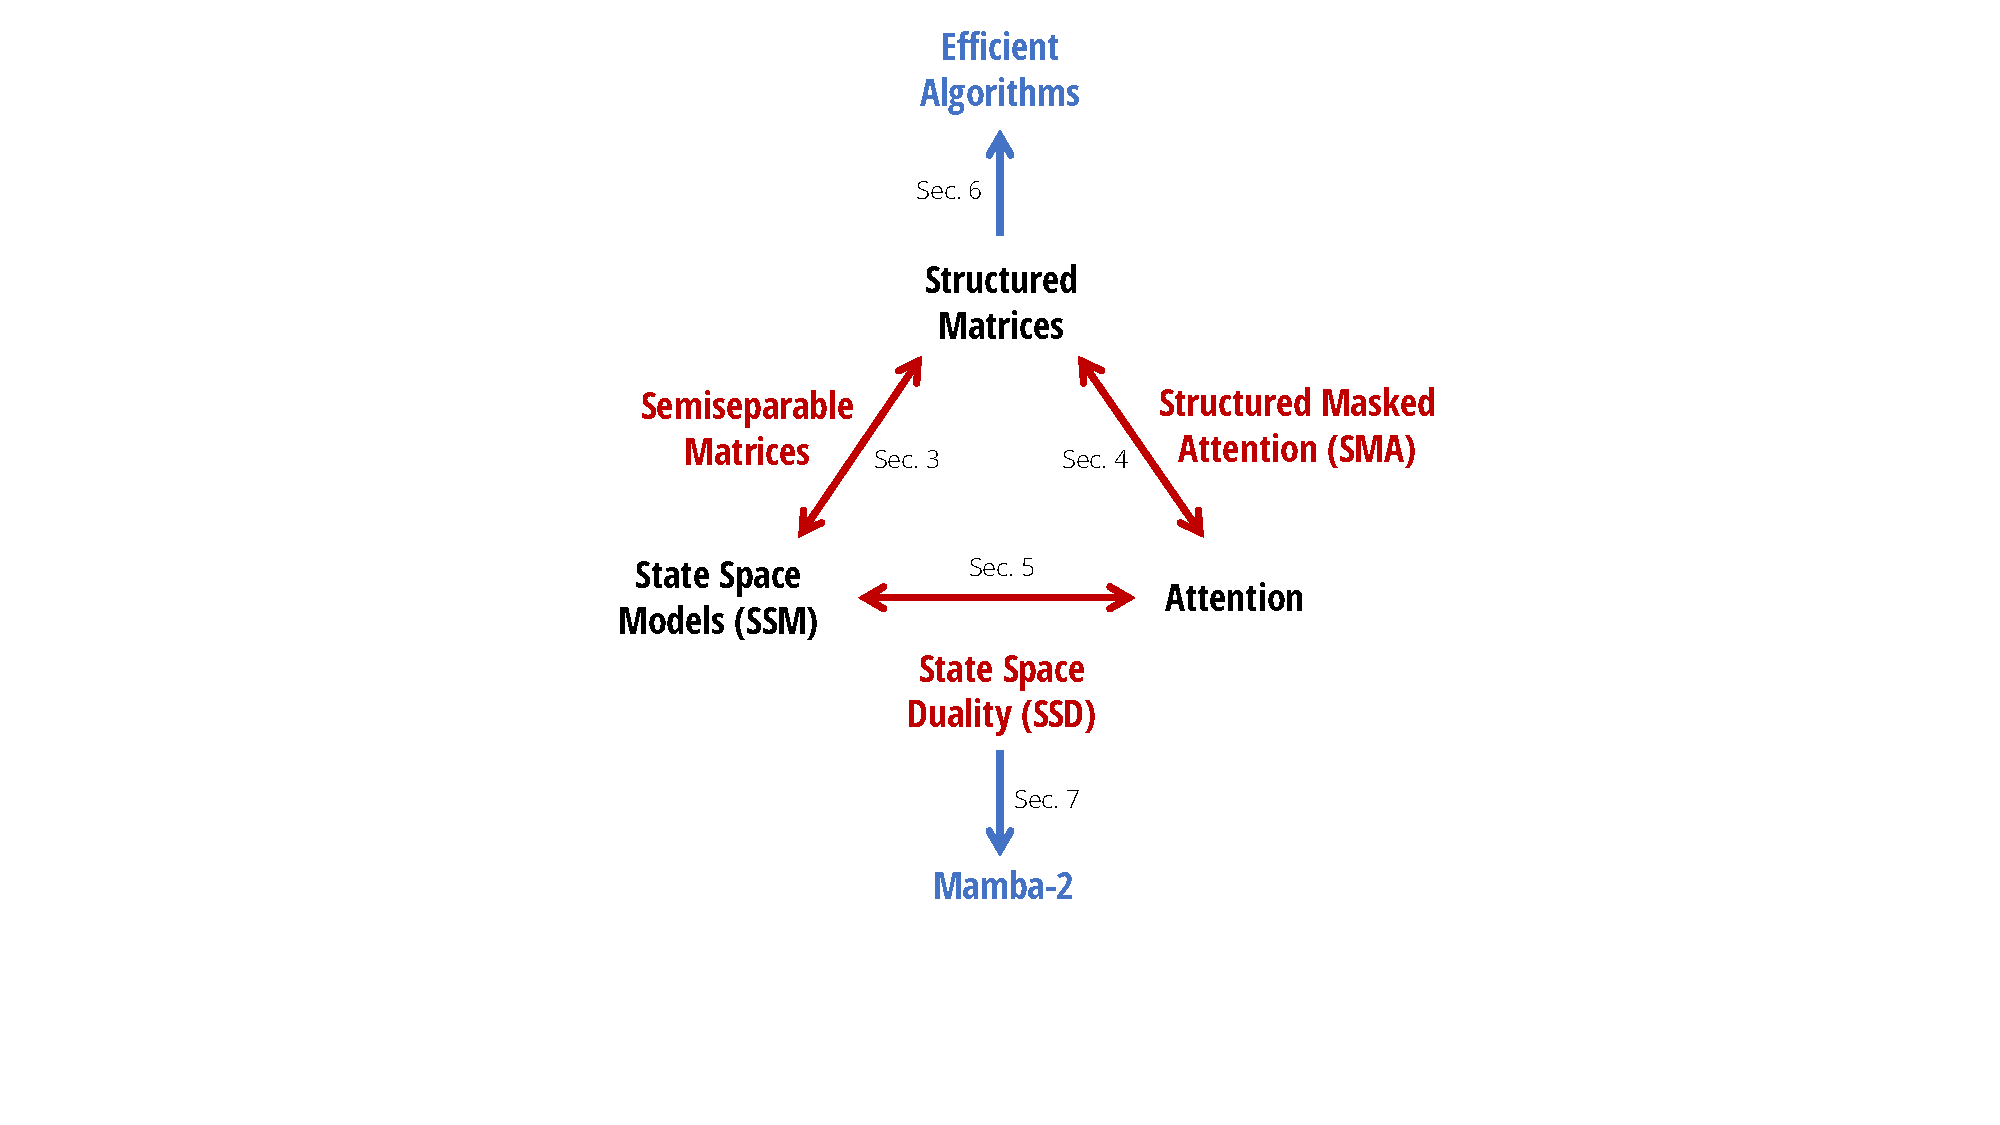
\includegraphics[width=\linewidth]{fig/ssd_roadmap.pdf}
  \end{center}
  \caption{
    (\textbf{Structured State-Space Duality}.)
    This paper fleshes out the relationship between state space models and attention through the bridge of structured matrices.
  }
  \label{fig:roadmap}
\end{wrapfigure}
}{}

\para{State Space Duality.}
Our framework connecting structured SSMs and variants of attention, which we call \textbf{structured state space duality} (SSD),
is made through the abstractions of \textbf{structured matrices}:
matrices with subquadratic parameters and multiplication complexity.
We develop two broad frameworks for representing sequence models, one as matrix transformations and one as tensor contractions, which each reveal different perspectives of the duality.
Our technical contributions include:
\begin{itemize}[leftmargin=*,itemsep=0pt,topsep=0pt]
  \item We show an equivalence between state space models and a well-studied family of structured matrices called \textbf{semiseparable matrices}\iftoggle{arxiv}{ (\cref{sec:ssm})}{}.
    This connection is at the heart our framework, revealing new properties and algorithms for SSMs. A central message of this paper is that \emph{different methods of computing state space models can be reframed as various matrix multiplication algorithms on structured matrices}.
  \item We significantly improve the theory of linear attention~\citep{katharopoulos2020transformers}.
    We first provide an incisive proof of its recurrent form through the language of tensor contractions, and then generalize it to a new family of \textbf{structured masked attention (SMA)}\iftoggle{arxiv}{ (\cref{sec:attention})}{}.
  \item We connect SSMs and SMA, showing that they have a large intersection that are duals of each other, possessing both SSM-like linear and attention-like quadratic forms\iftoggle{arxiv}{ (\cref{sec:ssd})}{}.
    \iftoggle{arxiv}{We also prove that any kernel attention method possessing a fast recurrent form must be an SSM.}{}
\end{itemize}


Beyond its intrinsic theoretical value, our framework opens up a broad set of directions for understanding and improving sequence models.

\para{Efficient Algorithms.}
First and most importantly, our framework exposes new efficient and easily-implementable algorithms for computing SSMs\iftoggle{arxiv}{ (\cref{sec:efficient})}{}.
We introduce a new \textbf{SSD algorithm}, based on block decompositions of semiseparable matrices, that takes advantage of both the linear SSM recurrence and quadratic dual form, obtaining optimal tradeoffs on all main efficiency axes (e.g. training and inference compute, memory usage, and ability to leverage matrix multiplication units on modern hardware).
A dedicated implementation of SSD is $2-8\times$ faster than the optimized selective scan implementation of Mamba, while simultaneously allowing for much larger recurrent state sizes ($8\times$ the size of Mamba or even higher, with minimal slowdown).
SSD is highly competitive with optimized implementations of softmax attention (FlashAttention-2~\citep{dao2023flashattention2}), crossing over at sequence length 2K and 6$\times$ faster at sequence length 16K.


\iftoggle{arxiv}{
\para{Architecture Design.}
One major obstacle to adopting new architectures such as SSMs is the ecosystem tailored to Transformers, such as hardware-efficient optimization and parallelism techniques for large-scale training.
Our framework allows using established conventions and techniques for attention to build a vocabulary of architecture design choices for SSMs, and further improve them (\cref{sec:architecture}).
For example, we introduce the analog of heads from multi-head attention (MHA) to SSMs.
We show that the Mamba architecture is a \textbf{multi-input SSM (MIS)} that turns out to be analogous to \textbf{multi-value attention (MVA)}, and compare other variants of Mamba with different head structures.

We also use these ideas to make slight modifications to the Mamba block, which allows tensor parallelism to be implemented (e.g. in the style of Megatron~\citep{shoeybi2019megatron}).
The main ideas include introducing grouped-value attention (GVA) head structure, and moving all data-dependent projections to occur in parallel at the beginning of the block.


}{
  \para{Mamba-2.}
  Additionally, inspired by the connection between SSMs and Transformers, we slightly modify the neural network architecture of Mamba by moving all data-dependent projections to occur in parallel at the beginning of the block. %
}
The combination of the modified parallel Mamba block, together with using SSD as the inner SSM layer, results in the \textbf{Mamba-2} architecture.
We investigate Chinchilla scaling laws for Mamba-2 in the same setting as Mamba, finding that it Pareto dominates Mamba and Transformer++ in both perplexity and wall-clock time.
We additionally train a family of Mamba-2 models at varying sizes on the Pile, showing that it matches or outperforms Mamba and open source Transformers on standard downstream evaluations.
For example, Mamba-2 with 2.7B parameters trained on 300B tokens on the Pile outperforms Mamba-2.8B, Pythia-2.8B and even Pythia-6.9B trained on the same dataset.

\iftoggle{arxiv}{
\paragraph{Systems Optimizations.}
The SSD framework connects SSMs and Transformers, allowing us to leverage a rich body of work on systems optimizations developed for Transformers~(\cref{sec:systems}).
\begin{itemize}[leftmargin=*,itemsep=0pt,topsep=0pt]
  \item For example, Tensor Parallelism (TP) is an important model parallelism technique to train large Transformer models by splitting each layer across GPUs on the same node.
    We design Mamba-2 to be TP-friendly, reducing the number of synchronization point per block by half.
  \item For very long sequences whose activations do not fit on one device, sequence parallelism has been developed for the attention blocks.
    We describe how to train SSMs in general and Mamba-2 in particular with sequence parallelism, by passing the recurrent states between devices.
  \item For finetuning with examples of different lengths, for best efficiency, Transformer requires sophisticated techniques to remove padding tokens and perform attention on variable length sequences.
    We show how Mamba-2 can be trained with variable sequence lengths efficiently, requiring no padding tokens.
\end{itemize}
}{}

\cref{sec:experiments} empirically validates Mamba-2 on language modeling, training efficiency, and a difficult multi-query associative recall task~\citep{arora2024simple}.
Finally, in \cref{sec:related}, we provide an extended related work and discuss potential research directions opened up by our framework.

Model code and pre-trained checkpoints are open-sourced at \url{https://github.com/state-spaces/mamba}.






\section{Methodology}
\ours follows the same framework as speculative decoding, where each decoding step primarily consists of three substeps: (1) generating candidates, (2) processing candidates, and (3) accepting candidates. For \ours, (1) is achieved by \ours heads, (2) is realized by tree attention, and since \ours heads are on top of the original model, the logits calculated in (2) can be used for substep (1) for the next decoding step. The final step (3) can be realized by either rejection sampling~\citep{leviathan2022fast,chen2023accelerating} or typical acceptance (Section~\ref{sec:typical_acceptance}). The overall pipeline is illustrated in Figure~\ref{fig:pipeline}.

In this section, we first introduce the key components of \ours, including \ours heads, and tree attention. Then, we present two levels of fine-tuning procedures for \ours to meet the needs of different use cases. Finally, we propose two extensions to \ours, including self-distillation and typical acceptance, to handle situations where no training data is available for \ours and to improve the efficiency of the decoding process, respectively.
\subsection{Key Components}
\subsubsection{\ours Heads}
\label{sec:medusa_heads}
In speculative decoding, subsequent tokens are predicted by an auxiliary draft model. This draft model must be small yet effective enough to generate continuations that the original model will accept. Fulfilling these requirements is a challenging task, and existing approaches~\citep{spector2023accelerating,miao2023specinfer} often resort to separately \emph{pre-training} a smaller model. This pre-training process demands substantial additional computational resources. For example, in \citep{miao2023specinfer}, a reported 275 NVIDIA A100 GPU hours were used. Additionally, separate pre-training can potentially create a distribution shift between the draft model and the original model, leading to continuations that the original model may not favor. \citet{chen2023accelerating} have also highlighted the complexities of serving multiple models in a distributed environment.

\textcolor{black}{To streamline and democratize the acceleration of LLM inference, we take inspiration from \citet{stern2018blockwise}, which utilizes parallel decoding for tasks such as machine translation and image super-resolution. \ours heads}
 are additional decoding heads appended to the last hidden states of the original model. Specifically, given the original model's last hidden states $h_t$ at position $t$, we add $K$ decoding heads to $h_t$. The $k$-th head is used to predict the token in the $(t+k+1)$-th position of the next tokens (the original language model head is used to predict the $(t+1)$-th position). The prediction of the $k$-th head is denoted as $p_t^{(k)}$, representing a distribution over the vocabulary, while the prediction of the original model is denoted as $p_t^{(0)}$. Following the approach of \citet{stern2018blockwise}, we utilize a single layer of feed-forward network with a residual connection for each head. We find that this simple design is sufficient to achieve satisfactory performance. The definition of the $k$-th head is outlined as:

\begin{align*}
p_t^{(k)} = \text{softmax}\left(W_2^{(k)} \cdot \left(\text{SiLU}(W_1^{(k)} \cdot h_t)+h_t\right)\right),\\
\text{where } W_2^{(k)}\in\mathbb{R}^{d\times V}, W_1^{(k)}\in\mathbb{R}^{d\times d}.
\end{align*}

\textcolor{black}{$d$ is the output dimension of the LLM's last hidden layer and $V$ is the vocabulary size.}
\textcolor{black}{We initialize $W_2^{(k)}$ identically to the original language model head, and $W_1^{(k)}$ to zero.}
This aligns the initial prediction of \ours heads with that of the original model. The SiLU activation function~\citep{elfwing2017sigmoidweighted} is employed following the Llama models~\citep{touvron2023llama}.

Unlike a draft model, \ours heads are trained in conjunction with the original backbone model, which can remain \emph{frozen} during training (\ours-1) or be trained together (\ours-2). This method allows for fine-tuning large models even on a single GPU, taking advantage of the powerful base model's learned representations. Furthermore, it ensures that the distribution of the \ours heads aligns with that of the original model, thereby mitigating the distribution shift problem. Additionally, since the new heads consist of just a single layer akin to the original language model head, \ours does not add complexity to the serving system design and is friendly to distributed settings. We will discuss the training recipe for \ours heads in Section~\ref{sec:training_recipe}.

\subsubsection{Tree Attention}
\label{sec:tree_attention}
Through \ours heads, we obtain probability predictions for the subsequent $K+1$ tokens. These predictions enable us to create length-$K+1$ continuations as candidates. While the speculative decoding studies~\citep{leviathan2022fast,chen2023accelerating} suggest sampling a single continuation as the candidate, leveraging multiple candidates during decoding can enhance the expected acceptance length within a decoding step. Nevertheless, more candidates can also raise computational demands. To strike a balance, we employ a tree-structured attention mechanism to process multiple candidates concurrently.
\begin{figure}[ht]
    \centering
    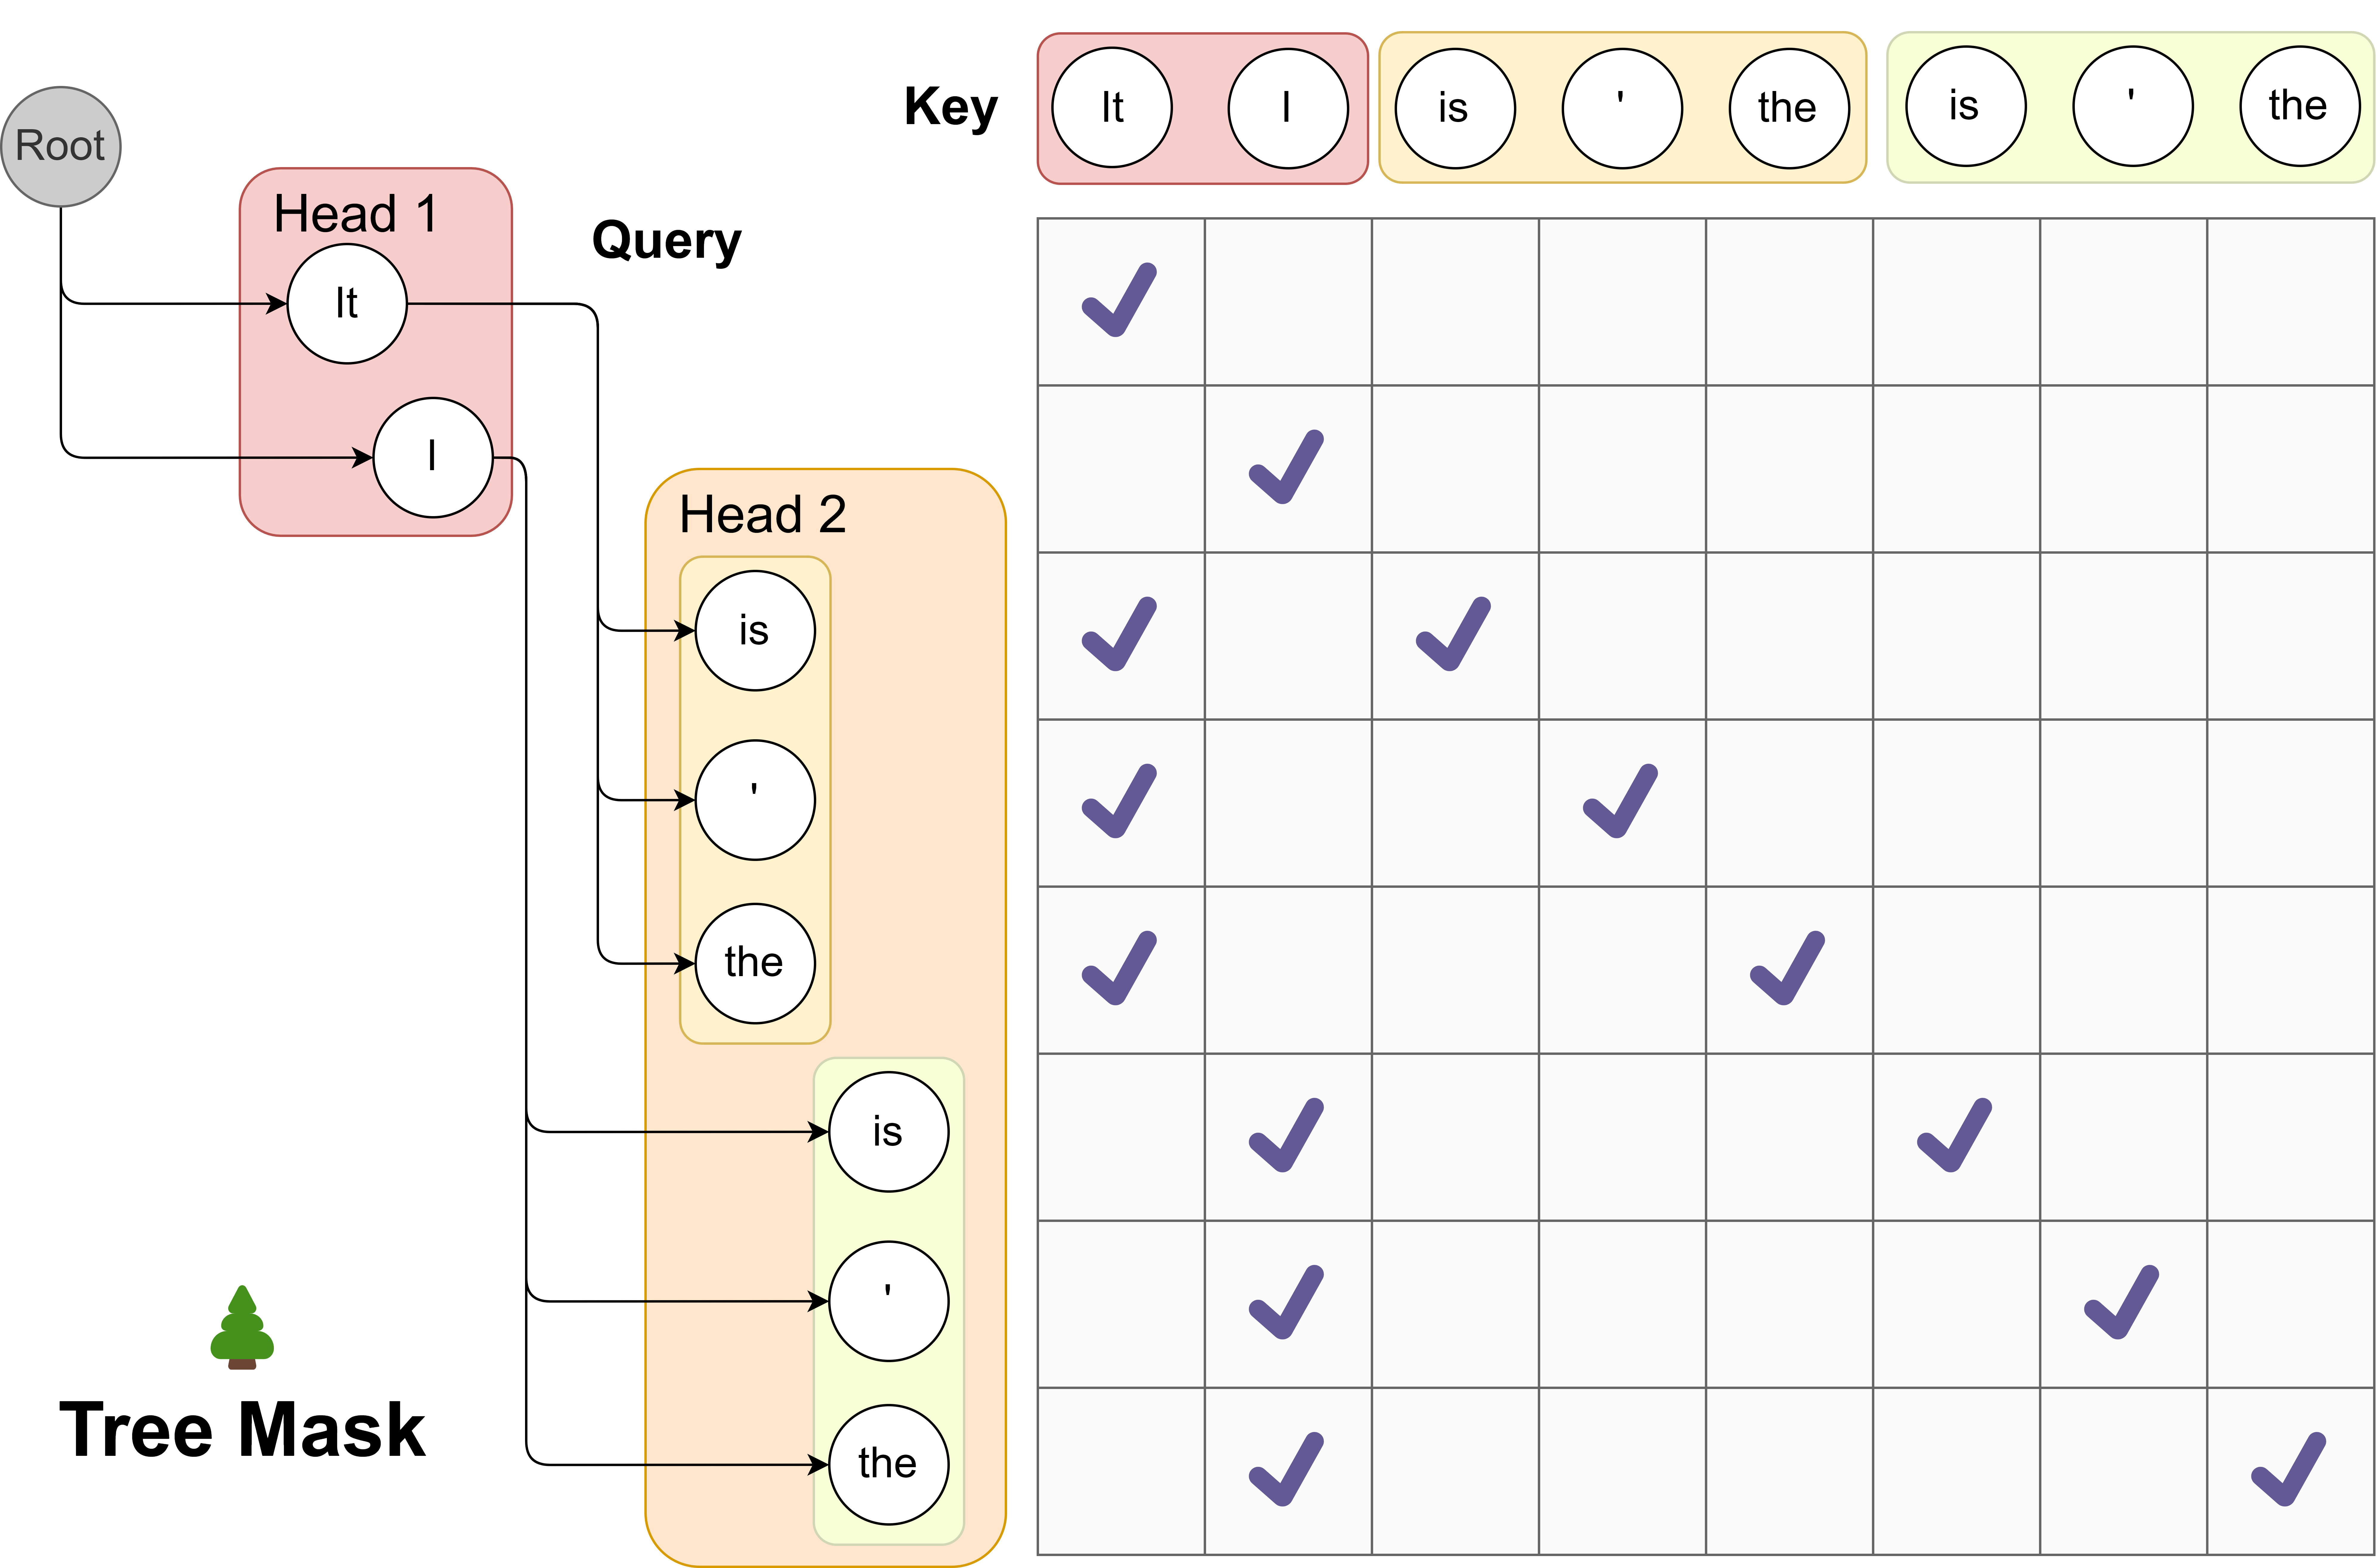
\includegraphics[width=0.45\textwidth]{tree_attention.png}
    \caption{
    We demonstrates the use of tree attention to process multiple candidates concurrently. As exemplified, the top-2 predictions from the first \ours head and the top-3 from the second result in a total of $2\times3=6$ candidates. Each of these candidates corresponds to a distinct branch within the tree structure. To guarantee that each token only accesses its predecessors, we devise an attention mask that exclusively permits attention flow from the current token back to its antecedent tokens. The positional indices for positional encoding are adjusted in line with this structure.}
    \label{fig:tree_attention}
\end{figure}
This attention mechanism diverges from the traditional causal attention paradigm. Within this framework, only tokens from the same continuation are regarded as historical data. Drawing inspiration from the concept of embedding graph structures into attention as proposed in the graph neural network domain~\citep{ying2021transformers}, we incorporate the tree structure into our attention mask, visualized in Figure~\ref{fig:tree_attention}. Remarkably, similar ideas have also been explored in independent works like \citet{miao2023specinfer,spector2023accelerating}, where they follow a bottom-up approach and construct the tree by merging multiple candidates generated by a draft model. In our method, we instead take a top-down approach to build the tree thanks to the structure of candidates generated by \ours heads. For a given $k$-th head, its top-$s_k$ predictions serve as the basis for candidate formation, where $s_k$ is a designated hyperparameter. These candidates are established by determining the Cartesian product of the top-$s_k$ predictions from each head. For instance, in Figure~\ref{fig:tree_attention}, with $s_1=2$ and $s_2=3$, each first head prediction can be succeeded by any prediction from the second head. This leads to a tree structure where $s_k$ branches exist at the $k$-th level (considering a virtual root as the $0$-level, in practice, this $0$-level is for the prediction of the language model head of the original model, which can be sampled independently). Within this tree, only a token's predecessors are seen as historical context, and our attention mask ensures that the attention is only applied on a token's predecessors. By employing this mask and properly setting the positional indices for positional encoding, we can process numerous candidates simultaneously without the need to expand the batch size. The cumulative number of new tokens is calculated as $\sum_{k=1}^K \prod_{i=1}^k s_i$.

In this section, we demonstrate the most simple and regular way to construct the tree structure by taking the Cartesian product. However, it is possible to construct the tree structure in a more sophisticated way and exploit the unbalanced accuracy of different top predictions of different heads. We will discuss this in Section~\ref{sec:optimized_tree_construction}.
\subsection{Training Strategies}
\label{sec:training_recipe}
At the most basic level, we can train \ours heads by freezing the backbone model and fine-tuning \ours heads. However, training the backbone in conjunction with the \ours heads can significantly enhance the accuracy of the \ours heads. Depending on the computational resources and the specific reqirements of the use case, we propose two levels of training strategies for \ours heads.

In this section, we assume the availability of a training dataset that aligns with the target model’s output distribution. This could be the dataset used for Supervised Fine-Tuning (SFT) of the target model. We will discuss eliminating the need for such a dataset using a self-distillation approach in Section~\ref{sec:self_distillation}.
\subsubsection{\ours-1: Frozen Backbone}
\label{sec:frozen_backbone}
To train \ours heads with a frozen backbone model, we can use the cross-entropy loss between the prediction of \ours heads and the ground truth. Specifically, given the ground truth token $y_{t+k+1}$ at position $t+k+1$, the loss for the $k$-th head is $\mathcal{L}_k = -\log p_t^{(k)}(y_{t+k+1})$ where $p_t^{(k)}(y)$ denotes the probability of token $y$ predicted by the $k$-th head. We also observe that $\mathcal{L}_k$ is larger when $k$ is larger, which is reasonable since the prediction of the $k$-th head is more uncertain when $k$ is larger. Therefore, we can add a weight $\lambda_k$ to $\mathcal{L}_k$ to balance the loss of different heads. And the total \ours loss is:
\begin{align}
    \label{eq:loss_medusa_1}
    \mathcal{L}_{\text{\ours-1}} = \sum_{k=1}^K -\lambda_k\log p_t^{(k)}(y_{t+k+1}).
\end{align}

In practice, we set $\lambda_k$ as the $k$-th power of a constant like $0.8$. Since we only use the backbone model for providing the hidden states, we can use a quantized version of the backbone model to reduce the memory consumption. This introduces a more democratized way to accelerate LLM inference, as with the quantization, \ours can be trained for a large model on a single consumer GPU similar to QLoRA~\citep{dettmers2023qlora}. The training only takes a few hours (e.g., 5 hours for \ours-1 on Vicuna 7B model with a single NVIDIA A100 PCIE GPU to train on 60k ShareGPT samples).
\subsubsection{\ours-2: Joint Training}
\label{sec:joint_training}
To further improve the accuracy of \ours heads, we can train \ours heads together with the backbone model. However, this requires a special training recipe to preserve the backbone model's next-token prediction capability and output quality. To achieve this, we propose three strategies:
\begin{itemize}
    \item \textbf{Combined loss}: To keep the backbone model's next-token prediction capability, we need to add the cross-entropy loss of the backbone model $\mathcal{L}_{\text{LM}}=-\log p_t^{(0)}(y_{t+1})$ to the \ours loss. We also add a weight $\lambda_0$ to balance the loss of the backbone model and the \ours heads. Therefore, the total loss is:
    \begin{align}
        \label{eq:loss_medusa_2}
        \mathcal{L}_{\text{\ours-2}} = \mathcal{L}_{\text{LM}} + \lambda_0\mathcal{L}_{\text{\ours-1}}.
    \end{align}
    \item \textbf{Differential learning rates}: Since the backbone model is already well-trained and the \ours heads need more training, we can use separate learning rates for them to enable faster convergence of \ours heads while preserving the backbone model's capability.
    \item \textbf{Heads warmup}: Noticing that at the beginning of training, the \ours heads have a large loss, which leads to a large gradient and may distort the backbone model's parameters. Following the idea from \citet{kumar2022finetuning}, we can employ a two-stage training process. In the first stage, we only train the \ours heads as \ours-1. In the second stage, we train the backbone model and \ours heads together with a warmup strategy. Specifically, we first train the backbone model for a few epochs, then train the \ours heads together with the backbone model. Besides this simple strategy, we can also use a more sophisticated warmup strategy by gradually increasing the weight $\lambda_0$ of the backbone model's loss. We find both strategies work well in practice.
\end{itemize}
Putting these strategies together, we can train \ours heads together with the backbone model without hurting the backbone model's capability. Moreover, this recipe can be applied together with Supervised Fine-Tuning (SFT), enabling us to get a model with native \ours support.
\subsubsection{How to Select the Number of Heads}
Empirically, we found that five heads are sufficient at most. Therefore, we recommend training with five heads and referring to the strategy described in Section~\ref{sec:optimized_tree_construction} to determine the optimal configuration of the tree attention. With optimized tree attention, sometimes three or four heads may be enough for inference. In this case, we can ignore the redundant heads without overhead.

\subsection{Extensions}
\subsubsection{Typical Acceptance}
\label{sec:typical_acceptance}
In speculative decoding papers~\citep{leviathan2022fast,chen2023accelerating}, authors employ rejection sampling to yield diverse outputs that align with the distribution of the original model. However, subsequent implementations~\citep{gante2023assisted,spector2023accelerating} reveal that this sampling strategy results in diminished efficiency as the sampling temperature increases. Intuitively, this can be comprehended in the extreme instance where the draft model is the same as the original one\textcolor{black}{:} 
Using greedy decoding, all output of the draft model will be accepted, therefore maximizing the efficiency. 
Conversely, rejection sampling introduces extra overhead, as the draft model and the original model are sampled independently. Even if their distributions align perfectly, the output of the draft model may still be rejected.

However, in real-world scenarios, sampling from language models is often employed to generate diverse responses, and the temperature parameter is used merely to modulate the ``creativity'' of the response. Therefore, higher temperatures should result in more opportunities for the original model to accept the draft model's output. We ascertain that it is typically unnecessary to match the distribution of the original model. Thus, we propose employing a \emph{typical acceptance} scheme to select plausible candidates rather than using rejection sampling. This approach draws inspiration from truncation sampling studies~\citep{hewitt2022truncation} (refer to \textcolor{black}{Appendix}~\ref{sec:related_work} for an in-depth explanation). Our objective is to choose candidates that are \emph{typical}, meaning they are not exceedingly improbable to be produced by the original model. We use the prediction probability from the \emph{original model} as a natural gauge for this and establish a threshold based on the prediction distribution to determine acceptance. Specifically, given $x_1, x_2, \cdots, x_n$ as context, when evaluating the candidate sequence \textcolor{black}{$(x_{n+1}, x_{n+2}, \cdots, x_{n+K+1})$ }(composed by top predictions of the original language model head and \ours heads), we consider the condition
\begin{align*}
p_{\text{original}}(x_{n+k}|x_1, x_2, \cdots, x_{n+k-1}) > \\\min\rbr{\epsilon, \delta\exp\rbr{-H(p_{\text{original}}(\cdot|x_1, x_2, \cdots, x_{n+k-1}))}},
\end{align*}
where $H(\cdot)$ denotes the entropy function, and $\epsilon, \delta$ are \textcolor{black}{the hard threshold and the entropy-dependent
threshold respectively}. This criterion is adapted from \citet{hewitt2022truncation} and rests on two observations: (1) tokens with relatively high probability are meaningful, and (2) when the distribution's entropy is high, various continuations may be deemed reasonable. During decoding, every candidate is evaluated using this criterion, and a \emph{prefix} of the candidate is accepted if it satisfies the condition. To guarantee the generation of at least one token at each step, we apply \emph{greedy decoding} for the first token and \emph{unconditionally} accept it while employing typical acceptance for subsequent tokens. The final prediction for the current step is determined by the \emph{longest accepted prefix} among all candidates.

Examining this scheme leads to several insights. Firstly, when the temperature is set to $0$, it reverts to greedy decoding, as only the most probable token possesses non-zero probability. As the temperature surpasses $0$, the outcome of greedy decoding will consistently be accepted with appropriate $\epsilon, \delta$, since those tokens have the maximum probability, yielding maximal speedup. Likewise, in general scenarios, an increased temperature will correspondingly result in longer accepted sequences, as corroborated by our experimental findings.

Empirically, we verify that typical acceptance can achieve a better speedup while maintaining a similar \textcolor{black}{generation quality} as shown in Figure~\ref{fig:threshold_ablation}.
\subsubsection{Self-Distillation}
\label{sec:self_distillation}
In Section~\ref{sec:training_recipe}, we assume the existence of a training dataset that matches the target model's output distribution. However, this is not always the case. For example, the model owners may only release the model without the training data, or the model may have gone through a Reinforcement Learning with Human Feedback (RLHF) procedure, which makes the output distribution of the model different from the training dataset. To tackle this issue, we propose an automated self-distillation pipeline to use the model itself to generate the training dataset for \ours heads, which matches the output distribution of the model.

The dataset generation process is straightforward. We first take a public seed dataset from a domain similar to the target model; for example, using the ShareGPT~\citep{sharegpt2023} dataset for chat models. Then, we simply take the prompts from the dataset and ask the model to reply to the prompts. In order to obtain multi-turn conversation samples, we can sequentially feed the prompts from the seed dataset to the model. Or, for models like Zephyr 7B~\citep{tunstall2023zephyr}, which are trained on both roles of the conversation, they have the ability to self-talk, and we can simply feed the first prompt and let the model generate multiple rounds of conversation.

For \ours-1, this dataset is sufficient for training \ours heads. However, for \ours-2, we observe that solely using this dataset for training the backbone and \ours heads usually leads to a lower generation quality. In fact, even without training \ours heads, training the backbone model with this dataset will lead to performance degradation. This suggests that we also need to use the original model's probability prediction instead of using the ground truth token as the label for the backbone model, similar to classic knowledge distillation works~\citep{kim2016sequencelevel}. Concretely, the loss for the backbone model is:
\begin{align*}
    \mathcal{L}_{\text{LM-distill}} = KL(p_{\text{original},t}^{(0)}||p_t^{(0)}),
\end{align*}
where $p_{\text{original},t}^{(0)}$ denotes the probability distribution of the original model's prediction at position $t$.

However, naively, to obtain the original model's probability prediction, we need to maintain two models during training, increasing the memory requirements. To further alleviate this issue, we propose a simple yet effective way to exploit the self-distillation setup. We can use a parameter-efficient adapter like LoRA~\citep{hu2021lora} for fine-tuning the backbone model. In this way, the original model is simply the model with the adapter turned off. Therefore, the distillation does not require additional memory consumption. Together, this self-distillation pipeline can be used to train \ours-2 without hurting the backbone model's capability and introduce almost no additional memory consumption. Lastly, one tip about using self-distillation is that it is preferable to use LoRA without quantization in this case, otherwise, the teacher model will be the quantized model, which may lead to a lower generation quality.

\subsubsection{Searching for the Optimized Tree Construction}
\label{sec:optimized_tree_construction}
In Section~\ref{sec:tree_attention}, we present the simplest way to construct the tree structure by taking the Cartesian product. However, with a fixed budget for the number of total nodes in the tree, a regular tree structure may not be the best choice. Intuitively, those candidates composed of the top predictions of different heads may have different accuracies. Therefore, we can leverage an estimation of the accuracy to construct the tree structure.

Specifically, we can use a calibration dataset and calculate the accuracies of the top predictions of different heads. Let $a_k^{(i)}$ denote the accuracy of the $i$-th top prediction of the $k$-th head\footnote{Here, the accuracy is defined for the single top $i$-th token, i.e., this accuracy is equal to top-$i$ accuracy minus top-$(i-1)$ accuracy.}. Assuming the accuracies are independent, we can estimate the accuracy of a candidate sequence composed by the top $\sbr{i_1, i_2, \cdots, i_k}$ predictions of different heads as $\prod_{j=1}^k a_j^{(i_j)}$. Let $I$ denote the set of all possible combinations of $\sbr{i_1, i_2, \cdots, i_k}$ and each element of $I$ can be mapped to a node of the tree (not only leaf nodes but all nodes are included). Then, the expectation of the acceptance length of a candidate sequence is:
\begin{align*}
    \sum_{\sbr{i_1, i_2, \cdots, i_k}\in I}\prod_{j=1}^k a_j^{(i_j)}.
\end{align*}
Thinking about building a tree by adding nodes one by one, the contribution of a new node to the expectation is exactly the accuracy associated with the node. Therefore, we can greedily add nodes to the tree by choosing the node that is connected to the current tree and has the highest accuracy. This process can be repeated until the total number of nodes reaches the desired number. In this way, we can construct a tree that maximizes the expectation of the acceptance length. Further details can be found in Appendix~\ref{appendix:sparse_tree}.


\vspace{-0.2cm}
\section{Experiments Details}
\label{sec:exp}

\vspace{-0.2cm}
\subsection{Roadmap Insights on FFHQ-256\texorpdfstring{~\cite{sg1}}{}}
\label{sub:arc-experiments}
\vspace{-0.1cm}
As per Table~\ref{tab:roadmap}, Config A (vanilla StyleGAN2) achieves an FID of 7.52 using the official implementation on FFHQ-256. Config B with all tricks removed achieves an FID of 12.46---performance drops as expected. 
Config C, with a well-behaved loss, achieves an FID of 11.65. But, now training is sufficiently stable to improve the architecture.

Config D, which improves $G$ and $D$ based on the classic ResNet and ConvNeXt findings, achieves an FID of 9.95. The output skips of the StyleGAN2 generator are no longer useful given our new architecture; including them produces a worse FID of 10.17. Karras~\etal find that the benefit of output skips is mostly related to gradient magnitude dynamics~\cite{sg3}, and this has been addressed by our ResNet architecture. For StyleGAN2, Karras~\etal conclude that a ResNet architecture is harmful to $G$~\cite{sg2}, but this is not true in our case as their ResNet implementation is considerably different from ours: 1) Karras~\etal use one 3-3 residual block for each resolution stage, while we have a separate transition layer and two 1-3-1 residual blocks; 2) i.3) and i.4) are violated as they do not have a linear residual block~\cite{mobnet} and the transition layer is placed on the skip branch of the residual block rather than the stem; 3) the essential principle of ResNet~\cite{resnet}---identity mapping~\cite{resnet2}---is violated as Karras~\etal divide the output of the residual block by $\sqrt{2}$ to avoid variance explosion due to the absence of a proper initialization scheme.

For Config E, we conduct two experiments that ablate i.\ref{item:i1} (increased width with depthwise conv.) and i.\ref{item:i2} (an inverted bottleneck). We add GroupedConv and reduce the bottleneck compression ratio to two given the same model size. Each bottleneck is now 1.5$\times$ the width of Config A, and the FID drops to 7.51, surpassing the performance of StyleGAN2. By inverting the stem and the bottleneck dimensions to enhance the capacity of GroupedConv, our final model achieves an FID of 7.05, exceeding StyleGAN2.


\begin{wraptable}[12]{r}{6.5cm}
\vspace{-1.25cm}
\centering
\caption{StackedMNIST 1000-mode coverage.}
% Our model outperforms other GANs in terms of $D_\text{KL}$, indicating that we are better able to recover the distribution.}
\vspace{-0.4cm}
\resizebox{0.8\linewidth}{!}{
\begin{tblr}{
  cell{2}{2} = {c},
  cell{2}{3} = {c},
  cell{3}{2} = {c},
  cell{3}{3} = {c},
  cell{4}{2} = {c},
  cell{4}{3} = {c},
  cell{5}{2} = {c},
  cell{5}{3} = {c},
  cell{6}{2} = {c},
  cell{6}{3} = {c},
  cell{7}{2} = {c},
  cell{7}{3} = {c},
  cell{8}{2} = {c},
  cell{8}{3} = {c},
  cell{9}{2} = {c},
  cell{9}{3} = {c},
  cell{10}{2} = {c},
  cell{10}{3} = {c},
  cell{11}{2} = {c},
  cell{11}{3} = {c},
  cell{12}{2} = {c},
  cell{12}{3} = {c},
  hline{2,12} = {1-3}{},
}
Model     & \# modes$\uparrow$ & $D_\text{KL}$$\downarrow$            &  \\
DCGAN~\cite{dcgan}     & 99            & 3.40\phantom{0}&  \\
VEEGAN~\cite{srivastava2017veegan}    & 150           & 2.95\phantom{0}&  \\
WGAN-GP~\cite{wgan-gp}& 959           & 0.73\phantom{0}&  \\
PacGAN~\cite{pacgan}    & 992           & 0.28\phantom{0}&  \\
StyleGAN2~\cite{sg2} & 940           & 0.42\phantom{0}&  \\
PresGAN~\cite{presgan}   & \textbf{1000} & 0.12\phantom{0}&  \\
Adv. DSM~\cite{advsm}  & \textbf{1000} & 1.49\phantom{0}&  \\
VAEBM~\cite{vaebm}     & \textbf{1000} & 0.087          &  \\
DDGAN~\cite{ddgan}     & \textbf{1000} & 0.071          &  \\
MEG~\cite{meg}       & \textbf{1000} & 0.031          &  \\
Ours---Config E     & \textbf{1000} & \textbf{0.029} &  
\end{tblr}
}
\label{tab:stackedmnist}
\end{wraptable}%

\subsection{Mode Recovery --- StackedMNIST\texorpdfstring{~\cite{metz2016unrolled}}{}} 
\vspace{-0.1cm}
We repeat the earlier experiment in 1000-mode convergence on StackedMNIST (unconditional generation), but this time with our updated architecture and with comparisons to SOTA GANs and likelihood-based methods (Tab.~\ref{tab:stackedmnist}, Fig.~\ref{fig:stacked-mnist}). 
One advantage brought up of likelihood-based models such as diffusion over GANs is that they achieve mode coverage~\cite{adm}. We find that most GANs struggle to find all modes. But, PresGAN~\cite{presgan}, DDGAN~\cite{ddgan}, and our approach are successful. Further, our method outperforms all other tested GAN models in term of KL divergence.

\subsection{FID --- FFHQ-256\texorpdfstring{~\cite{sg1}}{} (Optimized)}
\vspace{-0.1cm}
We train Config E model until convergence and with optimized hyperparameters and training schedule on FFHQ at 256$\times$256 (unconditional generation) (Tab.~\ref{tab:ffhq256}, Figs.~\ref{fig:ffhq-256-teaser} and~\ref{fig:ffhq-256}). 
Please see our supplemental material for training details.
%The hyperparameters and schedule are listed in the supplemental material. 
Our model outperforms existing StyleGAN methods, plus four more recent diffusion-based methods. On this common dataset experimental setting, many methods (not listed here) use the bCR~\cite{zhao2021improved} trick---this has only been shown to improve performance on FFHQ-256 (not even at different resolutions of FFHQ)~\cite{zhao2021improved, zhang2022styleswin}. We do not use this trick. 
% no such tricks in our method.
% JT Try to minimize embellishment...
% This is particularly impressive given the fact that the dataset FFHQ was designed for StyleGAN~\cite{sg1} and the StyleGAN series of models were optimized with this specific dataset in mind.
% to achieve this performance.

\subsection{FID --- FFHQ-64\texorpdfstring{~\cite{edm}}{}}
\vspace{-0.1cm}
To compare with EDM~\cite{edm} directly, we evaluate our model on FFHQ at 64$\times$64 resolution. For this, we remove the two highest resolution stages of our 256$\times$256 model, resulting in a generator that is less than half the number of parameters as EDM. Despite this, our model outperforms EDM on this dataset and needs one function evaluation only (Tab.~\ref{tab:ffhq64}).

\begin{figure}
\begin{floatrow}
    %\hspace{-0.75cm}%
    \capbtabbox{%
        \centering
        \resizebox{\linewidth}{!}{
        \begin{tblr}{
          column{2,3} = {r},
          cell{1}{2} = {c},
          cell{1}{3} = {c},
          hline{2,5,9,10} = {-}{},
        }
        Model       & NFE$\downarrow$ & FID$\downarrow$  \\
        StyleGAN2~\cite{sg2}   & 1               & 3.78 \\
        StyleGAN3-T~\cite{sg3} & 1               & 4.81 \\
        StyleGAN3-R~\cite{sg3} & 1               & 3.92 \\
        LDM~\cite{rombach2022high} & 200               & 4.98\\
        ADM (DDIM)~\cite{adm,compdiff} & 500               & 8.41\\
        ADM (DPM-Solver)~\cite{adm,compdiff} & 500               & 8.40\\
        Diffusion Autoencoder~\cite{diffae,compdiff} & 500               & 5.81\\
        Ours---Config E  & 1               & 2.75 \\
        \emph{With ImageNet feature leakage~\cite{kynkaanniemi2022role}:} & & \\
        PolyINR*~\cite{singh2023polynomial} & 1               & 2.72 \\
        StyleGAN-XL*~\cite{sgxl} & 1               & 2.19 \\
        StyleSAN-XL*~\cite{takida2024san} & 1               & 1.68 \\
        \end{tblr}
        }
    }{%
        \caption{
        \label{tab:ffhq256}FFHQ-256. * denotes models that leak ImageNet features.}
    }
    %
    \capbtabbox{%
        \centering
        \resizebox{0.85\linewidth}{!}{
        \begin{tblr}{
          column{2} = {r},
          column{3} = {r},
          hline{2,5,8} = {-}{},
        }
        Model         & NFE$\downarrow$ & FID$\downarrow$ \\
        StyleGAN2~\cite{sg2,anycostgan}     & 1               & 3.32            \\
        MSG-GAN~\cite{karnewar2020msg,anycostgan}       & 1               & 2.7             \\
        Anycost GAN~\cite{anycostgan}   & 1               & 2.52            \\
        VE~\cite{sde,edm}            & 79              & 25.95           \\
        VP~\cite{sde,edm}            & 79              & 3.39            \\
        EDM~\cite{edm}           & 79              & 2.39            \\
        Ours—Config E & 1               & 1.95 \\
        \end{tblr}
        }
    }{%
        \caption{\label{tab:ffhq64}FFHQ-64.}
    }
\end{floatrow}
\vspace{-0.25cm}
\end{figure}


% \begin{figure}
% \begin{floatrow}
%     \capbtabbox{%
%         \centering
%         \resizebox{0.8\linewidth}{!}{
%         \begin{tblr}{
%           column{2,3} = {r},
%           cell{1}{2} = {c},
%           cell{1}{3} = {c},
%           hline{2,9,13} = {-}{},
%         }
%         Model               & NFE$\downarrow$ & FID$\downarrow$ \\
%         BigGAN~\cite{biggan}              & 1               & 14.73 \\
%         TransGAN~\cite{trans}            & 1               & 9.26 \\
%         ViTGAN~\cite{vitgan}              & 1               & 6.66 \\
%         DDGAN~\cite{ddgan}               & 4               & 3.75 \\
%         Diffusion StyleGAN2~\cite{diffusiongan} & 1               & 3.19 \\
%         StyleGAN2 + ADA~\cite{sg2ada}     & 1               & 2.42 \\
%         StyleGAN3-R + ADA~\cite{sg3,studio}   & 1               & 10.83 \\
%         DDPM~\cite{ddpm}               & 1000            & 3.21 \\
%         DDIM~\cite{ddim}                & 50             & 4.67 \\
%         VE~\cite{sde,edm}                  & 35              & 3.11 \\
%         VP~\cite{sde,edm}                  & 35              & 2.48 \\
%         Ours---Config E     & 1               & 1.96 \\
%         \hline
%         \emph{With ImageNet feature leakage~\cite{kynkaanniemi2022role}:} & & \\
%         StyleGAN-XL*~\cite{sgxl}       & 1               & 1.85 \\
%         \end{tblr}
%         }
%     }{%
%         \caption{\label{tab:cifar10}CIFAR-10.}
%     }
%         % \begin{tblr}{
%         %   column{2,3} = {r},
%         %   cell{1}{2}{3} = {},
%         %   hline{2,9,13} = {-}{},
%         % }
%         % Model               & FID$\downarrow$ & Params          \\
%         % BigGAN~\cite{biggan}              & 14.73  & --       \\
%         % TransGAN~\cite{trans}            & 9.26 & --         \\
%         % ViTGAN~\cite{vitgan}              & 6.66 & --         \\
%         % DDGAN~\cite{ddgan}               & 3.75 & --         \\
%         % Diffusion StyleGAN2 & 3.19 & 40.1M           \\
%         % StyleGAN2 + ADA     & 2.42 & 40.1M          \\
%         % StyleGAN3-R + ADA   & 10.83 & 40.1M        \\
%         % DDPM               & 3.21 & 35.2M         \\
%         % DDIM                & 4.67 & --         \\
%         % VE~\cite{edm}                  & 3.11 & 61.8M        \\
%         % VP~\cite{edm}                  & 2.48 & 61.8M         \\
%         % Ours---Config E     & \textbf{1.99}  & 43.0M \\
%         % StyleGAN-XL*~\cite{sgxl}       & 	1.85 & 140.0M \\
%         % \end{tblr}
        
%     %     }
%     % }{%
%     %     \caption{\label{tab:cifar10}CIFAR-10.}
%     % }%
%     %\hspace{-0.75cm}%
%     %\hspace{-0.5cm}%
% \end{floatrow}
% \end{figure}

\subsection{FID --- CIFAR-10~\cite{krizhevsky2009learning}} \vspace{-0.1cm}

\begin{wraptable}[14]{r}{6.5cm}
\vspace{-0.75cm}
\centering
\caption{\label{tab:cifar10}CIFAR-10 performance.}
\vspace{-0.4cm}
\resizebox{0.9\linewidth}{!}{
    \begin{tblr}{
          column{2,3} = {r},
          cell{1}{2} = {c},
          cell{1}{3} = {c},
          hline{2,9,13} = {-}{},
        }
        Model               & NFE$\downarrow$ & FID$\downarrow$ \\
        BigGAN~\cite{biggan}              & 1               & 14.73 \\
        TransGAN~\cite{trans}            & 1               & 9.26 \\
        ViTGAN~\cite{vitgan}              & 1               & 6.66 \\
        DDGAN~\cite{ddgan}               & 4               & 3.75 \\
        Diffusion StyleGAN2~\cite{diffusiongan} & 1               & 3.19 \\
        StyleGAN2 + ADA~\cite{sg2ada}     & 1               & 2.42 \\
        StyleGAN3-R + ADA~\cite{sg3,studio}   & 1               & 10.83 \\
        DDPM~\cite{ddpm}               & 1000            & 3.21 \\
        DDIM~\cite{ddim}                & 50             & 4.67 \\
        VE~\cite{sde,edm}                  & 35              & 3.11 \\
        VP~\cite{sde,edm}                  & 35              & 2.48 \\
        Ours---Config E     & 1               & 1.96 \\
        \hline
        \emph{With ImageNet feature leakage~\cite{kynkaanniemi2022role}:} & & \\
        StyleGAN-XL*~\cite{sgxl}       & 1               & 1.85 \\
        \end{tblr}
}
\end{wraptable}

We train Config E model until convergence and with optimized hyperparameters and training schedule on CIFAR-10 (conditional generation) (Tab.~\ref{tab:cifar10}, Fig.~\ref{fig:cifar10}). Our method outperforms many other GANs by FID even though the model has relatively small capacity. For instance, StyleGAN-XL~\cite{sgxl} has 18\ M parameters in the generator and 125\ M parameters in the discriminator, while our model has a 40\ M parameters between the generator and discriminator combined (Fig.~\ref{fig:fid-50k-vs-params-cifar-10}). Compared to diffusion models like LDM or ADM, GAN inference is significantly cheaper as it requires only one network function evaluation compared to the tens or hundreds of network function evaluations for diffusion models without distillation. 

\begin{wrapfigure}[12]{r}{6.5cm}
    \vspace{-0.4cm}
    \centering
    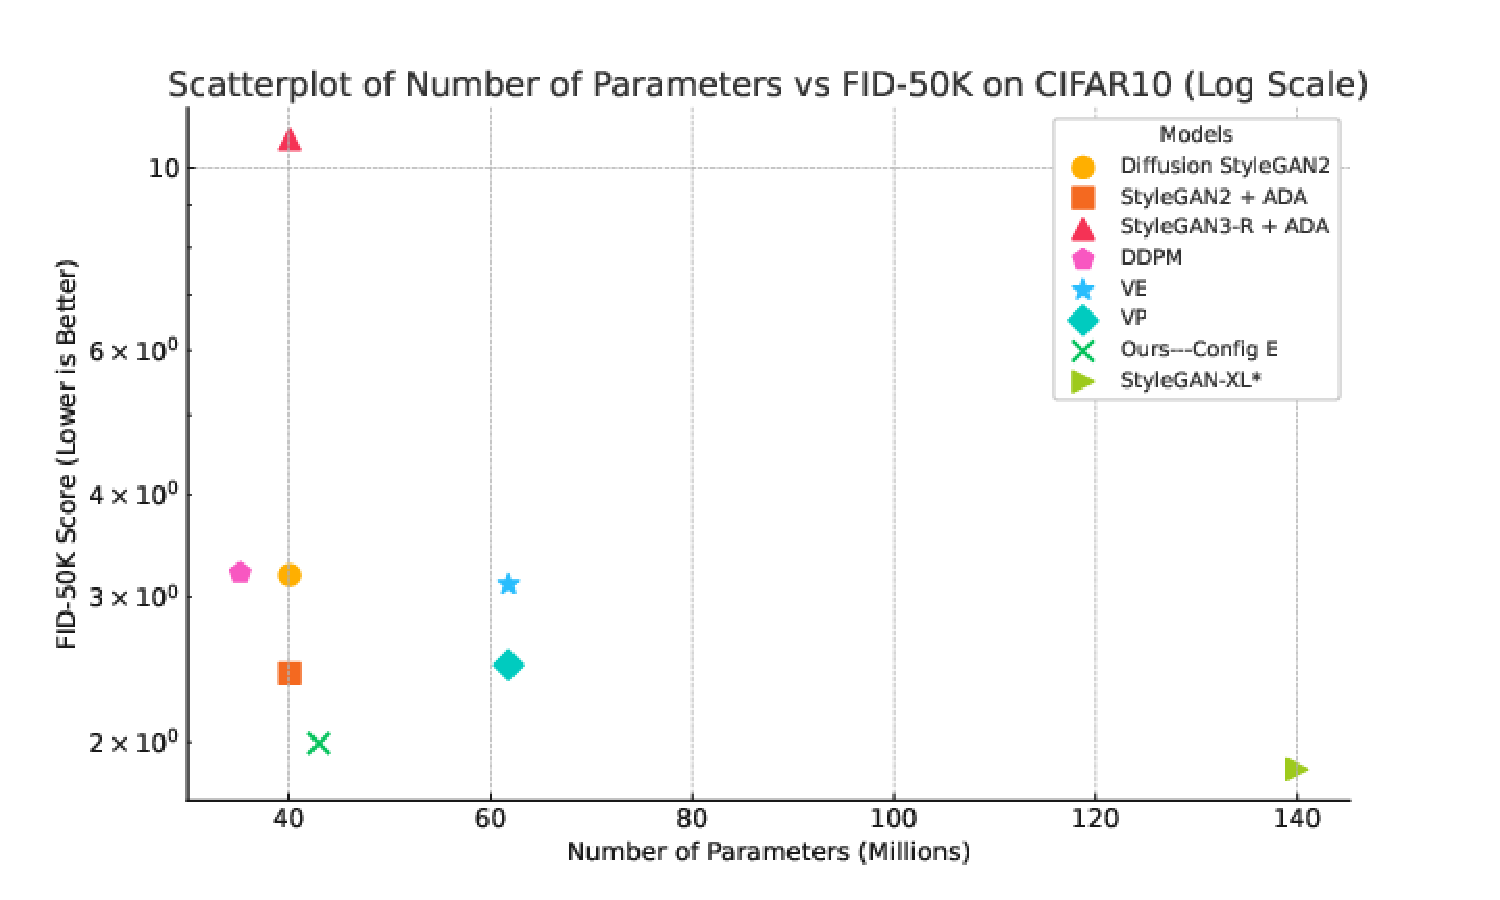
\includegraphics[width=\linewidth,clip,trim={0 0 0 2cm}]{figures/Scatterplot-FID-Parameters-CIFAR10.pdf}
    \caption{Millions of parameters vs.~FID-50K (log scale) on CIFAR-10. Lower is better.}
    \label{fig:fid-50k-vs-params-cifar-10}
\end{wrapfigure}

Many state-of-the-art GANs are derived from Projected GAN~\cite{sauer2021projected}, including StyleGAN-XL~\cite{sgxl} and the concurrent work of StyleSAN-XL~\cite{takida2024san}. These methods use a pre-trained ImageNet classifier in the discriminator. Prior work has shown that a pre-trained ImageNet discriminator can leak ImageNet features into the model~\cite{kynkaanniemi2022role}, causing the model to perform better when evaluating on FID since it relies on a pre-trained ImageNet classifier for the loss. But, this does not improve results in perceptual studies~\cite{kynkaanniemi2022role}. Our model produces its low FID without any ImageNet pre-training.

%\jt{Missing citations here for such methods.}


%\aaron{add NFEs}
%\jt{Which models in our evaluation use this? Any?}

%\jt{What is the second caveat?}

\subsection{FID --- ImageNet-32~\cite{chrabaszcz2017downsampled}}
\label{sec:imagenet32-fid-explain}
We train Config E model until convergence and with optimized hyperparameters and training schedule on ImageNet-32 (conditional generation). We compare against recent GAN models and recent diffusion models in Table~\ref{tab:imagenet32}.
We adjust the number of parameters in the generator of our model to match StyleGAN-XL~\cite{sgxl}'s generator (84M parameters). Specifically, we make the model significantly wider to match. Our method achieves comparable FID despite using a 60\% smaller discriminator (Tab.~\ref{tab:imagenet32}) and despite not using a pre-trained ImageNet classifier.
%, which has been shown to improve FID performance, but not improve results in perceptual studies~\cite{kynkaanniemi2022role}.

\vspace{-0.1cm}
\subsection{FID --- ImageNet-64~\cite{chrabaszcz2017downsampled}}
We evaluate our model on ImageNet-64 to test its scalability. We stack another resolution stage on our ImageNet-32 model, resulting in a generator of 104\ M parameters. This model is nearly 3$\times$ smaller than diffusion-like models~\cite{adm,edm,cm,icm} that rely on the ADM backbone, which contains about 300\ M parameters. Despite the smaller model size and that our model generates samples in one step, it outperforms larger diffusion models with many NFEs on FID (Tab.~\ref{tab:imagenet64}).

\vspace{-0.1cm}
\subsection{Recall}
We evaluate the recall~\cite{precrecall} of our model on each dataset to quantify sample diversity. In general, our model achieves a recall that is similar to or marginally worse than the diffusion model counterpart, yet superior to existing GAN models. For CIFAR-10, the recall of our model peaked at 0.57; as a point of comparison, StyleGAN-XL~\cite{sgxl} has a worse recall of 0.47 despite its lower FID. For FFHQ, we obtain a recall of 0.53 at 64$\times$64 and 0.49 at 256$\times$256, whereas StyleGAN2~\cite{sg2} achieved a recall of 0.43 on FFHQ-256. Our ImageNet-32 model achieved a recall of 0.63; comparable to ADM~\cite{adm}. Our ImageNet-64 model achieved recall 0.59. While this is slightly worse than $\approx$0.63 that many diffusion models achieve, it is better than BigGAN-deep~\cite{biggan} which achieved a recall of 0.48.

\begin{figure}
    \begin{floatrow}
        \capbtabbox{%
        \centering
        \resizebox{0.9\linewidth}{!}{
        \begin{tblr}{
          column{2} = {r},
          column{3} = {r},
          cell{8}{1} = {c=3}{},
          hline{2,7-8} = {-}{},
        }
    Model                                                       & NFE$\downarrow$  & FID$\downarrow$                        \\ 
    DDPM++~\cite{kim2021soft}                  & 1000 & 8.42                                   \\
    VDM~\cite{kingma2021variational}           & 1000 & 7.41                                   \\
    MSGAN~\cite{karnewar2020msg,ning2023input} & 1    & 12.3                                   \\
    ADM~\cite{adm}                             & 1000 & 3.60                                   \\
    DDPM-IP~\cite{ning2023input}               & 1000 & 2.87                                   \\
    Ours—Config E               & 1    & 1.27   \\
    \textit{With ImageNet feature leakage~\cite{kynkaanniemi2022role}:}    \\
    StyleGAN-XL*~\cite{sgxl}                   & 1    & 1.10                                  
    \end{tblr}
        }
    }{%
        \caption{\label{tab:imagenet32}ImageNet-32.}
        % \jt{some are conditional still}}
    }
    %
    \capbtabbox{
        \centering
        \resizebox{0.9\linewidth}{!}{
        \begin{tblr}{
          column{2} = {r},
          column{3} = {r},
          cell{1}{2} = {c},
          cell{1}{3} = {c},
          cell{12}{1} = {c=3}{},
          hline{2-3,11-12} = {-}{},
        }
        Model         & NFE$\downarrow$ & FID$\downarrow$ \\
        BigGAN-deep~\cite{biggan}\phantom{xx}   & 1               & 4.06            \\
        DDPM~\cite{ddpm}          & 250             & 11.0            \\
        DDIM~\cite{ddim}          & 50              & 13.7            \\
        ADM~\cite{adm}           & $^\S$250             & 2.91            \\
        EDM~\cite{edm}           & 79              & 2.23            \\
        CT~\cite{cm}            & 2               & 11.1            \\
        CD~\cite{cm}            & 3               & 4.32            \\
        iCT-deep~\cite{icm}      & 2               & 2.77            \\
        DMD~\cite{dmd}           & 1               & 2.62            \\
        Ours—Config E & 1               & 2.09            \\
        \emph{With ImageNet feature leakage~\cite{kynkaanniemi2022role}:}          &                 &                 \\
        StyleGAN-XL*~\cite{sgxl}   & 1               & 1.52            
        \end{tblr}
        }
    }
    {
        \caption{\label{tab:imagenet64}ImageNet-64.\hspace{-0.1cm} {\small \S:\hspace{-0.05cm}deterministic sampling.}}
    }
    \end{floatrow}
    \vspace{-0.25cm}
\end{figure}


% \begin{table}[ht]
%     \centering
%     \begin{tabular}{lcccccccc}
%         \toprule
%         \textbf{Model} & \textbf{\# Param.} & \textbf{IS $\uparrow$} & \textbf{FID $\downarrow$} & \textbf{Precision $\uparrow$} & \textbf{Recall $\uparrow$} & \textbf{Density $\uparrow$} & \textbf{Coverage $\uparrow$} & \textbf{Inf. (s)} \\
%         \midrule
%         ReACGAN + DiffAug (Ours) [10] & 9.4M & 10.15 & 2.64 & 0.75 & 0.65 & 0.98 & 0.90 & 0.009 \\
%         StyleGAN2-ADA [85] & 20.2M & 10.31 & 2.41 & 0.74 & 0.68 & 1.02 & 0.92 & 0.008 \\
%         StyleGAN2-ADA (Ours) [85] & 20.2M & \textbf{10.53} & 2.31 & 0.75 & 0.69 & 1.04 & 0.93 & 0.008 \\
%         StyleGAN2 + DiffAug + D2D-CE (Ours) [10] & 20.2M & 10.46 & 2.30 & 0.76 & 0.68 & 1.03 & 0.93 & 0.007 \\
%         DDPM [43] & 35.2M & 9.73 & 3.23 & 0.78 & 0.67 & 1.10 & 0.93 & 15.422 \\
%         DDPM++ [44] & 106.6M & 9.90 & 2.49 & 0.78 & 0.69 & 1.12 & 0.94 & 46.697 \\
%         NCSN++ [44] & 107.6M & 10.08 & 2.27 & 0.77 & 0.70 & 1.07 & 0.94 & 99.304 \\
%         LSGM [45] & - & 10.04 & 2.80 & 0.80 & 0.70 & 1.15 & 0.95 & - \\
%         LSGM-ODE [45] & - & 10.07 & \textbf{2.09} & 0.77 & 0.71 & 1.03 & 0.94 & - \\
%         CLD-SGM [47] & - & 9.88 & 2.38 & 0.78 & 0.69 & 1.12 & 0.94 & - \\
%         StyleGAN-XL~ & 18.0M & \textbf{11.03} & \textbf{1.88} & 0.77 & 0.59 & 1.08 & 0.94 & 0.010 \\
%         % BaselineGAN & %10.284011840820312
%         % 10.28
%         % & %1.9925376117527978 
%         % 1.99 & % 0.6899600028991699 
%         % 0.69 &&
%         \bottomrule
%     \end{tabular}
%     \caption{Comparison of various models on CIFAR10 dataset. TODO fix citation}
% \label{tab:cifar10_comparison}
%\end{table}

% \jt{Is the below meant to be a conclusion? Some of these statements are unfounded in the evidence we present so far.}
% \begin{enumerate}

%     \item We demonstrate the ability of our method to recover all modes of training data on Stacked Mnist~\ref{tab:stackedmnist}.
%     \item We beat all methods that do not use bCR (shown to overfit for FFHQ-256~\cite{}) and methods that do not leak imagenet features from a pretrained discriminator~\cite{kynkaanniemi2022role}. If we exclude these two categories of models, we are SOTA across all open source GANs. We also SOTA on a per parameter count basis on multiple GANs.
%     \item We demonstrate SOTA performance on CIFAR-10 image generation at our current parameter count, outperforming all previous GANs except for StyleGAN-XL derived ones with X\% percent of the parameters of these methods. We also do not leak features from ImageNet or use a pretrained discriminator.~\ref{tab:cifar10}. 
%     \item We achieve near SOTA on FFHQ 256 and achieve SOTA for a GAN method without bCR or feature leakage.
%     \item We achieve near state of the art results on Imagenet and achieve Pareto frontier results for total GAN model parameter size.
% \end{enumerate}
% \begin{table}[h]
\centering
\caption{FID on ImageNet-32}
\begin{tabular}{ l c c }
\toprule
Model & \textbf{Year} & FID$\downarrow$ \\
\midrule
% %Real NVP (Dinh et al.) & 2016 & 4.28 \\
% %Glow (Kingma and Dhariwal) & 2018 & 4.09 \\
% %MintNet & 2019 & 4.06 \\
% % Residual Flow & 2019 & 4.01 \\
% % BIVA Maaloe et al. & 2019 & 3.96 \\
% % ANF Huang et al. & 2020 & 3.92 \\
% % NVAE w/ flow & 2020 & 3.92 \\
% % PixelRNN & 2016 & 3.86 \\
% % Flow++ & 2019 & 3.86 \\
% % SPN Menick and Kalchbrenner & 2018 & 3.85 \\
% % Gated PixelCNN & 2016 & 3.83 \\
% % Very Deep VAE & 2020 & 3.8 \\
% % MRCNF & 2021 & 3.77 \\
% % $\delta$-VAE & 2019 & 3.77 \\
% Image Transformer~\cite{parmar2018image} & 2018 & 3.77 \\
% ScoreFlow & 2021 & 3.76 \\
% Reflected Diffusion & 2023 & 3.74 \\
% %Hourglass & 2021 & 3.74 \\
% DenseFlow-74-10 & 2021 & 3.63 \\
% i-DODE & 2023 & 3.43 \\
% MSGAN~\cite{karnewar2020msg} & 2019 & 12.3 \\
% DDPM-IP & 2023 & 2.66 \\
MSGAN~\cite{karnewar2020msg} & 2019 & 12.3 \\
VDM~\cite{kingma2021variational} & 2021 & 7.41 \\
DDPM++~\cite{kim2021soft} & 2021 & 8.42 \\
DDPM-IP~\cite{ning2023input} & 2023 & 2.87 \\
\textbf{Ours} & 2024 & 1.28 \\
StyleGAN-XL~\cite{sauer2022stylegan} & 2022 & \textbf{1.10} \\
\bottomrule
\end{tabular}
\end{table}

% \begin{table}[tO]
%     \centering
%     \begin{tabular}{c|c|c|c}
%          & FID\_50k & Precision & Recall \\
%         StyleGAN &  \\
%         StyleGAN-XL? &
%         Lots of other baselines
%     \end{tabular}
%     \caption{Caption}
%     \label{tab:my_label}
% \end{table}
% \label{sec:exp}
% % cifar10, ffhq, imagenet

% \begin{table}
%     \centering
%     %\caption{Results for CIFAR-10 generation. \aaron{add NFEs}}
%     %\vspace{-2mm}
%     \begin{tblr}{
%       column{2} = {r},
%       cell{1}{2} = {c},
%       hline{2,9,13} = {-}{},
%     }
%     Model               & FID$\downarrow$           \\
%     BigGAN~\cite{biggan}              & 14.73         \\
%     TransGAN~\cite{trans}            & 9.26          \\
%     ViTGAN~\cite{vitgan}              & 6.66          \\
%     DDGAN~\cite{ddgan}               & 3.75          \\
%     Diffusion StyleGAN2 & 3.19          \\
%     StyleGAN2 + ADA     & 2.42          \\
%     StyleGAN3-R + ADA   & 10.83         \\
%     DDPM                & 3.21          \\
%     DDIM                & 4.67          \\
%     VE                  & 3.11          \\
%     VP                  & 2.48          \\
%     Ours---Config E     & \textbf{1.99} 
%     \end{tblr}
%     %\label{tab:cifar10}
%     \caption{Results for CIFAR-10 generation. \aaron{add NFEs}}
%     \label{tab:cifar10}
% \end{table}



%%%%%%%%%%%%%%%%%%%%%%%%%%%%%%%%%%%%%%%%%%%%%%%%%%%%%%%%%%%%%
% Qualitative figures
%%%%%%%%%%%%%%%%%%%%%%%%%%%%%%%%%%%%%%%%%%%%%%%%%%%%%%%%%%%%%

% Variable to control the size of each image
% \begin{figure}
%     \centering
%     \includegraphics{example-image-a}
%     \caption{stacked mnist (qualitative figure) (from powerpoint)}
%     \label{fig:stacked-mnist}
% \end{figure}
% cifar10, ffhq, imagenet

% \noindent\begin{minipage}{.33\textwidth}
% \centering
% \captionof{table}{1000-mode coverage on StackedMNIST.}
% \vspace{-2mm}
% \begin{tblr}{
%   cell{2}{2} = {c},
%   cell{2}{3} = {c},
%   cell{3}{2} = {c},
%   cell{3}{3} = {c},
%   cell{4}{2} = {c},
%   cell{4}{3} = {c},
%   cell{5}{2} = {c},
%   cell{5}{3} = {c},
%   cell{6}{2} = {c},
%   cell{6}{3} = {c},
%   cell{7}{2} = {c},
%   cell{7}{3} = {c},
%   cell{8}{2} = {c},
%   cell{8}{3} = {c},
%   cell{9}{2} = {c},
%   cell{9}{3} = {c},
%   cell{10}{2} = {c},
%   cell{10}{3} = {c},
%   cell{11}{2} = {c},
%   cell{11}{3} = {c},
%   hline{2,11} = {1-3}{},
% }
% Model     & Modes$\uparrow$ & KLD$\downarrow$            &  \\
% DCGAN     & 99            & 3.40\phantom{0}&  \\f
% VEEGAN    & 150           & 2.95\phantom{0}&  \\
% WGAN-GP   & 959           & 0.73\phantom{0}&  \\
% PacGAN    & 992           & 0.28\phantom{0}&  \\
% StyleGAN2 & 940           & 0.42\phantom{0}&  \\
% PresGAN   & \textbf{1000} & 0.12\phantom{0}&  \\
% Adv. DSM  & \textbf{1000} & 1.49\phantom{0}&  \\
% VAEBM     & \textbf{1000} & 0.087          &  \\
% DDGAN     & \textbf{1000} & 0.071          &  \\
% Ours      & \textbf{1000} & \textbf{???} &  
% \end{tblr}
% \label{tab:stackedmnist}
% \end{minipage}%
% \begin{minipage}{.33\textwidth}
% \centering
% \captionof{table}{Results for CIFAR-10 generation.}
% \vspace{-2mm}
% \begin{tblr}{
%   column{2} = {r},
%   cell{1}{2} = {c},
%   hline{2,9,13} = {-}{},
% }
% Model               & FID$\downarrow$           \\
% BigGAN              & 14.73         \\
% TransGAN            & 9.26          \\
% ViTGAN              & 6.66          \\
% DDGAN               & 3.75          \\
% Diffusion StyleGAN2 & 3.19          \\
% StyleGAN2 + ADA     & 2.42          \\
% StyleGAN3-R + ADA   & 10.83         \\
% DDPM                & 3.21          \\
% DDIM                & 4.67          \\
% VE                  & 3.11          \\
% VP                  & 2.48          \\
% Ours                & \textbf{1.99} 
% \end{tblr}
% \label{tab:cifar10}
% \end{minipage}%
% \begin{minipage}{.33\textwidth}
% \centering
% \captionof{table}{Results on FFHQ ($256\times256$).}
% \vspace{-2mm}
% \begin{tblr}{
%   column{2} = {r},
%   cell{1}{2} = {c},
%   hline{2,5} = {-}{},
%   hline{2,9} = {-}{},
% }
% Model       & FID$\downarrow$  \\
% StyleGAN2   & 3.78 \\
% StyleGAN3-T & 4.81 \\
% StyleGAN3-R & 3.92 \\
% LDM & 4.98\\
% ADM (DDIM) & 8.41\\
% ADM (DPM-Solver) & 8.40\\
% Diffusion Autoencoder & 5.81\\
% Ours        & \textbf{2.95} 
% \end{tblr}
% \label{tab:ffhq256}
% \end{minipage}


% \input{tables/cifar10}
% \input{tables/ffhq256}
% \input{tables/MNIST}
\begin{figure}[h!]
    \newlength{\imgsize}
    \setlength{\imgsize}{0.10\linewidth} % Adjust this value to change the size of the images
    
    % New command to include images from a specific directory
    \newcommand{\qualitativeimg}[1]{%
        \includegraphics[width=\imgsize]{figures/qualitative/ffhq-256-000139623/image-#1.jpg}%
    }
    
    \setlength{\tabcolsep}{0pt} % Remove spacing between columns
    \renewcommand{\arraystretch}{0} % Remove spacing between rows
    
    \centering
    \begin{tabular}{cccccccc} % Eight columns
        \qualitativeimg{64} & \qualitativeimg{65} & \qualitativeimg{66} & \qualitativeimg{67} & \qualitativeimg{128} & \qualitativeimg{69} & \qualitativeimg{70} & \qualitativeimg{71} \\
        \qualitativeimg{72} & \qualitativeimg{73} & \qualitativeimg{74} & \qualitativeimg{75} & \qualitativeimg{76} & \qualitativeimg{77} & \qualitativeimg{78} & \qualitativeimg{79} \\
        \qualitativeimg{80} & \qualitativeimg{81} & \qualitativeimg{82} & \qualitativeimg{83} & \qualitativeimg{84} & \qualitativeimg{85} & \qualitativeimg{86} & \qualitativeimg{87} \\
        \qualitativeimg{88} & \qualitativeimg{89} & \qualitativeimg{90} & \qualitativeimg{91} & \qualitativeimg{92} & \qualitativeimg{93} & \qualitativeimg{94} & \qualitativeimg{95} \\
        \qualitativeimg{96} & \qualitativeimg{97} & \qualitativeimg{98} & \qualitativeimg{99} & \qualitativeimg{100} & \qualitativeimg{101} & \qualitativeimg{102} & \qualitativeimg{103} \\
        \qualitativeimg{104} & \qualitativeimg{105} & \qualitativeimg{106} & \qualitativeimg{107} & \qualitativeimg{108} & \qualitativeimg{109} & \qualitativeimg{110} & \qualitativeimg{111} \\
        \qualitativeimg{112} & \qualitativeimg{113} & \qualitativeimg{114} & \qualitativeimg{115} & \qualitativeimg{116} & \qualitativeimg{117} & \qualitativeimg{118} & \qualitativeimg{119} \\
        \qualitativeimg{120} & \qualitativeimg{121} & \qualitativeimg{122} & \qualitativeimg{123} & \qualitativeimg{124} & \qualitativeimg{125} & \qualitativeimg{126} & \qualitativeimg{127} \\
    \end{tabular}
    \caption{Qualitative examples of sample generation from our Config E on FFHQ-256.}
    \label{fig:ffhq-256-teaser}
\end{figure}

\bibliography{icml/medusa_icml}
\bibliographystyle{icml2024}


\newpage
\appendix
\onecolumn
%
\section{Related Work}
%


\subsection{Classical Approaches} \label{appendix:related_work_classical}

Classical approaches in time series modeling include the Box-Jenkins method \citep{box1968some}, exponential smoothing  \citep{hyndman2008forecasting, winters1960forecasting}, autoregressive integrated moving average (ARIMA) \citep{box1970time}, and state-space models \citep{hamilton1994state}. In such approaches, the model is usually manually selected based analyzing time series features (e.g., seasonality and order of non-stationarity), where the selected model is then fitted for each individual time series. While classical approaches may be more interpretable than recent deep learning techniques, the domain expertise and manual labor needed to succesfully apply them renders them infeasible to the common setting of modeling thousands, or millions, of time series.

\subsection{Deep Learning Approaches} \label{appendix:related_work_deep}

% (Deep AR, LSTMs, RNNs)
\textbf{Recurrent models.}  Common deep learning architectures for modeling sequence data are the family of recurrent neural networks, which include GRUs~\citep{chung2014empirical}, LSTMs~\citep{hochreiter1997long}, and DeepAR \citep{salinas2020deepar}. However, due to the recurrent nature of RNNs, they are slow to train and may suffer from vanishing/exploding gradients, making them difficult to train \citep{pascanu2013difficulty}. \\

\textbf{Deep State Space models.} Recent work has investigated combining the expressive strengths of SSMs with the scalable strengths of deep neural networks \citep{rangapuram2018, gu2021efficiently}. \cite{rangapuram2018} propose to train a global RNN that transforms input covariates to sequence-spcific SSM parameters; however, one downside of this approach is that they inherit the drawbacks of RNNs. More recent approaches, such as LSSL \citep{gu2021combining}, S4 \citep{gu2021efficiently}, S4D \citep{gu2022parameterization}, and S5 \citep{smith2022simplified}, directly parameterize the layers of a neural network with multiple linear SSMs, and overcome common recurrent training drawbacks by leveraging the convolutional view of SSMs. While deep SSM models have been shown great promise in time series modeling, we show in our work -- which builds off deep SSMs -- that current deep SSM approaches are not able to capture autoregressive processes due to their continuous nature.  \\


\textbf{Neural differential equations as nonlinear state spaces.}
%
\citep{chen2018neural} parametrizes the vector field of continuous--time autonomous systems. These models, termed \textit{Neural Differential Equations} (NDEs) have seen extensive application to time series and sequences, first by \cite{rubanova2019latent} and then by \cite{kidger2020neural,morrill2021neural,massaroli2021differentiable} with the notable extension to \textit{Neural Controlled Differential Equations} (Neural CDEs). Neural CDEs can be considered the continuous--time, nonlinear version of state space models and RNNs \citep{kidger2022neural}. Rather than introducing nonlinearity between linear state space layers, Neural CDEs model nonlinear systems driven by a control input. 

The NDE framework has been further applied by \cite{poli2019graph} to model graph time series via \textit{Neural Graph Differential Equations}. In \cite{queiruga2020continuous}, a continuous-depth ResNet generalization based on ODEs is proposed, and in \cite{kim2021stiff} numerical techniques to enable learning of stiff dynamical systems with Neural ODEs are investigated. The idea of parameterizing the vector field of a differential equation with a neural network, popularized by NDEs, can be traced back to earlier works \citep{funahashi1993approximation, zhang2014comprehensive, weinan2017proposal}. \\



\textbf{Transformers.} 
While RNNs and its variants have shown some success at time series modeling, a major limitation is their applicability to long input sequences. Since RNNs are recurrent by nature, they require long traversal paths to access past inputs, which leads to vanishing/exploding gradients and as a result struggle with capturing long-range dependencies. 

To counteract the long-range dependency problem with RNNs, a recent line of work considers Transformers for time series modeling. The motivation is that due to the attention mechanism, a Transformer can directly model dependencies between any two points in the input sequence, independently of how far apart the points are. However, the high expressivity of the attention mechanism comes at the cost of the time and space complexity being quadratic in sequence length, making Transformers infeasible for very long sequences. As a result, many works consider specialized Transformer architectures with sparse attention mechanisms to bring down the quadratic complexity. For example, \cite{beltagy2020longformer} propose LogSparse self-attention, where a cell attends to a subset of past cells (as opposed to all cells), where closer cells are attended to more frequently, proportional to the log of their distance, which brings down complexity from $\mathcal{O}(\ell^2)$ to $\mathcal{O}(\ell(\log \ell)^2)$. \cite{zhou2021informer} propose ProbSparse self-attention, which achieves $\mathcal{O}(\ell \log \ell)$ time and memory complexity, where they propose a generative style decoder to speed inference. \cite{liu2022pyraformer} propose a pyramidal attention mechanism which shows linear time and space complexity with sequence length. Autoformer \citep{wu2021autoformer} suggests more specialization is needed in time series with a decomposition forecasting architecture, which extracts long-term stationary trend from the seasonal series and utilizes an auto-correlation mechanism, which discovers the period-based dependencies. \cite{zhou2022fedformer} believes previous attempts of Transformer-based architectures do not capture global statistical properties, and to do so requires an attention mechanism in the frequency domain. Confromer \citep{gulati2020conformer} stacks convolutional and self-attention modules into a shared layer to combine the strengths of local interactions from convolutional modules and global interactions from self-attention modules. Perceiver AR \citep{hawthorne2022general} builds on the Perceiver architecture, which reduces the computational complexity of transformers by performing self-attention in a latent space, and extends Perceiver's applicability to causal autoregressive generation.

While these works have shown exciting progress on time series forecasting, their proposed architectures are specialized to handle specific time series settings (e.g., long input sequences, or seasonal sequences), and are commonly trained to output a fixed target horizon length \citep{zhou2021informer}, \ie{} as \emph{direct multi-step forecasting} (DMS) \cite{https://doi.org/10.1111/j.1467-6419.2007.00518.x}. Thus, while effective at specific forecasting tasks, their setups are not obviously applicable to a broad range of time series settings (such as forecasting arbitrary horizon lengths, or generalizing to classification or regression tasks).
%

Moreover, \cite{zeng2022transformers} showed that simpler alternatives to Transformers, such as data normalization plus a single linear layer (NLinear), can outperform these specialized Transformer architectures when similarly trained to predict the entire fixed forecasting horizons. Their results suggest that neither the attention mechanism nor the proposed modifications of these time series Transformers may be best suited for time series modeling. Instead, the success of these prior works  may just be from learning to forecast the entire horizon with fully connected dependencies between prior time-step inputs and future time-step outputs, where a fully connected linear layer is sufficient. \\

\textbf{Other deep learning methods.} Other works also investigate pure deep learning architectures with no explicit temporal components, and show these models can also perform well on time series forecasting. \cite{oreshkin2019n} propose N-BEATS, a deep architecture based on backward and forward residual links. Even simpler, \cite{zeng2022transformers} investigate single linear layer models for time series forecasting. Both works show that simple architectures are capable of achieving high performance for time series forecasting. In particular, with just data normalization, the NLinear model in \cite{zeng2022transformers} obtained state-of-the-art performance on the popular Informer benchmark~\cite{zhou2021informer}. Given an input sequence of past lag terms and a target output sequence of future horizon terms, for every horizon output their model simply learns the fully connected dependencies between that output and every input lag sample. However, FCNs such as NLinear also carry inefficient downsides. Unlike Transformers and SSM-based models, the number of parameters for FCNs scales directly with input and output sequence length, \ie{} $\mathcal{O}(\ell h)$ for $\ell$ inputs and $h$ outputs. Meanwhile, \ourmethod{} shows that the SSM can improve the modeling quality of deep architectures, while maintaining constant parameter count regardless of input or output length. Especially when forecasting long horizons, we achieve higher forecasting accuracy with smaller models.

% \header{S4}\\

\section{Experiment Settings}\label{appendix:experiment_settings}
\subsection{Common Terms}
We clarify three commonly used terms:
a) Acceleration rate: This refers to the average number of tokens decoded per decoding step. In a standard auto-regressive model, this rate is 1.0.
b) Overhead: This is used to characterize the per decoding step overhead compared to classic decoding, and is calculated by dividing the average per step latency of the \ours models by that of the vanilla model.
c) Speedup: This refers to the wall-time acceleration rate. 
Following these definitions, we have the relation: Speedup = Acceleration rate / Overhead.
\subsection{Shared Settings} 
For all the experiments, we use the Axolotl~\citep{axolotl2023} framework for training. We use a cosine learning rate scheduler with warmup and use 8-bit AdamW~\citep{dettmers20218bit} optimizer. We train $5$ \ours heads with $1$ layer and set $\lambda_k$ in Eq.~\eqref{eq:loss_medusa_1} to be $0.8^k$. For \ours-2, we use either LoRA~\citep{hu2021lora} or QLoRA~\citep{dettmers2023qlora} for fine-tuning and set the learning rate of \ours heads to be $4$ times larger than the backbone model. LoRA is applied to all the linear layers of the backbone model, including the language model head. The rank of LoRA adapter is set to $32$, and $\alpha$ is set to $16$. A dropout of $0.05$ is added to the LoRA adapter. 

\subsection{\ours-1 v.s. \ours-2 on Vicuna 7B and 13B} 
We use a global batch size of $64$ and a peak learning rate of $5e^{-4}$ for the backbone and $2e^{-3}$ for \ours heads and warmup for $40$ steps. We use $4$-bit quantized backbone models for both models. We first train the models with \ours-1 and use these trained models as initialization to train \ours-2. We employ QLoRA for \ours-2 and the  $\lambda_0$ in Eq.~\eqref{eq:loss_medusa_2} is set to be $0.2$.
\subsection{ Training with Self-Distillation on Vicuna-33B and Zephyr-7B} 
We use \ours-2 for both models instead of using a two-stage training procedure. We use a sine schedule for the $\theta_0$ to gradually increase the value to its peak at the end of the training. We find this approach is equally effective. We set the peak learning rate of the backbone LoRA adapter to be $1e^{-4}$ and the warmup steps to be $20$ since the self-distillation loss is relatively small. We set the $\lambda_0$ in Eq.~\eqref{eq:loss_medusa_2} to be $0.01$.
\section{Visualization of optimized tree attention}\label{appendix:sparse_tree}
Fig.~\ref{fig:sparse_tree} illustrates the structure of a sparsely constructed tree for the \ours-2 Vicuna-7B model. This tree structure extends four levels deep, indicating the engagement of four \ours heads in the computation. The tree is initially formed through a Cartesian product approach and subsequently refined by pruning based on the statistical expectations of the top-k predictions from each \ours head measured on the Alpaca-eval dataset~\cite{dubois2023alpacafarm}. The tree's lean towards the left visually represents the algorithm's preference for nodes with higher probabilities on each head.
\begin{figure*}[h]
    \centering
    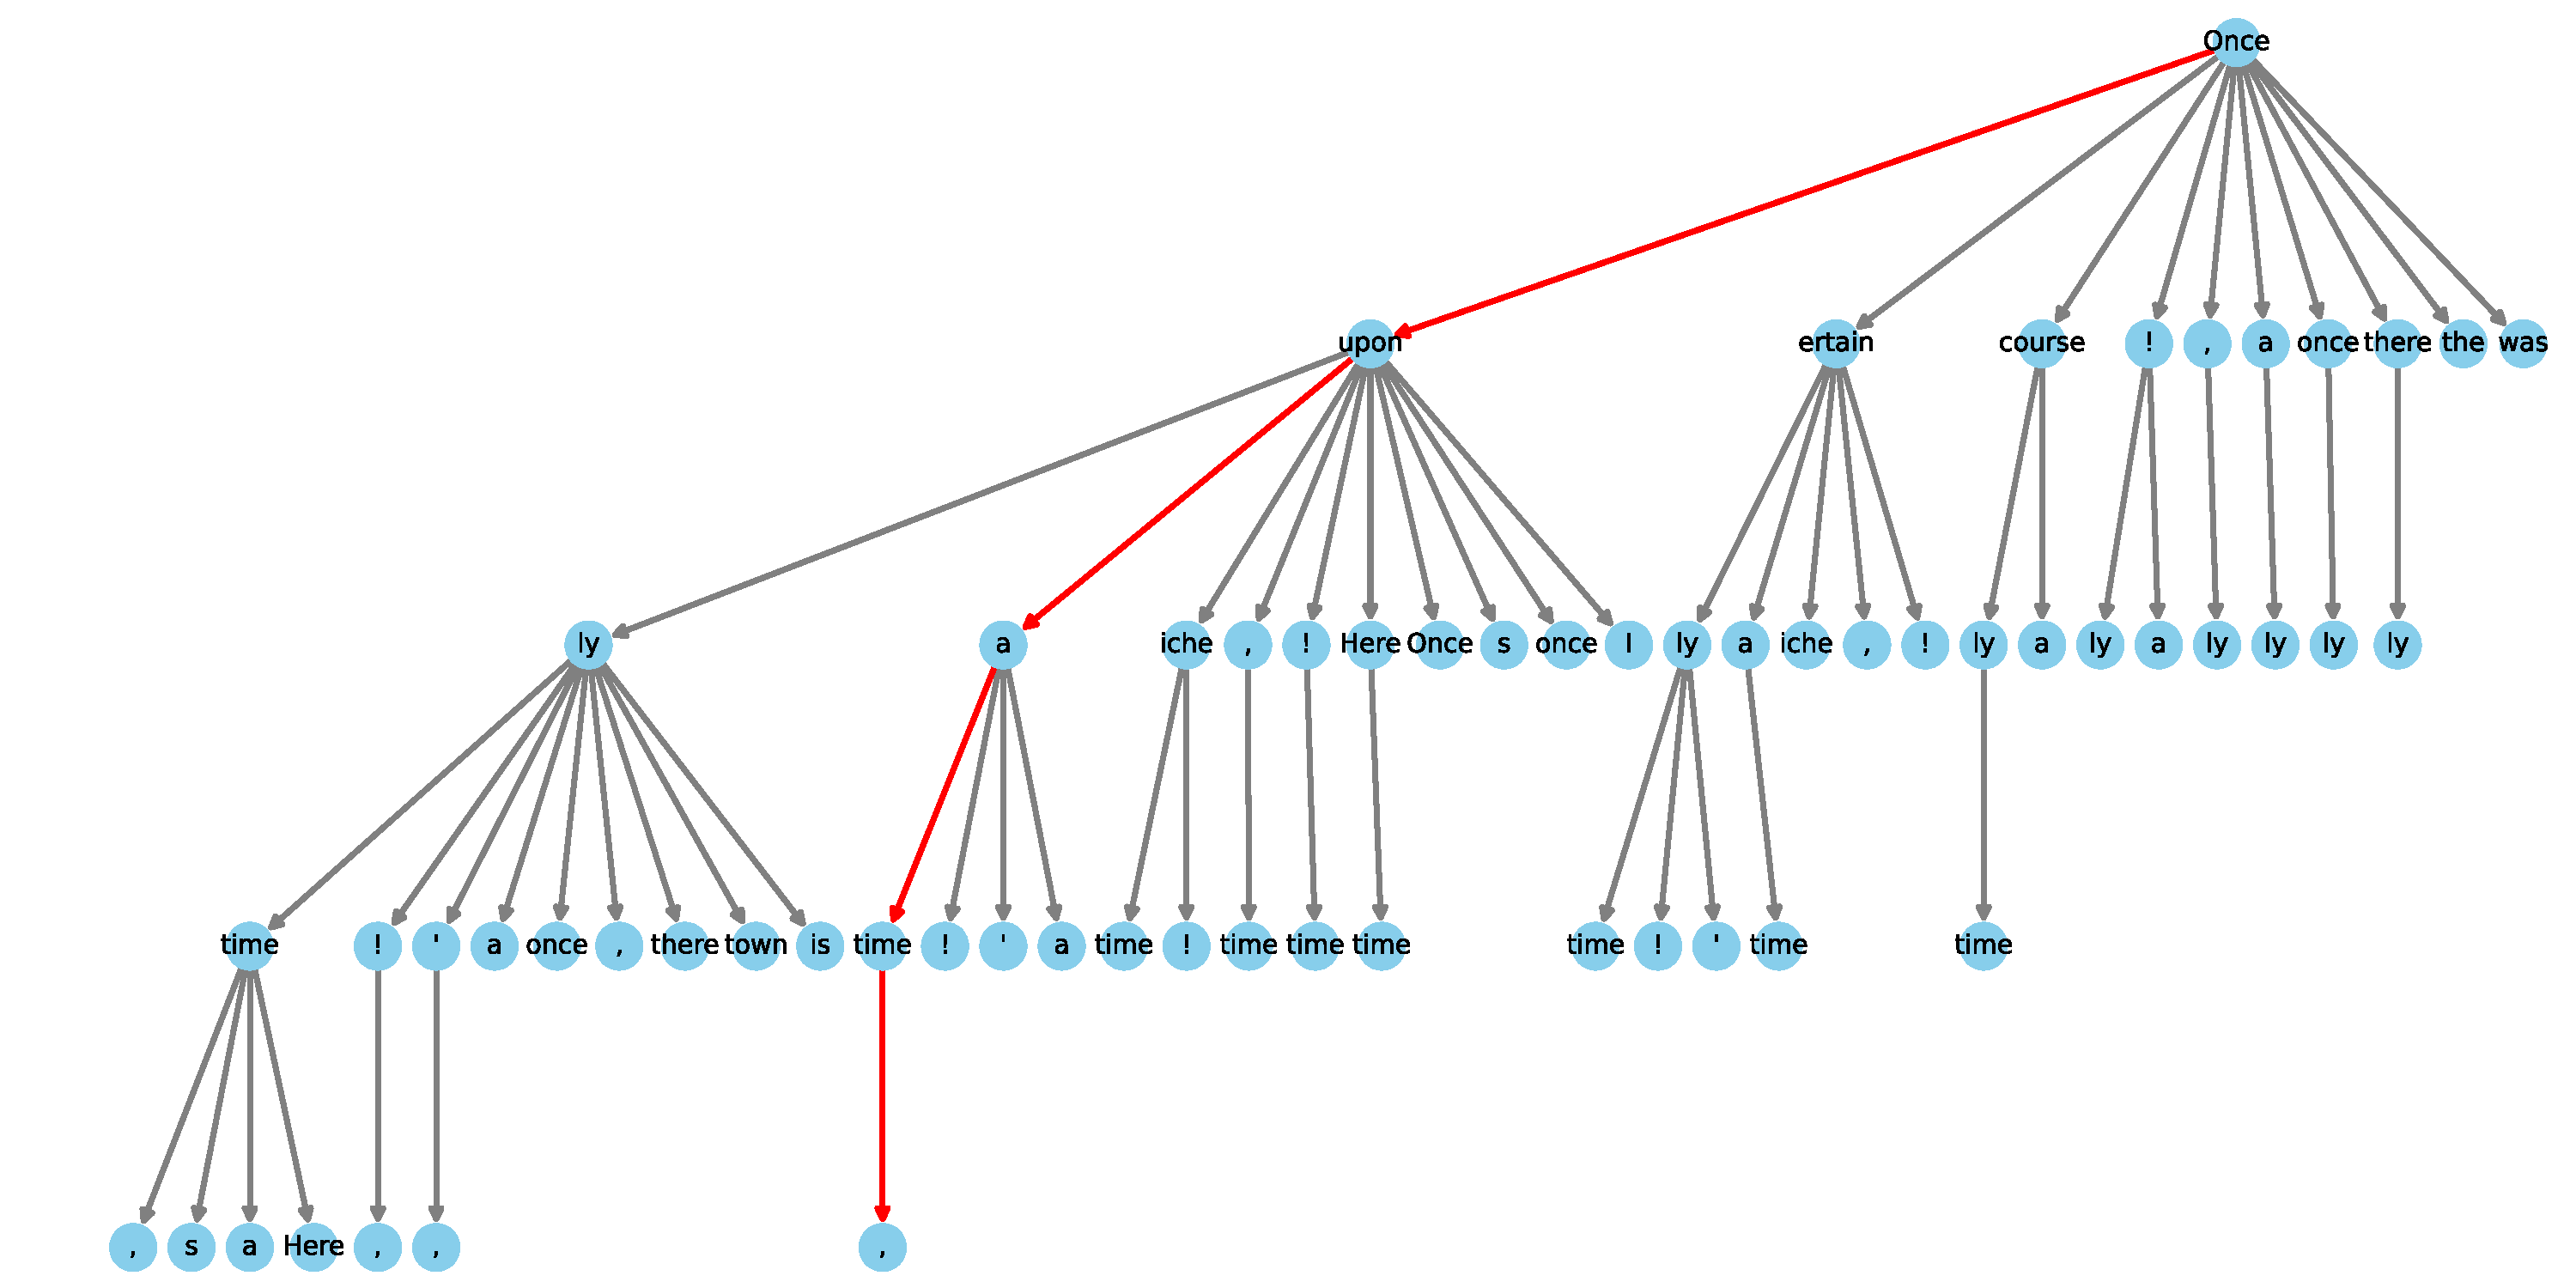
\includegraphics[width=0.6\textwidth]{sparse_tree.pdf}
    \caption{Visualization of a sparse tree setting for \ours-2 Vicuna-7B. The tree has \textcolor{black}{64 nodes representing candidate tokens} and a depth of 4 which indicates 4 \ours heads involved in calculation. Each node indicates a token from a top-k prediction of a \ours head, and the edges show the connections between them. The red lines highlight the path that correctly predicts the future tokens.}
    \label{fig:sparse_tree}
\end{figure*}

\section{Results of Speculative Decoding}\label{appendix:spec}

In this study, speculative decoding was applied to Vicuna models~\citep{vicuna2023} with varying sizes, specifically 7B, 13B, and 33B. The preliminary framework utilized open-source models such as Llama-68M and 160M~\citep{miao2023specinfer}, alongside Tiny-Llama~\citep{zhang2024tinyllama} and Tiny-Vicuna~\citep{tiny_vicuna_1b}, fine-tuned from Tiny-Llama with the Vicuna-style instructional tuning strategy. Due to the proprietary nature of speculative decoding methods~\citep{chen2023accelerating, leviathan2022fast}, open-source alternatives\footnote{\href{https://github.com/feifeibear/LLMSpeculativeSampling}{https://github.com/feifeibear/LLMSpeculativeSampling}} were deployed for evaluation. Additionally, we utilize \verb|torch.compile()| to accelerate the inference speed of draft models.

Our results shown in Fig.~\ref{fig:speculative_decoding}, reveal that the optimal settings of the draft model vary with the Vicuna model sizes. Specifically, the Llama-68M, with a setting of the draft token number $\gamma=4$, yielded the best performance for Vicuna-7B, while the same draft model with $\gamma=3$ was most effective for Vicuna-13B. For the larger Vicuna-33B, the Tiny-Vicuna \textcolor{black}{(Vicuna-1B)}, with $\gamma=3$, provided the greatest acceleration. These results suggest that the choice and setting of the drafting model should be tailored to the size of the LLMs, presenting an area for further exploration in the field.



\begin{figure*}[h]
     \centering
     \begin{subfigure}[b]{0.32\textwidth}
         \centering
         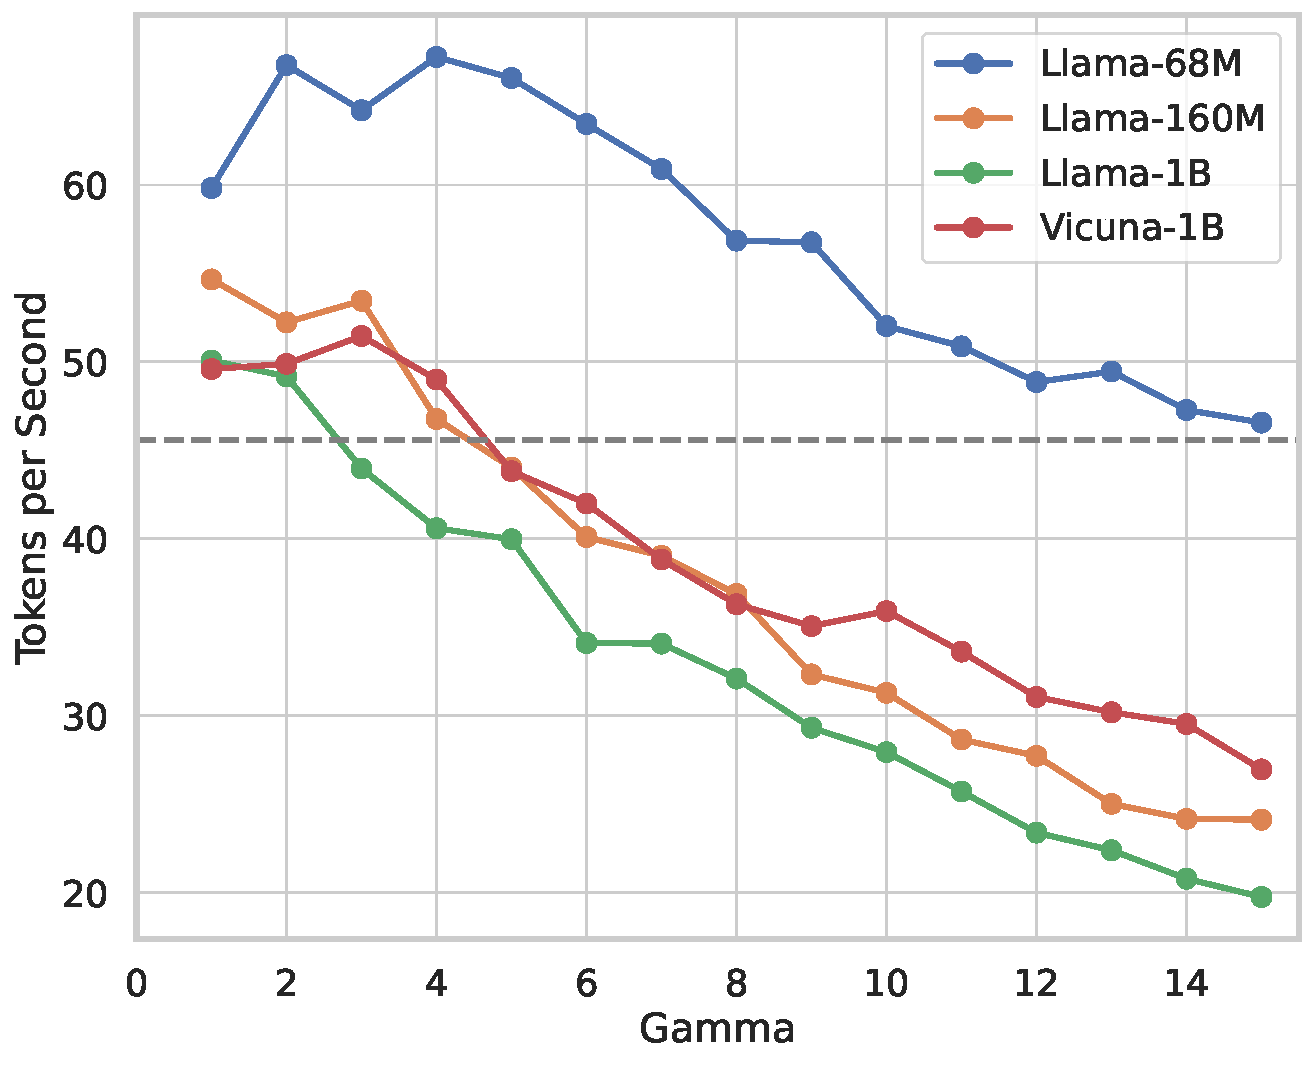
\includegraphics[width=\textwidth]{spec_7b.pdf}
         \caption{Vicuna-7B}
         \label{fig:spec7b}
     \end{subfigure}
     \begin{subfigure}[b]{0.32\textwidth}
         \centering
         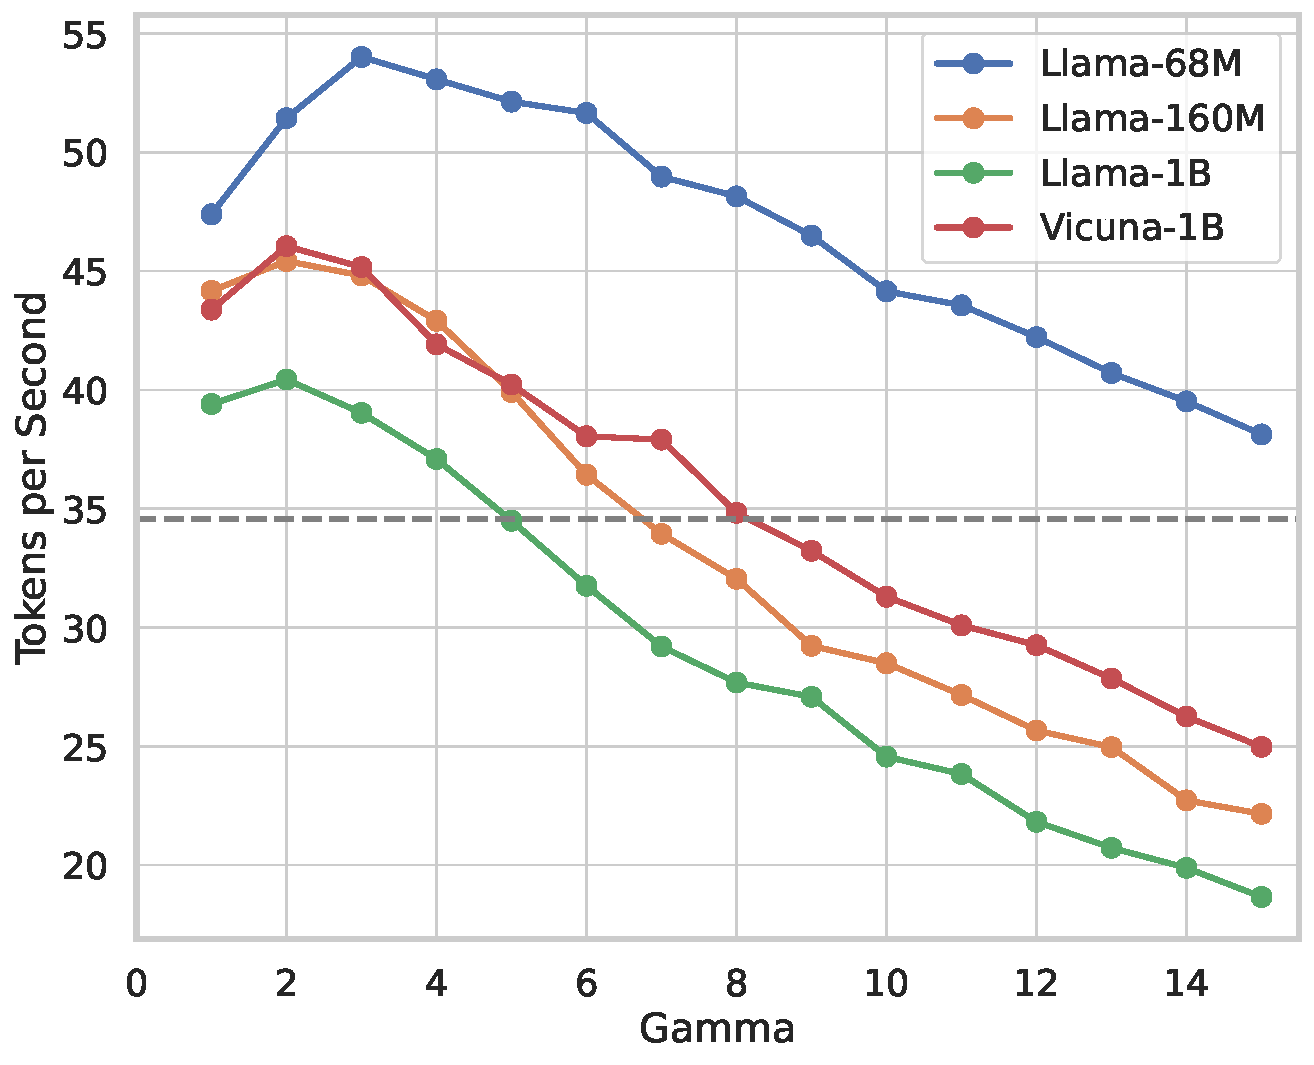
\includegraphics[width=\textwidth]{spec_13b.pdf}
         \caption{Vicuna-13B}
         \label{fig:spec13b}
     \end{subfigure}
    \begin{subfigure}[b]{0.32\textwidth}
         \centering
         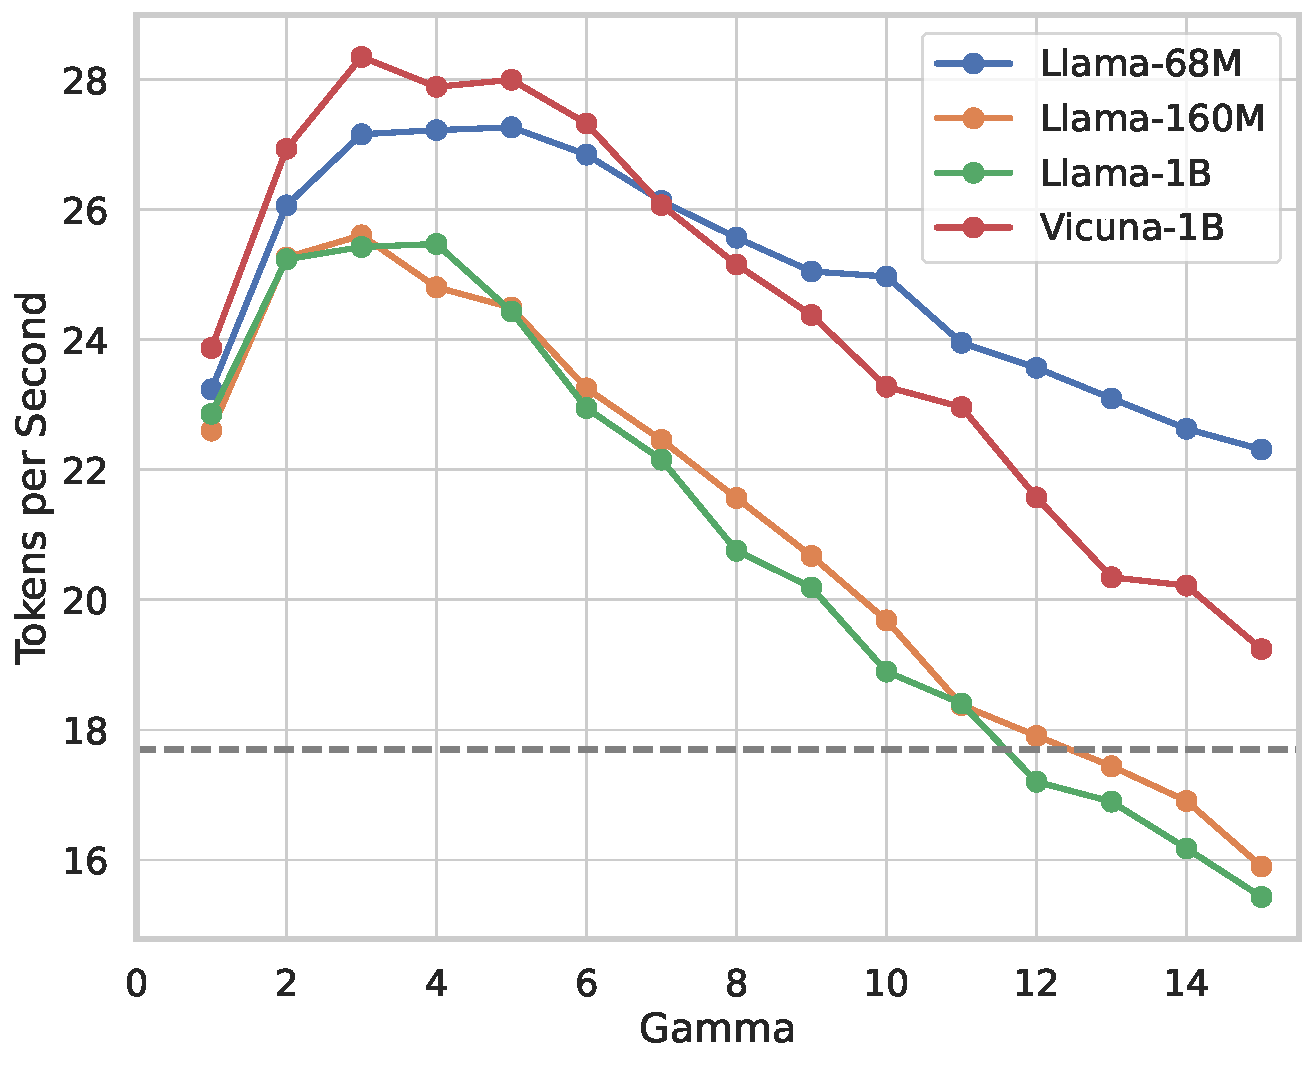
\includegraphics[width=\textwidth]{spec_33b.pdf}
         \caption{Vicuna-33B}
         \label{fig:spec33b}
     \end{subfigure}
        \caption{Inference speed of various models using speculative decoding on MT-Bench. Baseline model speeds are presented by grey dotted lines for comparison. $\gamma$ denotes the draft token number.}
        \label{fig:speculative_decoding}
\end{figure*}

\section{Additional Results for All Models}\label{appendix:add_results}
We show speedup on various models in Fig.~\ref{fig:speedup_model_wild}.
\begin{figure}[h]
    \centering
    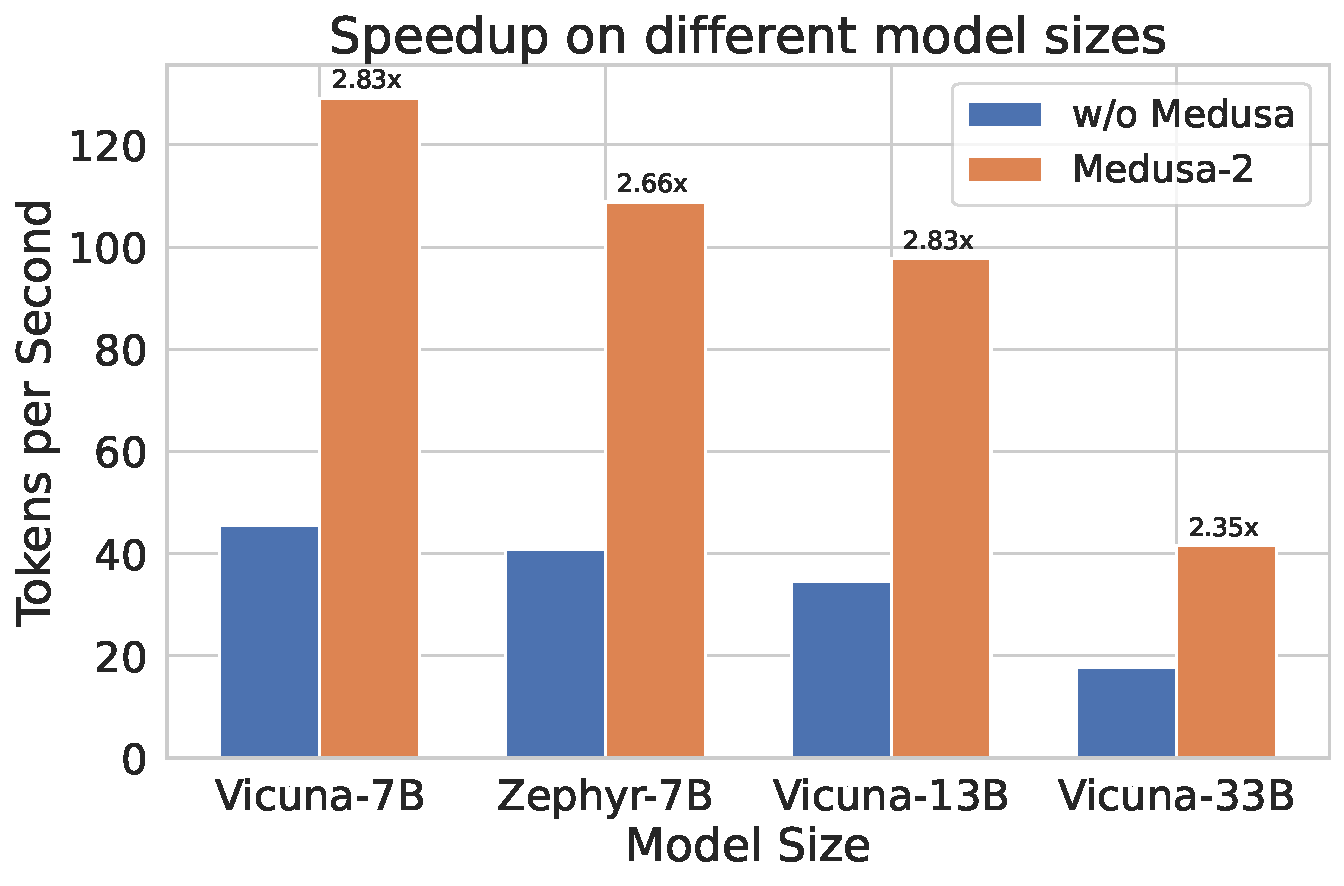
\includegraphics[width=0.45\textwidth]{speedup_model_wild_wide.pdf}
    \caption{Speedup of various models with \ours-2. \ours-2 shows significant speed improvement over all the models, while models trained with self-distillation \textcolor{black}{(Zephyr-7B, Vicuna-13/33B)} have weaker speedup due to the trade-off between preserving quality and boosting speed.}
    \label{fig:speedup_model_wild}
\end{figure}


\section{Additional Results on AlpacalEval Dataset}
We conduct further experiments on the AlpacaEval~\citep{alpaca_eval} dataset. \ours-2 achieves consistent speedup similar to the results on MT-Bench.
\begin{table}[h]
    \centering
    \begin{tabular}{llrrrr}
    \toprule
     & Model & Base speed (tokens/s) & \ours speed (tokens/s) & Acc. rate & Speedup \\
    \midrule
     & Vicuna-7b & 37.07 & 106.76 & 3.23 & 2.88 \\
     & Vicuna-13b & 29.01 & 91.54 & 3.28 & 3.16 \\
     & Vicuna-33b & 17.87 & 40.43 & 2.85 & 2.26 \\
     & Zephyr-7b & 34.21 & 99.50 & 3.08 & 2.91 \\
    \bottomrule
    \end{tabular}
    \caption{Speedup results on AlpacaEval~\citep{alpaca_eval} dataset.}
    \label{tab:alpaca_eval_speedup}
\end{table}

\section{Exploration and Modeling of Hardware Constraints and \ours}~\label{sec:roofline}


We explore the hardware constraints, specifically memory-bandwidth bound, and their impact on \ours-style parallel decoding by incorporating a simplified \textcolor{black}{Llama-series} model.
First, we \textcolor{black}{identify} that the operators involving matrix multiplications, such as linear layers and attention matrix multiplications, are the primary sources of overhead. We profile the performance of FLOP/s vs. Operational Intensity \textcolor{black}{which is the ratio of FLOP/s to bandwidth (bytes/s)}, across various GPUs, including the A100-80GB-PCIe, A40, and A6000.
Next, we examine the changes in FLOP/s vs. Operational Intensity when using \ours for different operators.
Finally, we apply a straightforward analytical model to calculate acceleration rates and combine it with hardware benchmarks. This provides insights into the effects under different model sizes, sequence lengths, and batch sizes.

\subsection{Roofline Model of Operators}
We present an analysis of the roofline model for various operators in large language models (LLMs), specifically focusing on Llama-7B, Llama-13B, and Llama-33B~\cite{touvron2023llama}. These models were benchmarked on different GPUs, including the A100-80GB-PCIe, A40, and A6000. We looked into the three categories of matrix multiplication operators since they represent the primary sources of computational overhead in these models. Our study follows the report~\cite{chen2023transformer} which investigates the effectiveness of batch size but ours focuses more on decoding and parallel decoding.

Table~\ref{tab:complexity} details the computation and space complexity for each operator during the prefill, decoding, and \ours decoding phases. The operators include the linear layers for query, key, and value matrices ($XW_{Q}$, $XW_{K}$, $XW_{V}$), the attention matrix multiplications ($QK^T$, $PV$), and the up/gate/down linear layers ($XW_{u}$, $XW_{g}$, $XW_{d}$).
$b$ stands for the batch size, $s$ stands for the sequence length, $h$ stands for the hidden dimension, $i$ stands for the intermediate dimension, $n$ stands for the number of attention heads, $d$ stands for the head dimension and $q$ stands for the candidate length for \ours.
For more details of these operators please refer to the articles~\cite{touvron2023llama, chen2023transformer}.


\begin{table}[h]
\centering
\caption{Computational and space complexity of the main operators in different phases. \textcolor{black}{The table is based on Table 2 in the report~\cite{chen2023transformer}.}}

\scriptsize
\begin{tabular}{lcccc}
\toprule
 \textbf{Operator} & \textbf{Input Shape} & \textbf{Output Shape} & \textbf{Comp. Complexity} & \textbf{Space Complexity} \\ \midrule
 \textbf{Prefill} \\ \midrule
 $XW_{Q}$, $XW_{K}$, $XW_{V}$ & $(b, s, h)$ & $(b, s, h)$ & $O(bsh^2)$ & $O(2bsh + h^2)$ \\ \midrule
  $QK^T$ & $(b, n, s, d),(b, n, s, d)$ & $(b, n, s, s)$ & $O(bs^2nd)$ & $O(2bsnd + bs^2n)$ \\ 
  $PV$ &$(b, n, s, s),(b, n, s, d)$&$(b, n, s, d)$&& \\ \midrule
  $XW_{u}$, $XW_{g}$ & $(b, s, h)$ & $(b, s, i)$ & $O(bshi)$ & $O(bs(h + i) + hi)$ \\ 
  $XW_{d}$&$(b, s, i)$&$(b, s, h)$&&\\ \midrule
   \textbf{Decoding} \\ \midrule
$XW_{Q}$, $XW_{K}$, $XW_{V}$ & $(b, 1, h)$ & $(b, 1, h)$ & $O(bh^2)$ & $O(2bh + h^2)$ \\ \midrule
  $QK^T$ & $(b, n, 1, d), (b, n, s, d)$ & $(b, n, s, 1)$ & $O(bsnd)$ & $O(bsn + bsnd + bnd)$ \\ 
  $PV$ & $(b, n, s, 1), (b, n, 1, d)$ & $(b, n, 1, d)$ & &  \\ \midrule
  $XW_{u}$, $XW_{g}$ & $(b, 1, h)$ & $(b, 1, i)$ & $O(bhi)$ & $O(b(h + i) + hi)$ \\
  $XW_{d}$ & $(b, 1, i)$ & $(b, 1, h)$ &  & \\\midrule
   \textbf{Parallel decoding} \\ \midrule
 $XW_{Q}$, $XW_{K}$, $XW_{V}$ & $(b, q, h)$ & $(b, q, h)$ & $O(bqh^2)$ & $O(2bqh + h^2)$ \\ \midrule
  $QK^T$ & $(b, n, q, d), (b, n, s, d)$ & $(b, n, s, q)$ & $O(bsqnd)$ & $O(bsqn + b(s+q)nd)$ \\ 
    $PV$ & $(b, n, s, q), (b, n, q, d)$ & $(b, n, q, d)$ & &  \\ \midrule
  $XW_{u}$, $XW_{g}$ & $(b, q, h)$ & $(b, q, i)$ & $O(bqhi)$ & $O(bq(h + i) + hi)$ \\
  $XW_{d}$ & $(b, q, i)$ & $(b, q, h)$ &  \\ \bottomrule
\end{tabular}
\label{tab:complexity}
\end{table}

Figures~\ref{fig:llama7b-roofline-a100}-\ref{fig:llama33b-roofline-a6000} show the benchmark of three categories of operators on different models (7/13/33B) under various settings. To evaluate each operator's performance and throughput, we chose the combination of settings including batch sizes from 1 to 64 in powers of 2 and sequence lengths from 128 to 8192 in powers of 2 \textcolor{black}{(49 settings for each operator)}. 
From all the figures, we observe that the datapoints of each operator in the prefill and decoding stages cluster at very similar positions across all GPUs and for various model sizes. 



During the prefill phase, increasing the batch size changes the FLOP/s of the attention matrix multiplications (see \texttt{`qk/pv init`}) but does not affect the Operational Intensity (refer to the vertical dashed arrow in Fig. 9). 
In contrast, increasing the sequence length impacts both FLOP/s and Operational Intensity in the prefill phase (refer to the diagonal dashed arrow in Fig. 9).
During the decoding phase, the attention matrix multiplications are significantly limited by memory bandwidth. Despite an increase in FLOP/s with changes in batch size and sequence length, the Operational Intensity remains nearly unchanged (see \texttt{`qk/pv ar`}). This indicates suboptimal resource utilization in the self-attention mechanism.

The linear layers in the prefill phase are mostly compute-bound (see \texttt{`qkv mlp init`} and \texttt{`up/gate/down init`}). During the decoding phase, the datapoints of the linear layer form a line with the same slope as the GPU’s memory bandwidth (see \texttt{`qkv mlp ar`} and \texttt{`up/gate/down ar`}). This indicates the linear layers in the decoding stage are also bounded by memory bandwidth. Increasing the batch size improves the achieved FLOP/s and Operational Intensity under memory bandwidth constraints through better parallelism. Note that linear layers only process the new token and are independent of sequence length (See `Decoding` section in Table~\ref{tab:complexity}).

\begin{figure}[h]
    \centering
    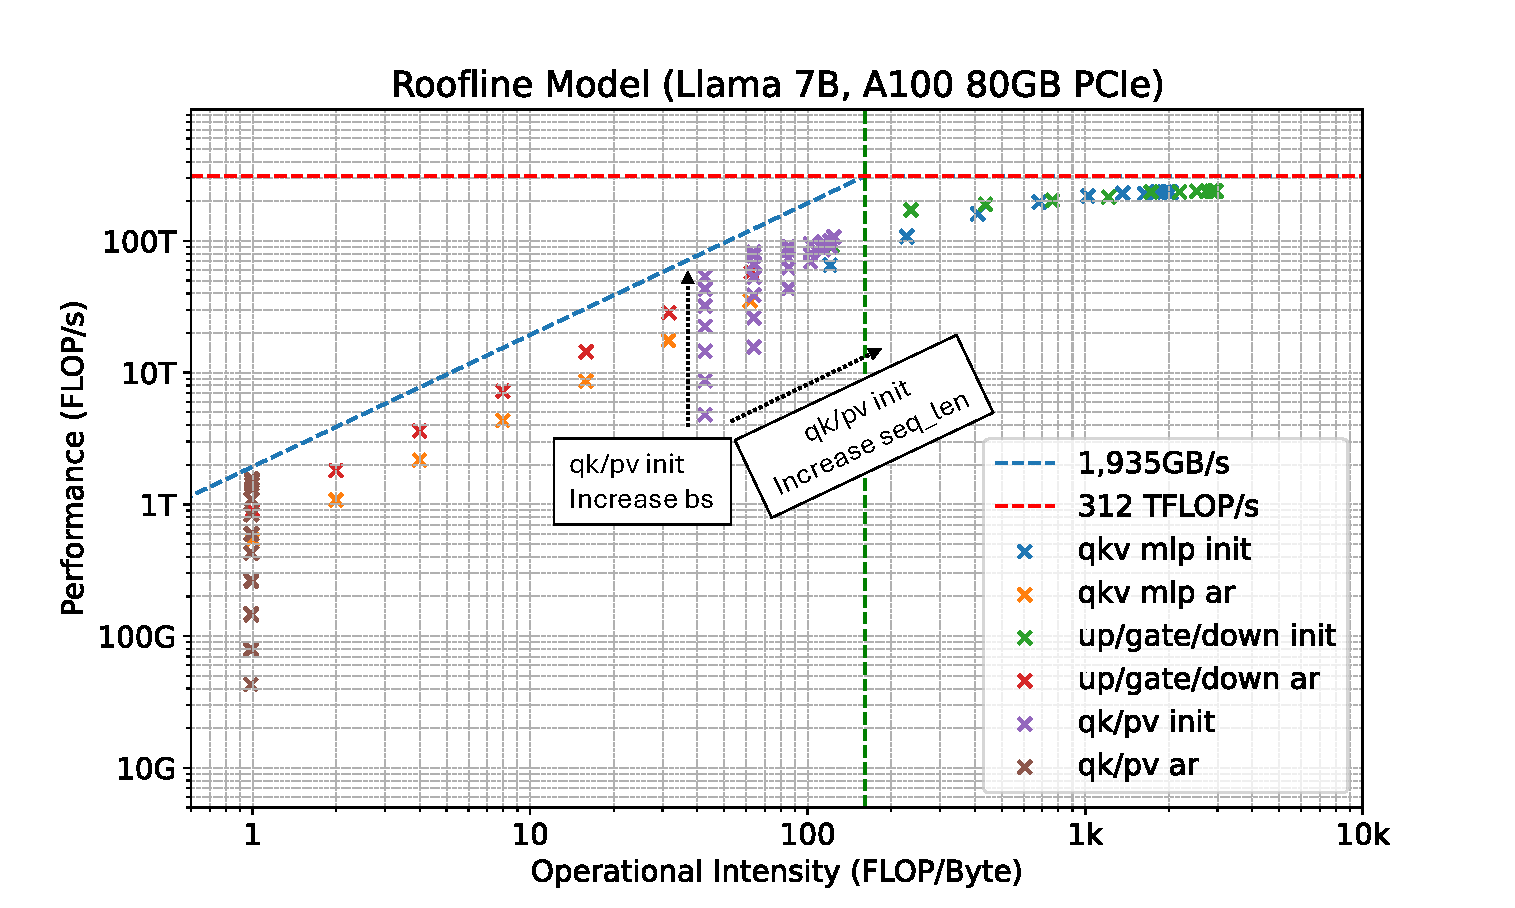
\includegraphics[width=0.8\textwidth]{llama7b-roofline-a100.pdf}
    \caption{The figure shows the relationship between FLOP/s and Operational Intensity for all benchmarked datapoints of Llama-7B operators on A100-80GB-PCIe. The dashed lines represent the HBM bandwidth limit (1,935GB/s) and the peak performance limit (312 TFLOP/s)~\cite{nvidia_a100_datasheet}. `\texttt{qkv mlp}' stands for the linear layers projecting hidden features to query/key/value features. `\texttt{up/gate/down}' stands for the linear layers following the attention block. `\texttt{qk/pv}' stands for the two steps of attention matrix multiplications. `\texttt{ar}' stands for the decoding (autoregressive) and `\texttt{init}' stands for the prefill phase.}
    \label{fig:llama7b-roofline-a100}
\end{figure}

\begin{figure}[h]
    \centering
    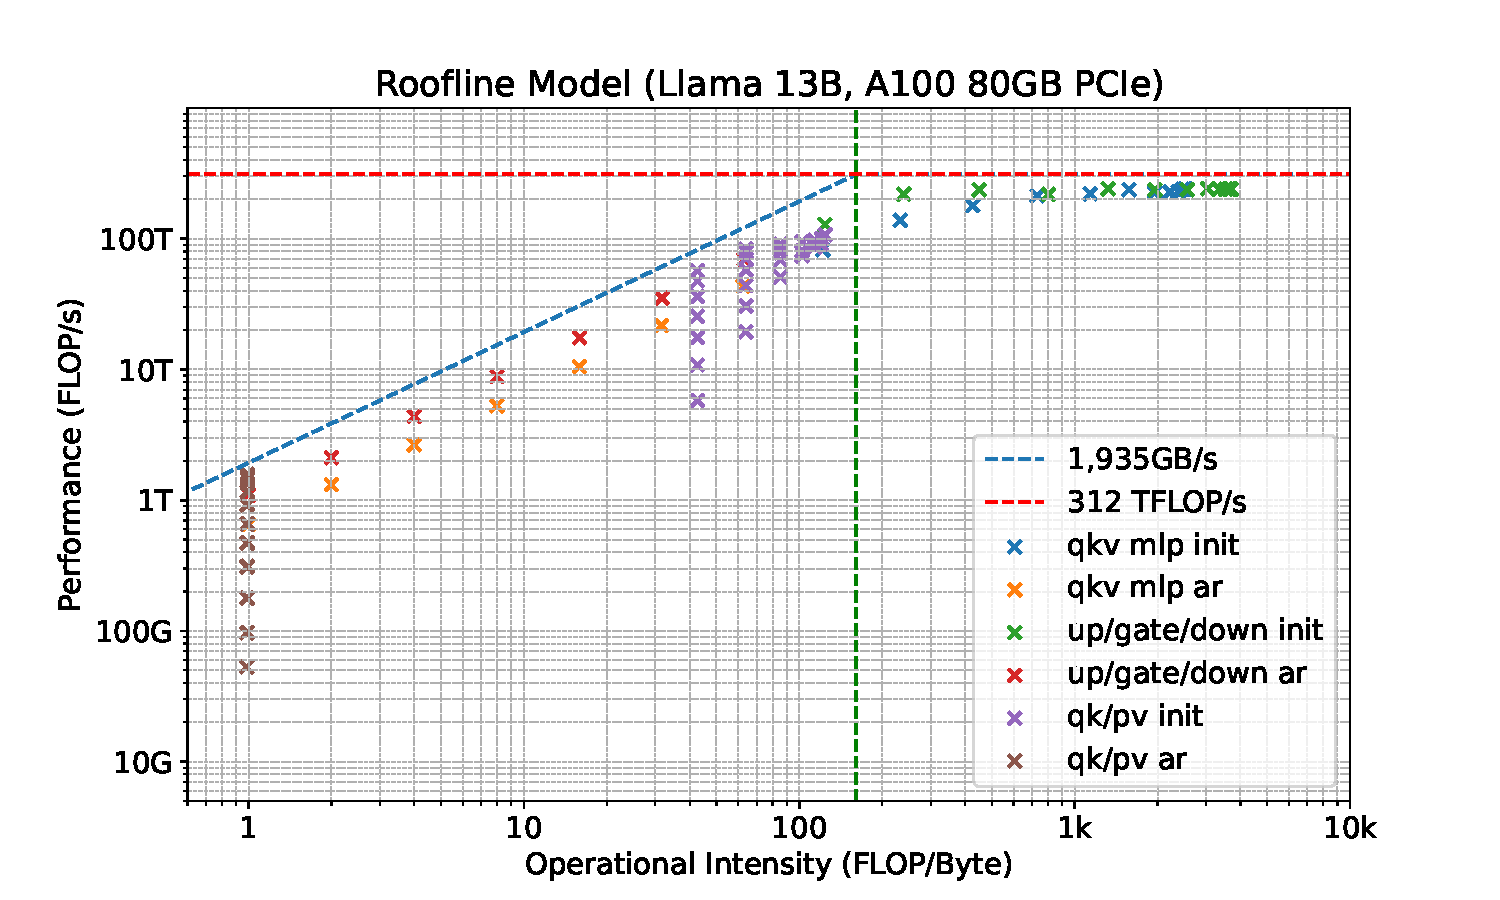
\includegraphics[width=0.8\textwidth]{llama13b-roofline-a100.pdf}
    \caption{Llama-13B operators on A100-80GB-PCIe.}
    \label{fig:llama13b-roofline-a100}
\end{figure}

\begin{figure}[h]
    \centering
    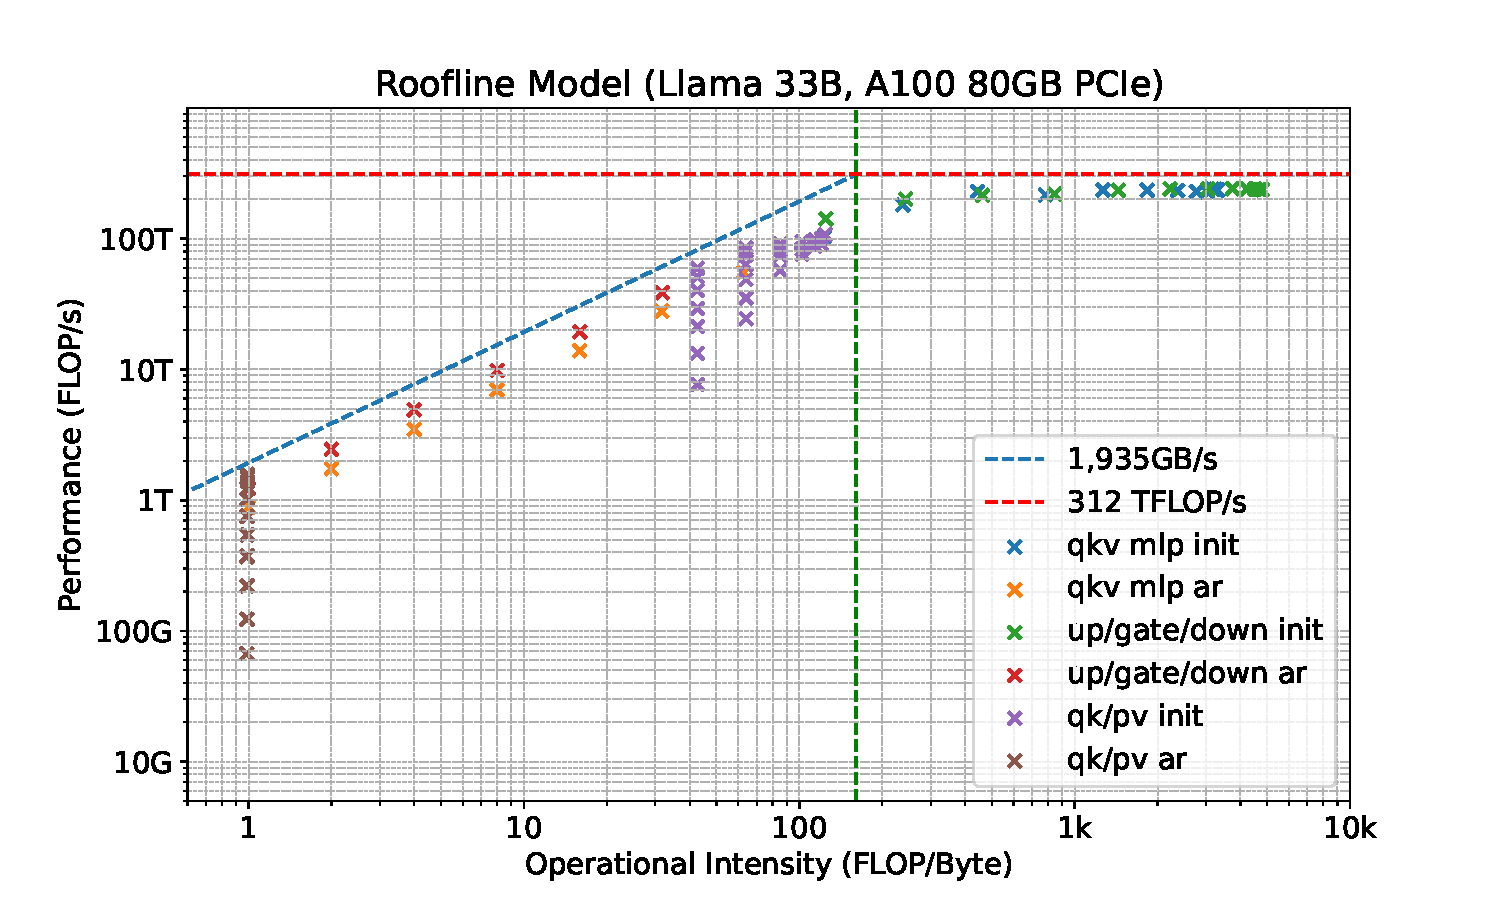
\includegraphics[width=0.8\textwidth]{llama33b-roofline-a100.pdf}
    \caption{Llama-33B operators on A100-80GB-PCIe.}
    \label{fig:llama33b-roofline-a100}
\end{figure}

\begin{figure}[h]
    \centering
    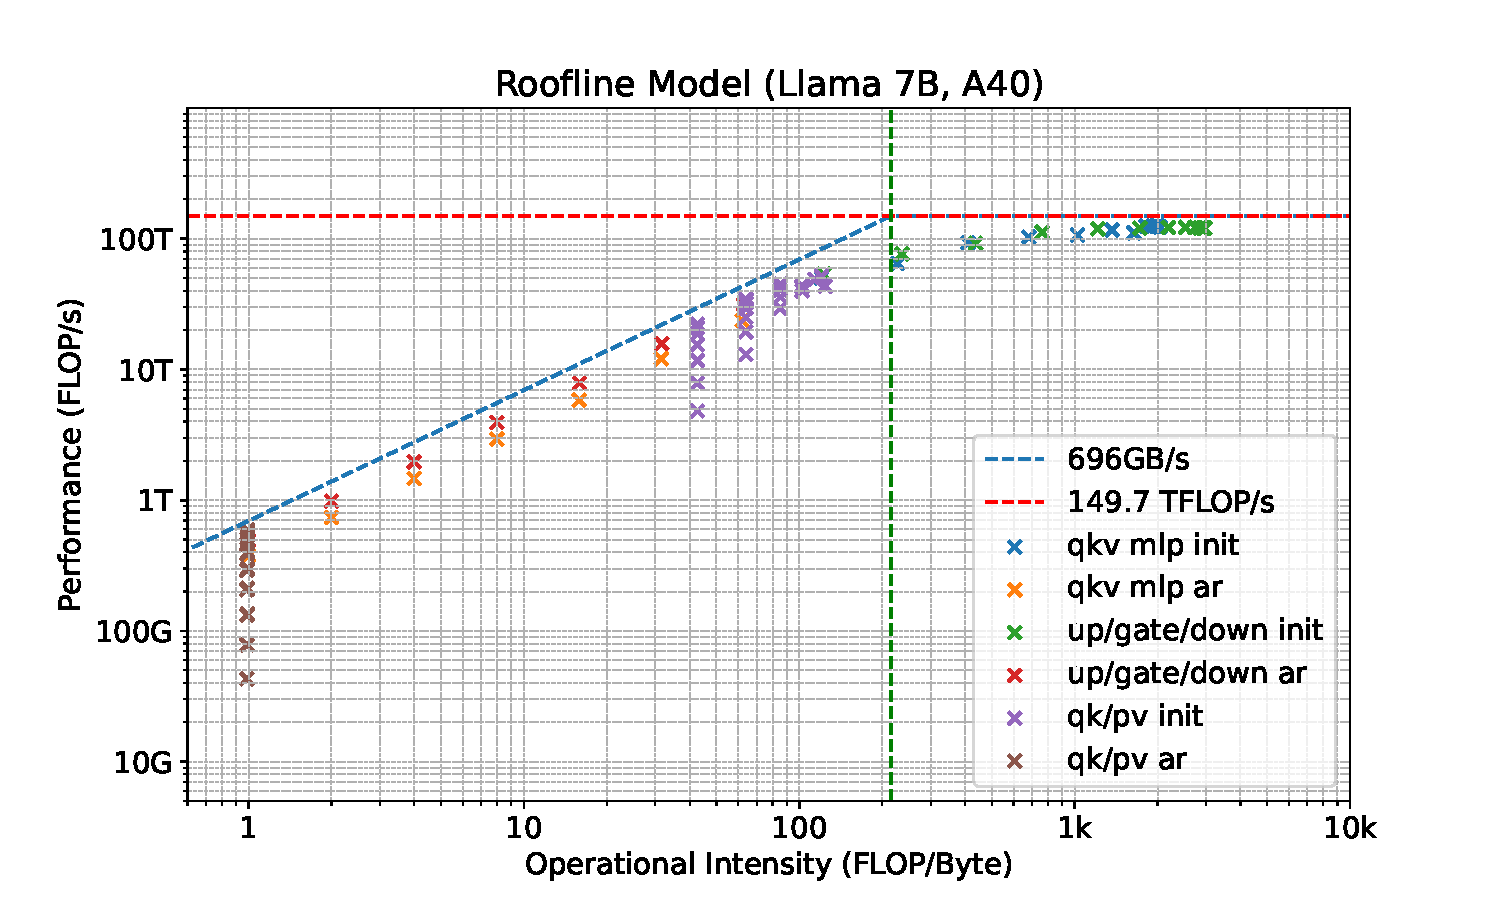
\includegraphics[width=0.8\textwidth]{llama7b-roofline-a40.pdf}
    \caption{Llama-7B operators on A40.}
    \label{fig:llama7b-roofline-a40}
\end{figure}


\begin{figure}[h]
    \centering
    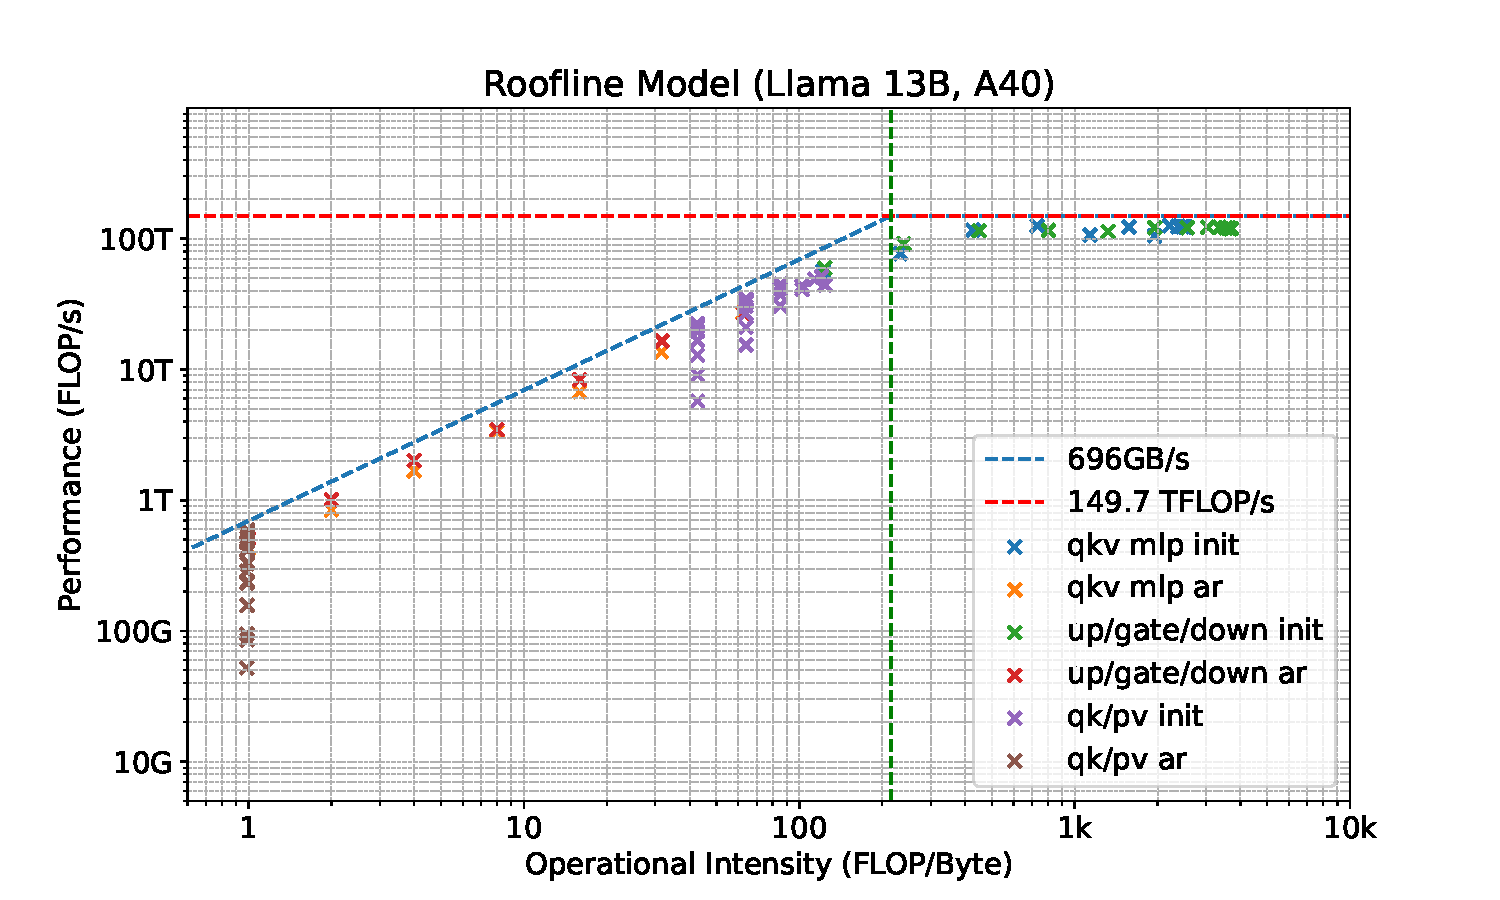
\includegraphics[width=0.8\textwidth]{llama13b-roofline-a40.pdf}
    \caption{Llama-13B operators on A40.}
    \label{fig:llama13b-roofline-a40}
\end{figure}


\begin{figure}[h]
    \centering
    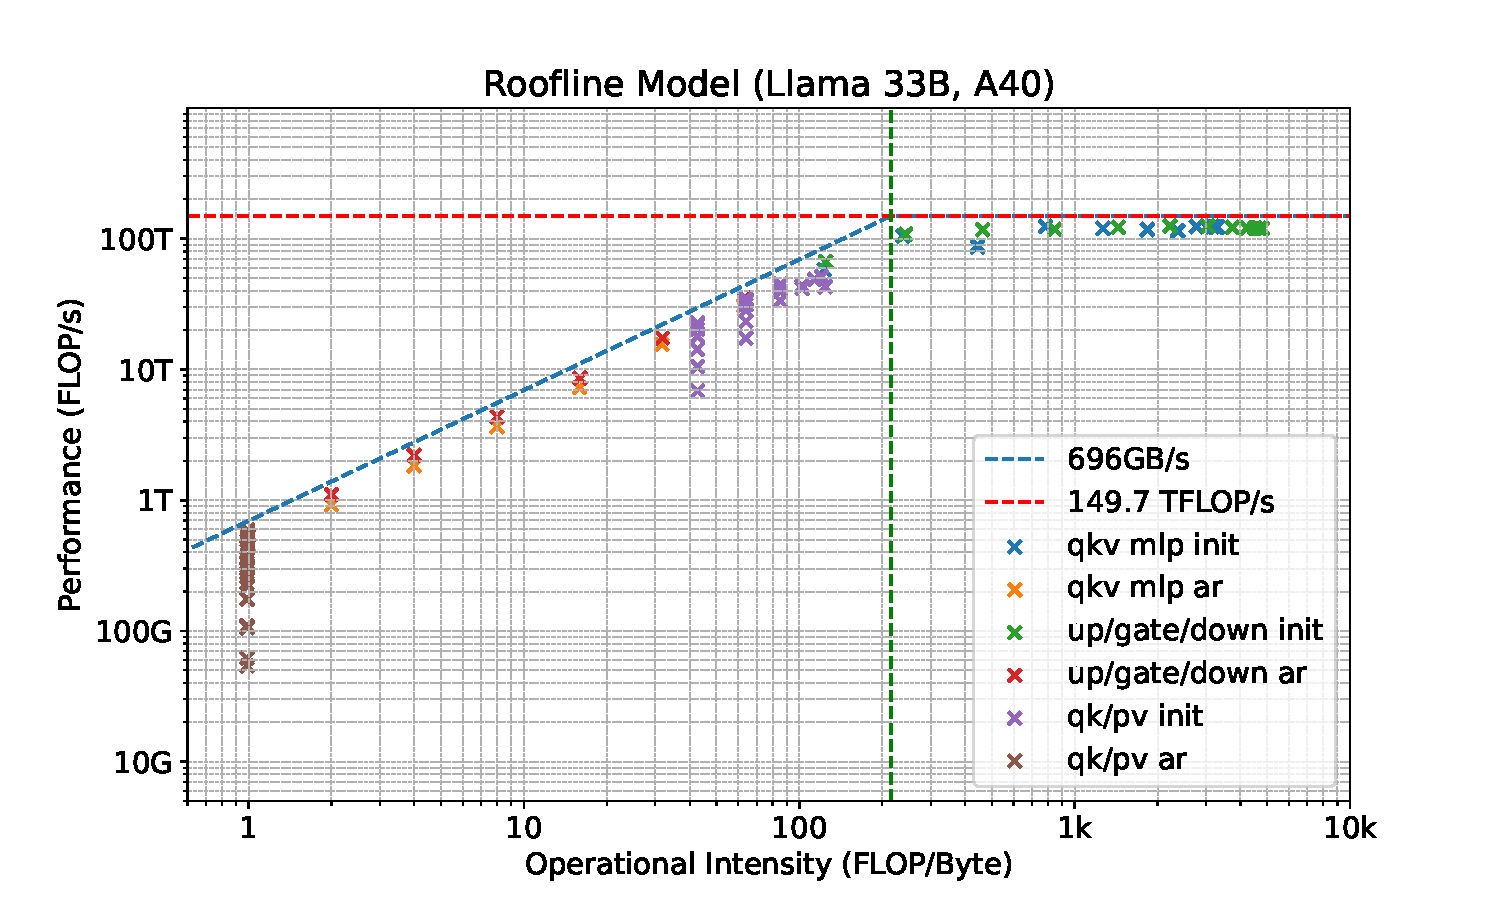
\includegraphics[width=0.8\textwidth]{llama33b-roofline-a40.pdf}
    \caption{Llama-33B operators on A40.}
    \label{fig:llama33b-roofline-a40}
\end{figure}



\begin{figure}[h]
    \centering
    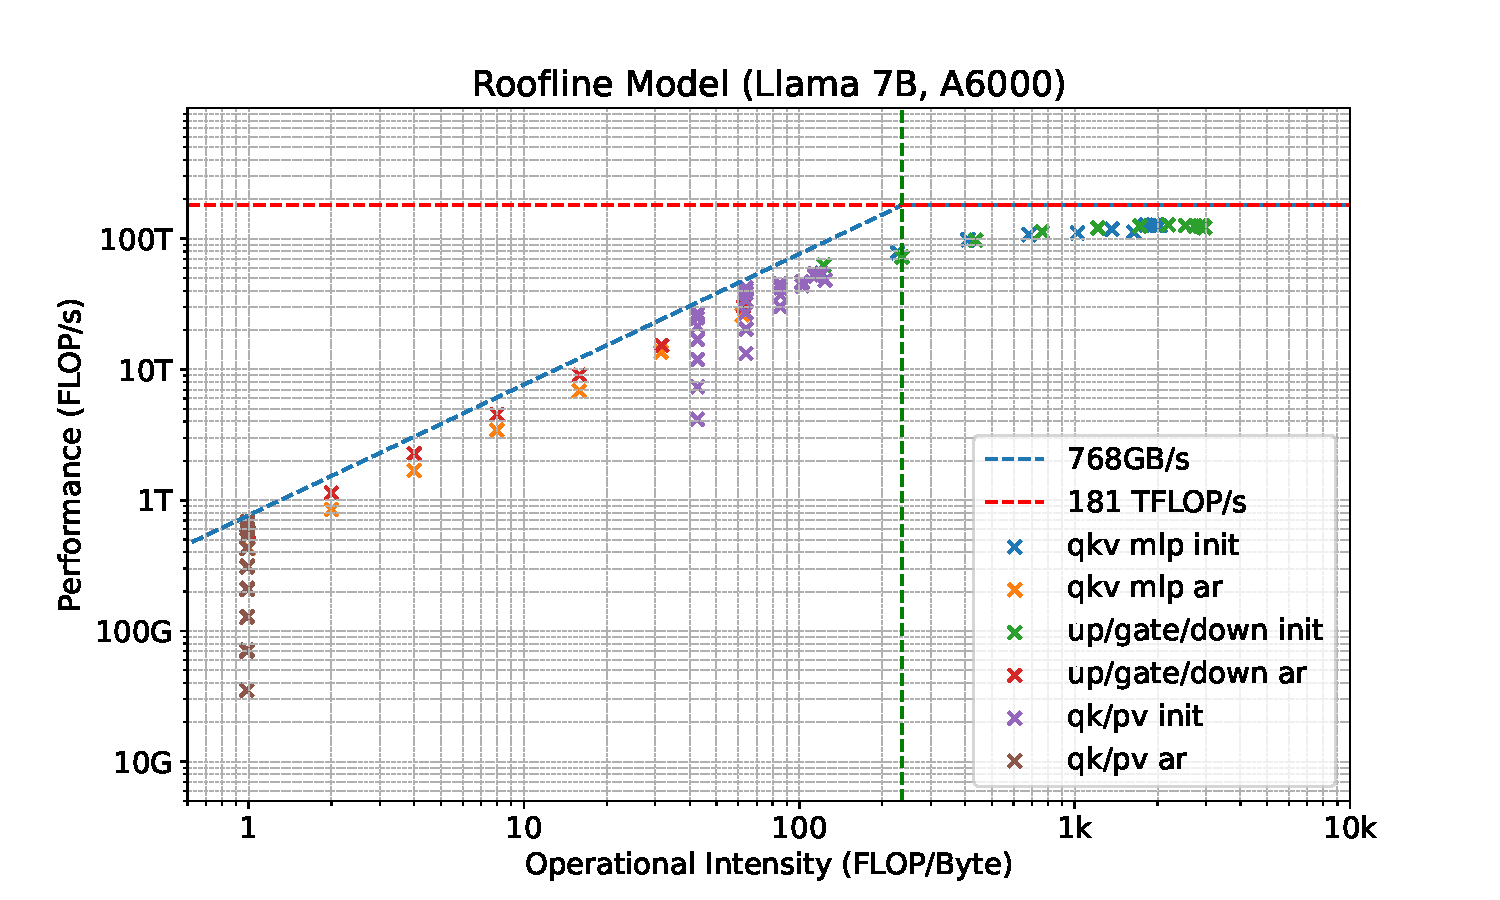
\includegraphics[width=0.8\textwidth]{llama7b-roofline-a6000.pdf}
    \caption{Llama-7B operators on A6000.}
    \label{fig:llama7b-roofline-a6000}
\end{figure}

\begin{figure}[h]
    \centering
    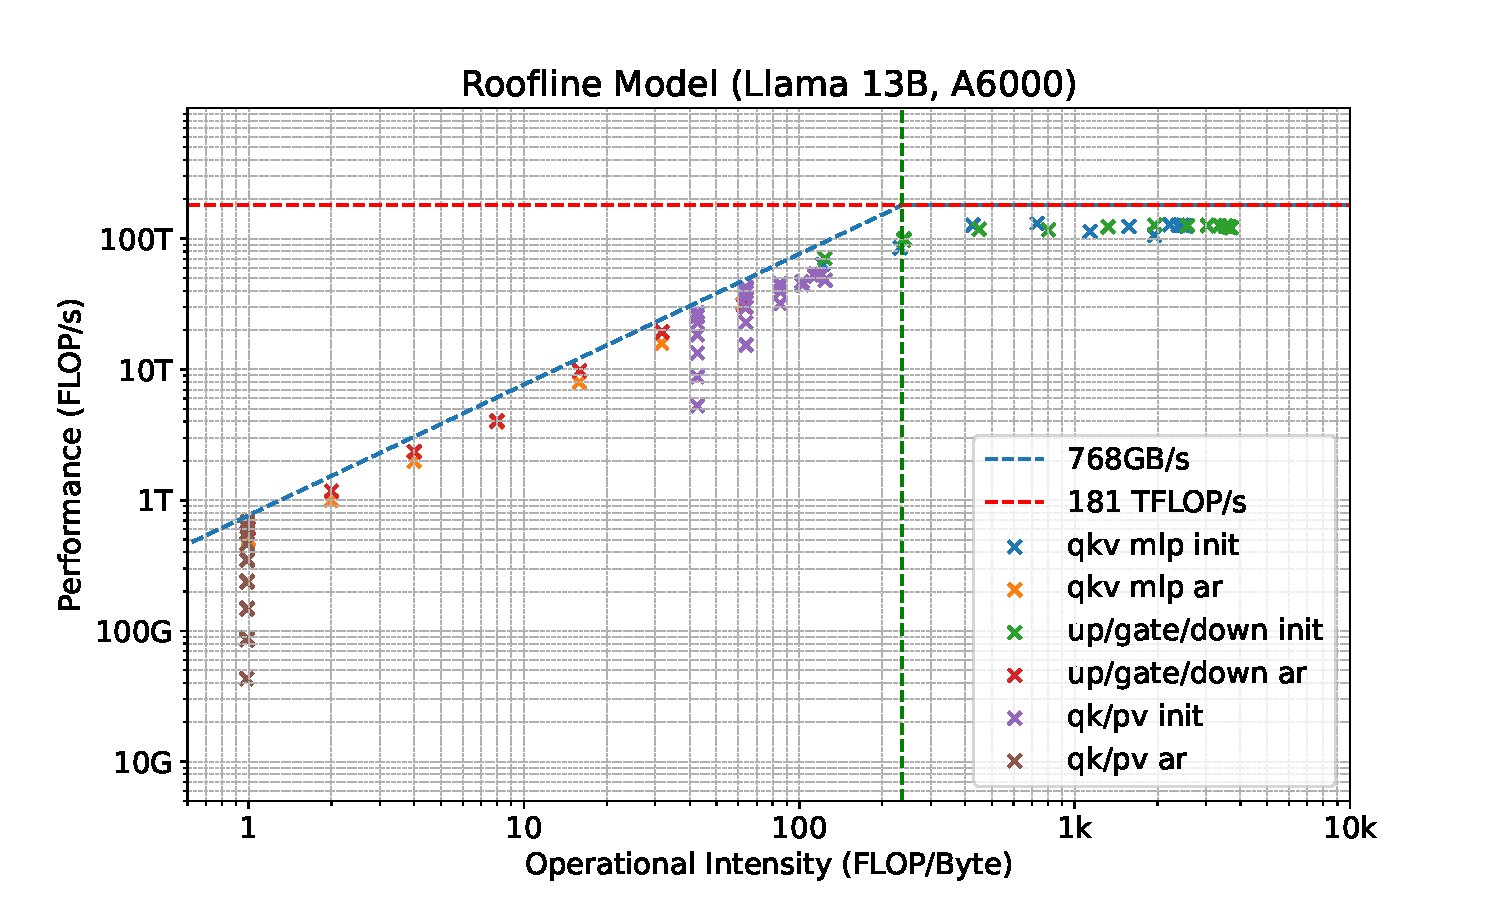
\includegraphics[width=0.8\textwidth]{llama13b-roofline-a6000.pdf}
    \caption{Llama-13B operators on A6000.}
    \label{fig:llama13b-roofline-a6000}
\end{figure}

\begin{figure}[h]
    \centering
    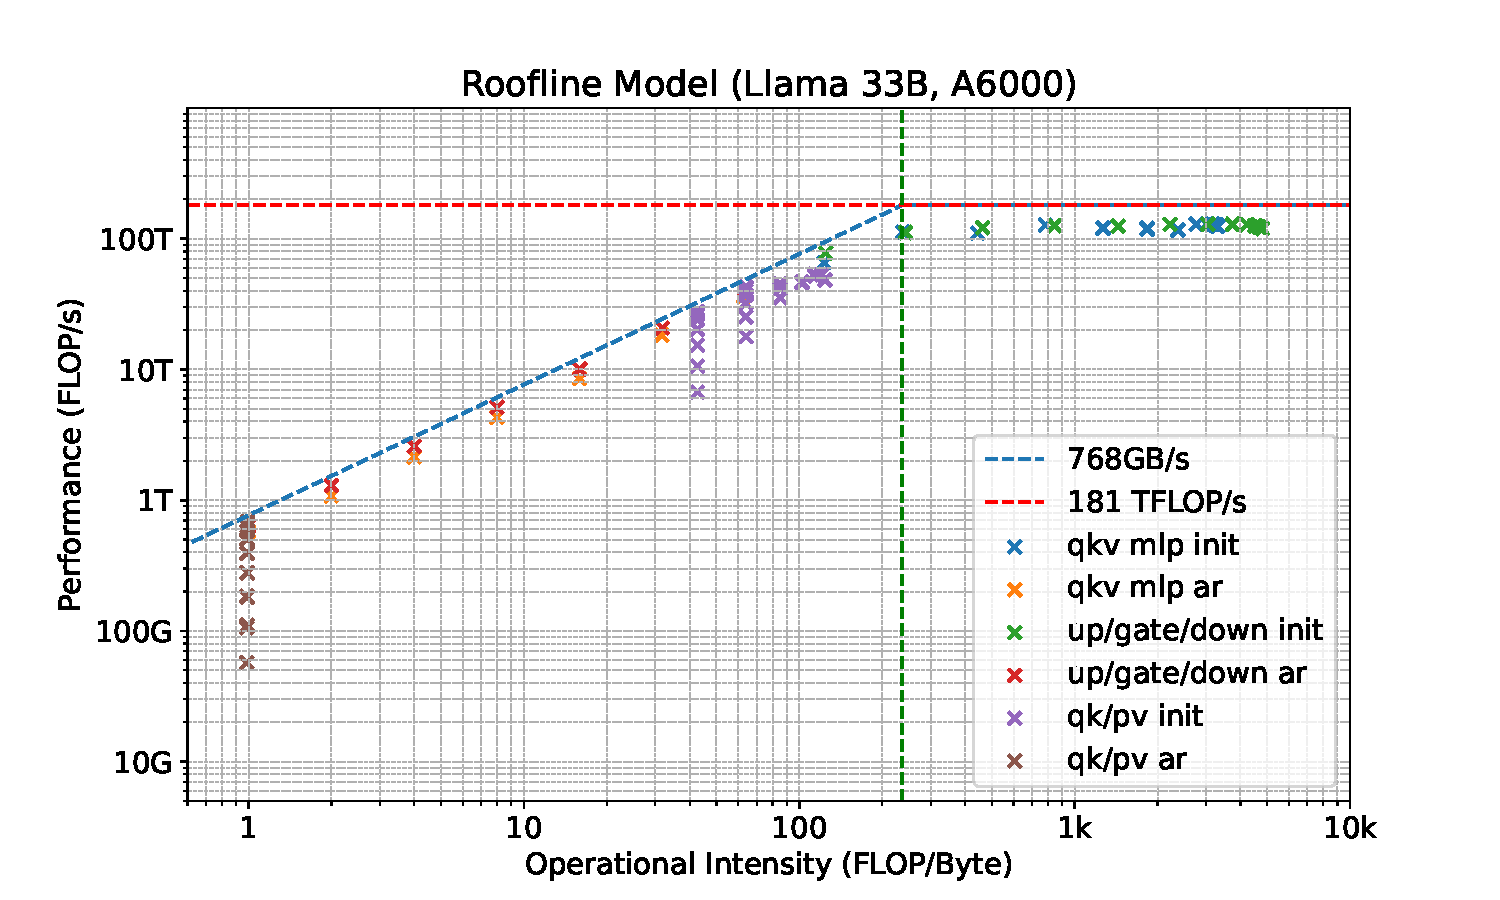
\includegraphics[width=0.8\textwidth]{llama33b-roofline-a6000.pdf}
    \caption{Llama-33B operators on A6000.}
    \label{fig:llama33b-roofline-a6000}
\end{figure}

\clearpage



\subsection{FLOP/s vs. Operational Intensity Variations in \ours}

We investigate how Medusa can change Operational Intensity and elevate the FLOP/s.
We choose Llama 33B on A100-80GB-PCIe as the setting. 

First, we examine the attention matrix multiplication. Fig.~\ref{fig:llama33b-spec-bs16} and Table~\ref{tab:llama33b-spec-bs16} illustrate the effects of \ours while keeping the batch size fixed at 16. We observe increased FLOP/s and Operational Intensity as more candidate tokens are added (original decoding results are plotted as grey dots). This indicates that \ours can leverage additional candidate tokens to improve computational throughput. Compared to regular decoding, \ours achieves 44$\times$ FLOP/s and 41$\times$ Operational Intensity under the setting of batch size 16 and sequence length 1024 with 64 candidate tokens.
 Fig.~\ref{fig:llama33b-spec-seq1024} and Table~\ref{tab:llama33b-spec-seq1024} illustrate the effects of \ours decoding while keeping the sequence length fixed at 1024. Increasing the batch size does not improve Operational Intensity in this scenario. 

Next, we examine the linear layer, focusing on the up/gate/down linear layers. The results are shown in Fig.~\ref{fig:llama33b-spec--mlp-bsall} and Table~\ref{tab:llama33b-spec--mlp-bsall}. \textcolor{black}{Since the linear layers in the decoding phase only process the future tokens while the past tokens are cached, they are independent of the sequence length.} We vary the batch size to observe the effects. As \ours increases the number of candidate tokens with the increasing batch size, we observe a shift from a memory-bandwidth-bound region to a computation-bound region. This shift demonstrates how \ours can transition the performance characteristics of the linear layers from being limited by memory bandwidth to being limited by computational capacity.

\begin{figure}[h]
    \centering
    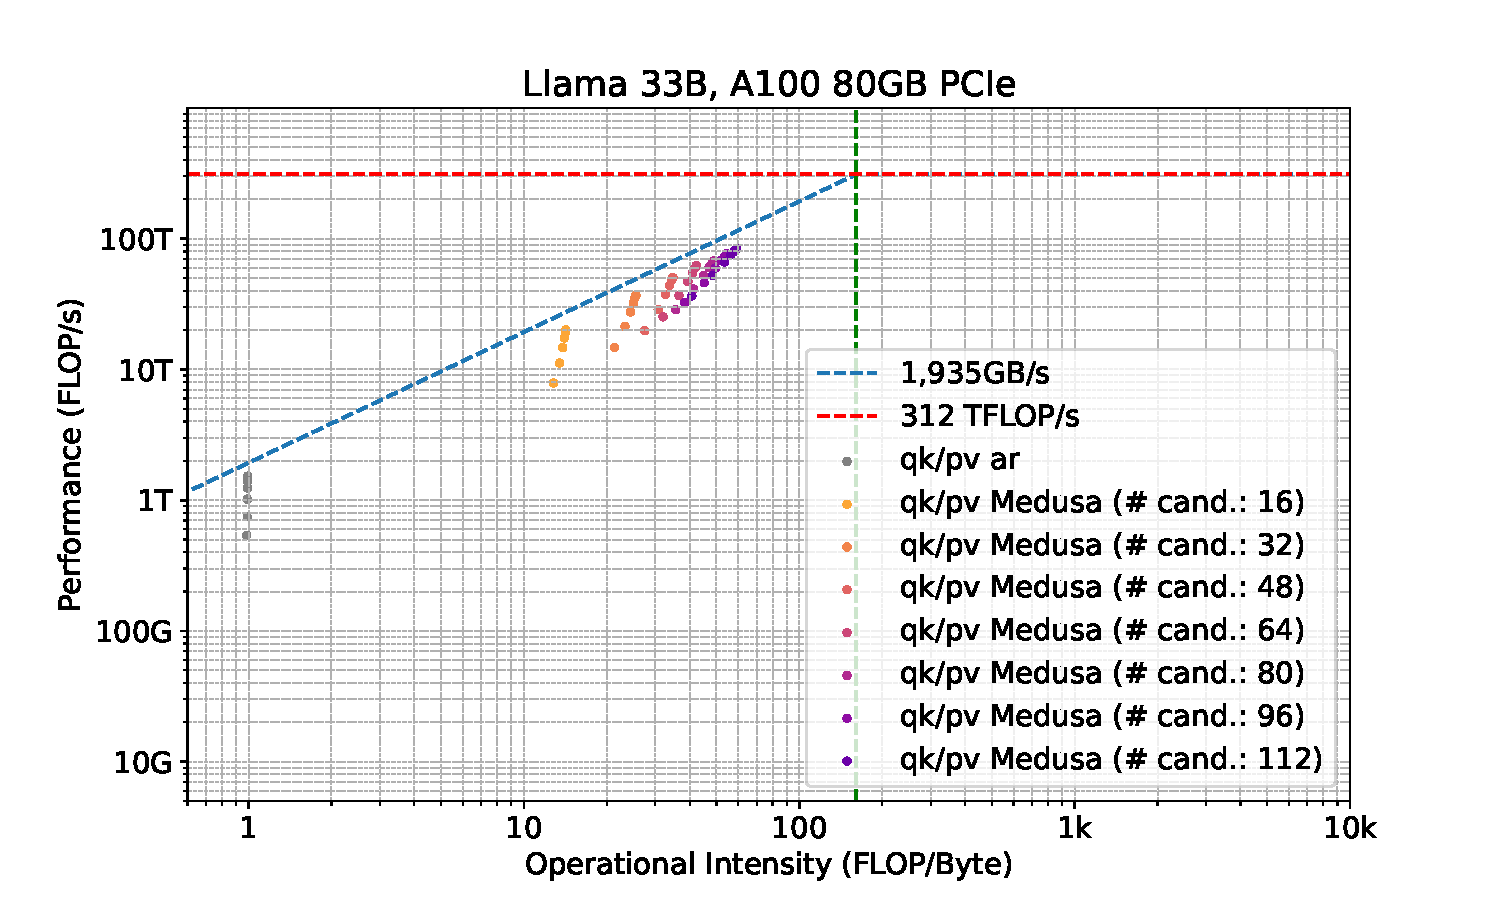
\includegraphics[width=0.8\textwidth]{llama33b-spec-bs16.pdf}
    \caption{FLOP/s vs. Operational Intensity of attention matrix multiplication with batch size 16.}
    \label{fig:llama33b-spec-bs16}
\end{figure}

\begin{figure}[h]
    \centering
    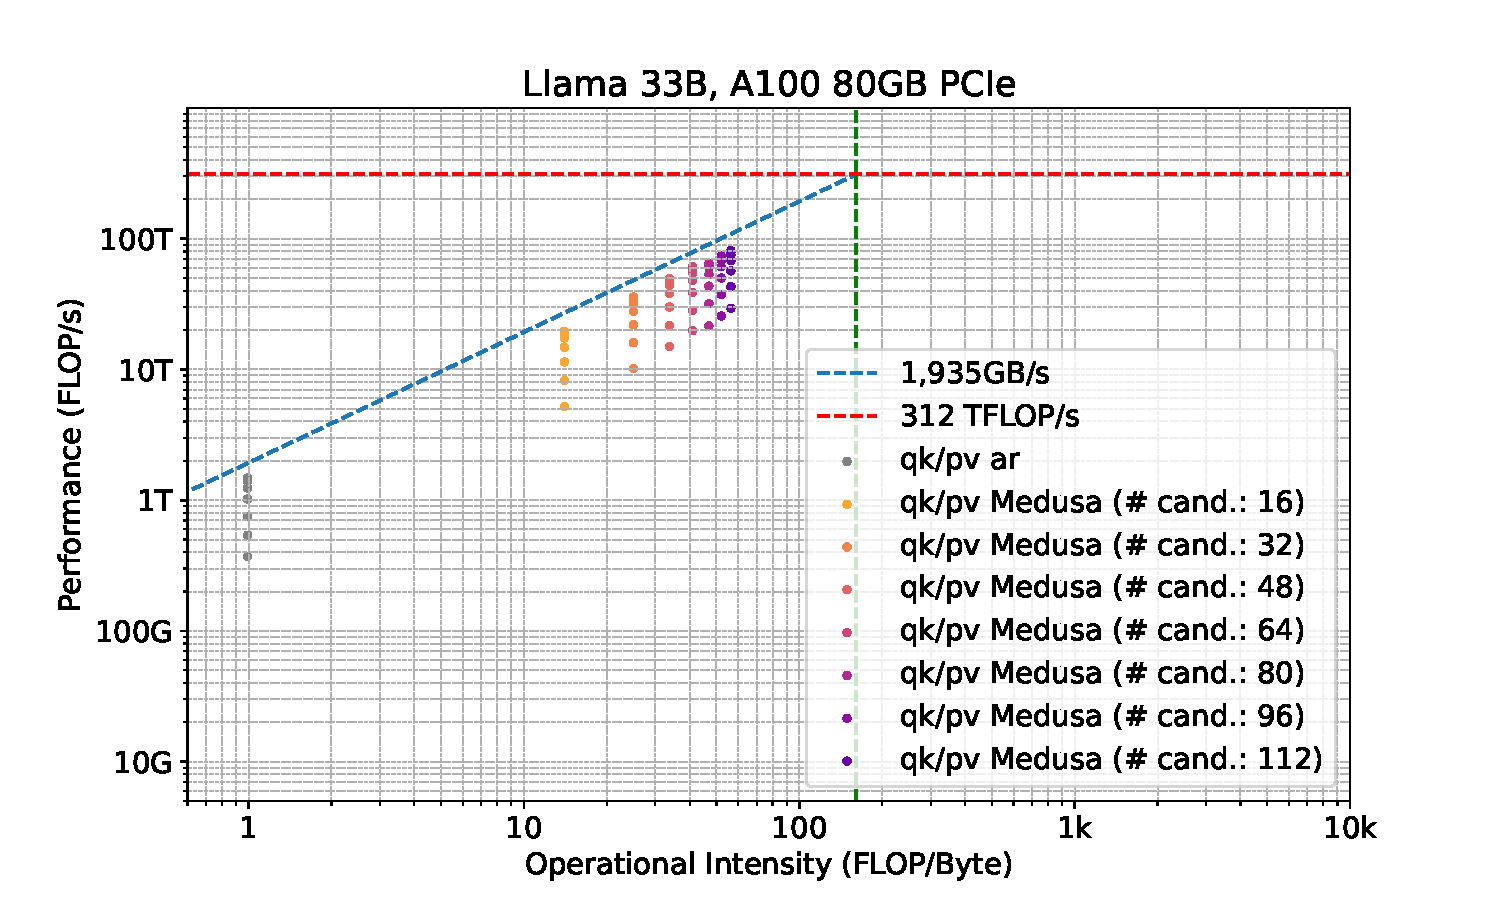
\includegraphics[width=0.8\textwidth]{llama33b-spec-seq1024.pdf}
    \caption{FLOP/s vs. Operational Intensity of attention matrix multiplication with sequence length 1024.}
    \label{fig:llama33b-spec-seq1024}
\end{figure}

\begin{figure}[h]
    \centering
    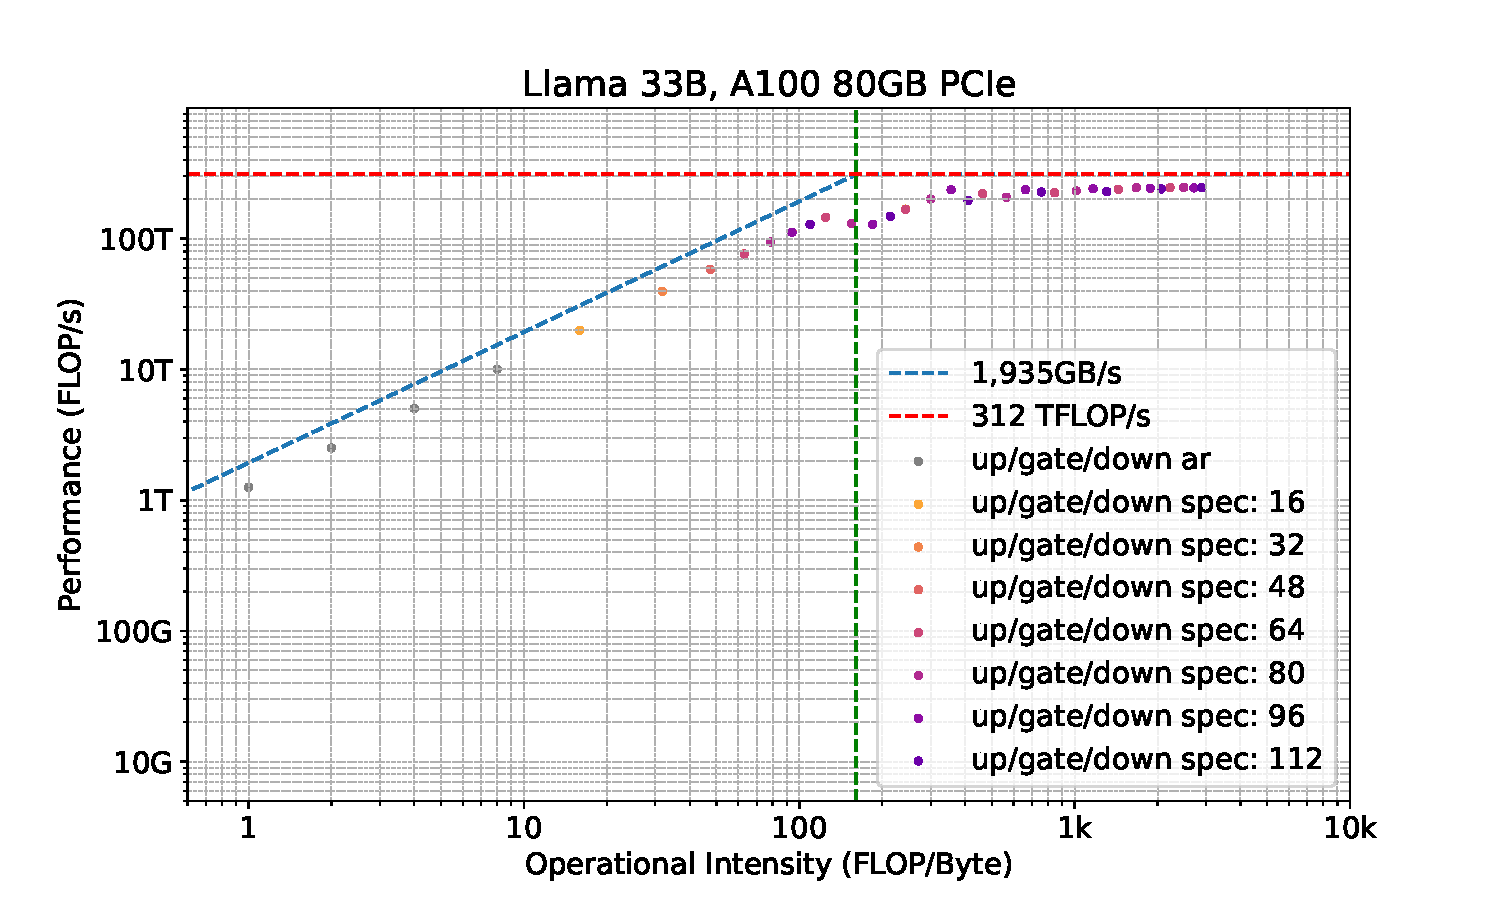
\includegraphics[width=0.8\textwidth]{llama33b-spec-mlp-bsall.pdf}
    \caption{FLOP/s vs. Operational Intensity of Linear layers.}
    \label{fig:llama33b-spec--mlp-bsall}
\end{figure}

\clearpage


\begin{table}[h]
\centering
\scriptsize
\begin{tabular}{lcccccccc}

\toprule
Seq. Length & \multicolumn{8}{c}{Number of Candidate Tokens} \\
\midrule
 & 1 & 16 & 32 & 48 & 64 & 80 & 96 & 112 \\
\midrule
128  & 0.54 \& 0.98 & 7.87 \& 12.8 & 14.73 \& 21.33 & 19.78 \& 27.43 & 25.25 \& 32.0 & 28.63 \& 35.56 & 32.58 \& 38.4 & 36.57 \& 40.73 \\
256  & 0.75 \& 0.99 & 11.2 \& 13.47 & 21.29 \& 23.27 & 28.69 \& 30.72 & 36.59 \& 36.57 & 41.2 \& 41.29 & 45.99 \& 45.18 & 52.33 \& 48.43 \\
512  & 1.02 \& 0.99 & 14.69 \& 13.84 & 27.47 \& 24.38 & 37.35 \& 32.68 & 47.09 \& 39.38 & 52.24 \& 44.91 & 59.55 \& 49.55 & 66.35 \& 53.49 \\
1024  & 1.24 \& 0.99 & 17.42 \& 14.03 & 32.15 \& 24.98 & 43.89 \& 33.76 & 54.8 \& 40.96 & 60.19 \& 46.97 & 68.28 \& 52.07 & 75.45 \& 56.44 \\
2048 & 1.39 \& 0.99 & 19.03 \& 14.12 & 35.05 \& 25.28 & 48.03 \& 34.32 & 59.66 \& 41.8 & 63.91 \& 48.08 & 72.83 \& 53.43 & 80.05 \& 58.04 \\
4096 & 1.48 \& 0.99 & 19.8 \& 14.17 & 36.59 \& 25.44 & 50.4 \& 34.61 & 62.29 \& 42.23 & 65.84 \& 48.65 & 74.86 \& 54.13 & 82.06 \& 58.87 \\
8192 & 1.53 \& 0.99 & 20.08 \& 14.2 & 36.89 \& 25.52 & 50.44 \& 34.76 & 62.11 \& 42.45 & 67.5 \& 48.94 & 76.97 \& 54.49 & 84.5 \& 59.3 \\
\bottomrule
\end{tabular}
\caption{
TFLOP/s \& Operational Intensity of attention matrix multiplication with batch size 16 for Llama 33B on an A100 80GB PCIe.}
\label{tab:llama33b-spec-bs16}
\end{table}


\begin{table}[h]
\centering
\scriptsize
\begin{tabular}{lcccccccc}
\toprule
Batch Size & \multicolumn{8}{c}{Number of Candidate Tokens} \\
\midrule
 & 1 & 16 & 32 & 48 & 64 & 80 & 96 & 112 \\
\midrule
1  & 0.37 \& 0.99 & 5.22 \& 14.03 & 10.15 \& 24.98 & 15.02 \& 33.76 & 19.79 \& 40.96 & 21.52 \& 46.97 & 25.65 \& 52.07 & 29.4 \& 56.44 \\
2  & 0.54 \& 0.99 & 8.25 \& 14.03 & 16.0 \& 24.98 & 21.62 \& 33.76 & 28.24 \& 40.96 & 31.84 \& 46.97 & 37.49 \& 52.07 & 43.04 \& 56.44 \\
4  & 0.75 \& 0.99 & 11.41 \& 14.03 & 21.97 \& 24.98 & 30.02 \& 33.76 & 38.71 \& 40.96 & 43.41 \& 46.97 & 50.06 \& 52.07 & 56.77 \& 56.44 \\
8  & 1.02 \& 0.99 & 14.78 \& 14.03 & 27.78 \& 24.98 & 38.09 \& 33.76 & 47.99 \& 40.96 & 53.32 \& 46.97 & 61.0 \& 52.07 & 68.11 \& 56.44 \\
16 & 1.24 \& 0.99 & 17.42 \& 14.03 & 32.15 \& 24.98 & 43.89 \& 33.76 & 54.8 \& 40.96 & 60.19 \& 46.97 & 68.28 \& 52.07 & 75.45 \& 56.44 \\
32 & 1.39 \& 0.99 & 18.89 \& 14.03 & 34.67 \& 24.98 & 47.57 \& 33.76 & 58.89 \& 40.96 & 63.61 \& 46.97 & 72.17 \& 52.07 & 79.21 \& 56.44 \\
64 & 1.48 \& 0.99 & 19.58 \& 14.03 & 35.87 \& 24.98 & 49.45 \& 33.76 & 61.13 \& 40.96 & 64.84 \& 46.97 & 73.73 \& 52.07 & 81.02 \& 56.44 \\

\bottomrule
\end{tabular}
\caption{
TFLOP/s \& Operational Intensity of attention matrix multiplication with sequence length 1024 for Llama 33B on an A100 80GB PCIe.}
\label{tab:llama33b-spec-seq1024}
\end{table}

\begin{table}[h]
\centering
\tiny
\begin{tabular}{lcccccccc}
\toprule
Batch Size & \multicolumn{8}{c}{Number of Candidate Tokens} \\
\midrule
 & 1 & 16 & 32 & 48 & 64 & 80 & 96 & 112 \\
\midrule
1  & 1.26 \& 1.0 & 19.95 \& 15.95 & 39.69 \& 31.79 & 58.4 \& 47.53 & 76.57 \& 63.17 & 94.4 \& 78.7 & 111.91 \& 94.14 & 128.64 \& 109.47 \\
2  & 2.51 \& 2.0 & 39.66 \& 31.79 & 76.53 \& 63.17 & 112.05 \& 94.14 & 145.73 \& 124.71 & 130.67 \& 154.89 & 129.1 \& 184.69 & 148.56 \& 214.12 \\
4  & 5.03 \& 4.0 & 76.44 \& 63.17 & 145.8 \& 124.71 & 128.85 \& 184.69 & 167.85 \& 243.17 & 201.19 \& 300.21 & 236.93 \& 355.85 & 195.91 \& 410.14 \\
8  & 10.06 \& 7.99 & 145.72 \& 124.71 & 168.26 \& 243.17 & 236.83 \& 355.85 & 221.11 \& 463.14 & 207.79 \& 565.44 & 236.95 \& 663.07 & 227.8 \& 756.36 \\
16 & 19.96 \& 15.95 & 168.35 \& 243.17 & 221.41 \& 463.14 & 237.5 \& 663.07 & 224.71 \& 845.59 & 232.49 \& 1012.87 & 241.12 \& 1166.74 & 229.25 \& 1308.76 \\
32 & 39.69 \& 31.79 & 221.74 \& 463.14 & 224.88 \& 845.59 & 241.33 \& 1166.74 & 239.02 \& 1440.25 & 245.83 \& 1675.97 & 243.55 \& 1881.24 & 240.33 \& 2061.59 \\
64 & 76.57 \& 63.17 & 225.19 \& 845.59 & 239.2 \& 1440.25 & 243.26 \& 1881.24 & 246.16 \& 2221.31 & 246.91 \& 2491.55 & 244.52 \& 2711.46 & 246.14 \& 2893.91 \\
\bottomrule
\end{tabular}
\caption{
TFLOP/s \& Operational Intensity of linear layers (up/gate/down) for Llama 33B on an A100 80GB PCIe.
}\label{tab:llama33b-spec--mlp-bsall}
\end{table}

\subsection{Predicting \ours Performance}

We further employ a straightforward analytical model \textcolor{black}{for} the acceleration rate. The ablation study results in Sec.~\ref{section:config of tree} indicate that the acceleration rate can be approximated by a simple logarithmic function. Using the results from Fig.~\ref{fig:sparse_acc}, we model the curve as $\texttt{acc\_rate} = 0.477 \log(\texttt{num\_candidate})$. We simulate the latency of one simplified block of the Llama-7B model (sequentially processing $XW_Q$, $XW_K$, $XW_V$, $QK^T$, $PV$, $XW_u$, $XW_g$, $XW_d$) by first fixing the batch size at 1 and the sequence length at 1024.
\textcolor{black}{
The candidate tokens are processed parallelly by constructing the tree attention described in Section~\ref{sec:tree_attention}. We omit the latency of the post-processing steps including verification and acceptance for \ours since they introduce marginal overhead.
}
Fig.~\ref{fig:llama7b-sim-bs1-seq1024} illustrates the simulated acceleration rate and speedup for different numbers of candidate tokens under these settings. As the number of candidate tokens increases, both the acceleration rate and speedup initially show improvements. However, beyond 64, the speedup starts to decline, indicating diminishing returns with further increases in candidate length. This aligns with the experimental results in Fig.~\ref{fig:sparse_speed} and suggests that there is an optimal range for the numbers of candidate tokens where \ours provides the most significant performance gains.

We plot the simulated speedup under different batch size settings with a fixed sequence length of 1024 in Fig.~\ref{fig:llama7b-sim-bs1-allbs}. The results indicate that when the batch size exceeds 32, the speedup decreases and may even have a negative effect. This occurs because the linear layers shift from being memory-bandwidth-bound to computationally bound.

We conduct another experiment using a batch size of 4 and different sequence lengths. As shown in Fig.~\ref{fig:llama7b-sim-allseq}, the optimal number of candidate tokens remains relatively consistent across different sequence lengths. However, as the sequence length increases, the overall performance decreases. This performance drop is primarily due to the overhead from attention matrix multiplication, while the linear layer computation remains constant \textcolor{black}{since the computation of linear layers is independent of the sequence length.}

Our simulations show that the optimal number of candidate tokens is key for model scaling with \ours, as benefits decrease beyond a certain range. Initially, increasing batch size improves performance through parallelism, but too large a batch size shifts linear layers from memory-bandwidth-bound to compute-bound, reducing speedup. Longer sequences increase attention matrix multiplication overhead, lowering performance, and emphasizing the need to optimize attention mechanisms. Effective model scaling requires balancing the number of candidate tokens, adjusting batch sizes to avoid compute-bound transitions, and enhancing attention mechanisms for longer sequences. These strategies ensure better resource utilization and higher performance, demonstrating the value of simulations in predicting performance and guiding acceleration strategy design.

\begin{figure}[h]
    \centering
    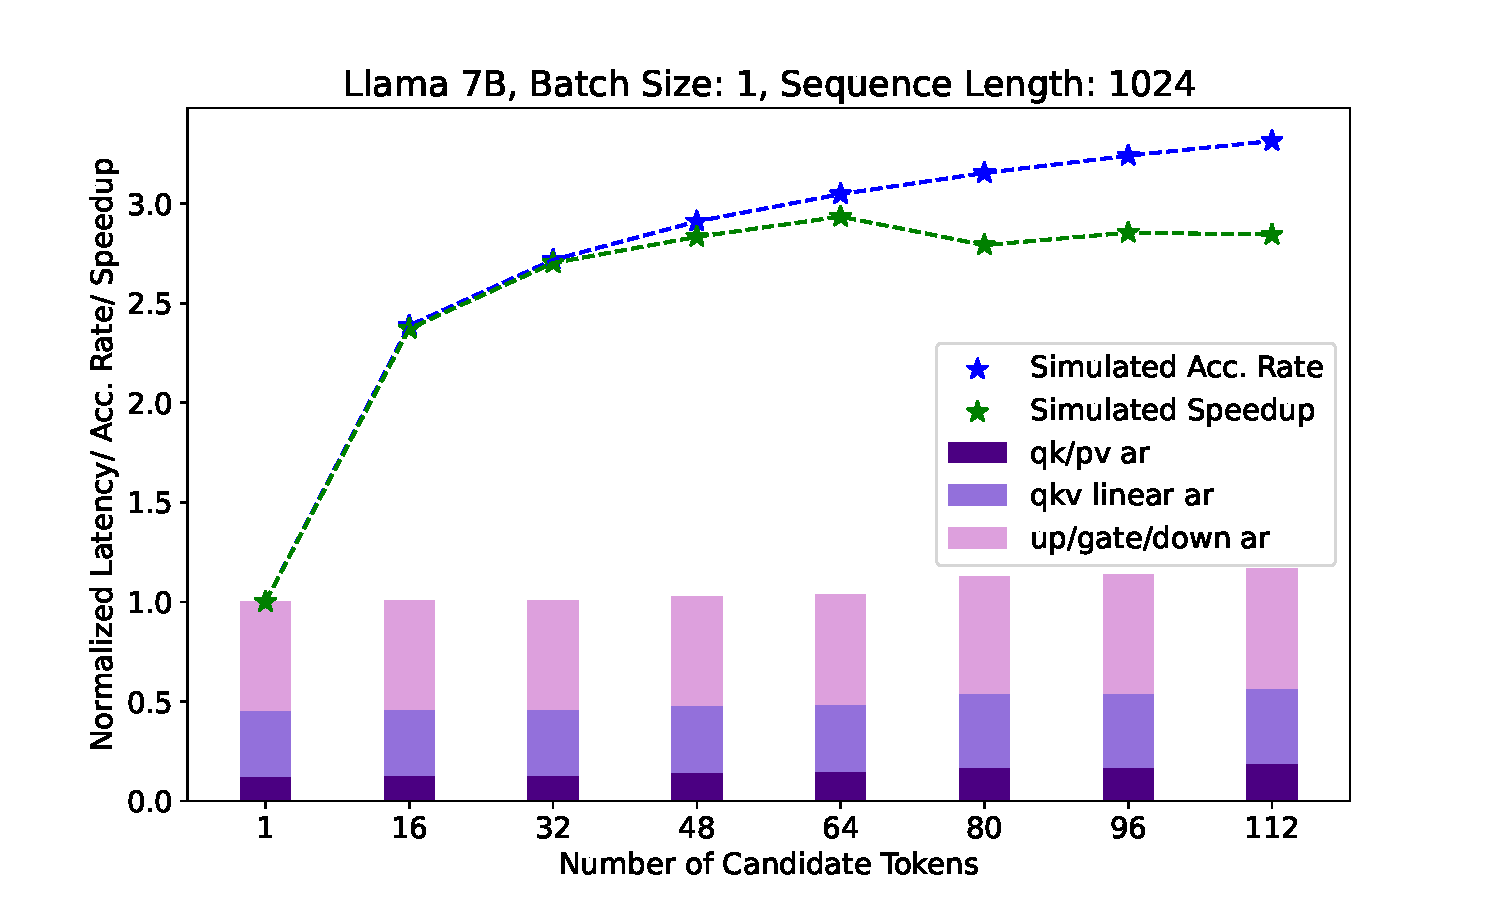
\includegraphics[width=0.8\textwidth]{llama7b-sim-bs1-seq1024.pdf}
    \caption{Simulated acceleration rate, speedup, and normalized latency ablation using different numbers of candidate tokens under the setting of batch size 1 and sequence length 1024 for Llama-7B on an A100 80GB PCIe.}
    \label{fig:llama7b-sim-bs1-seq1024}
\end{figure}

\begin{figure}[h]
    \centering
    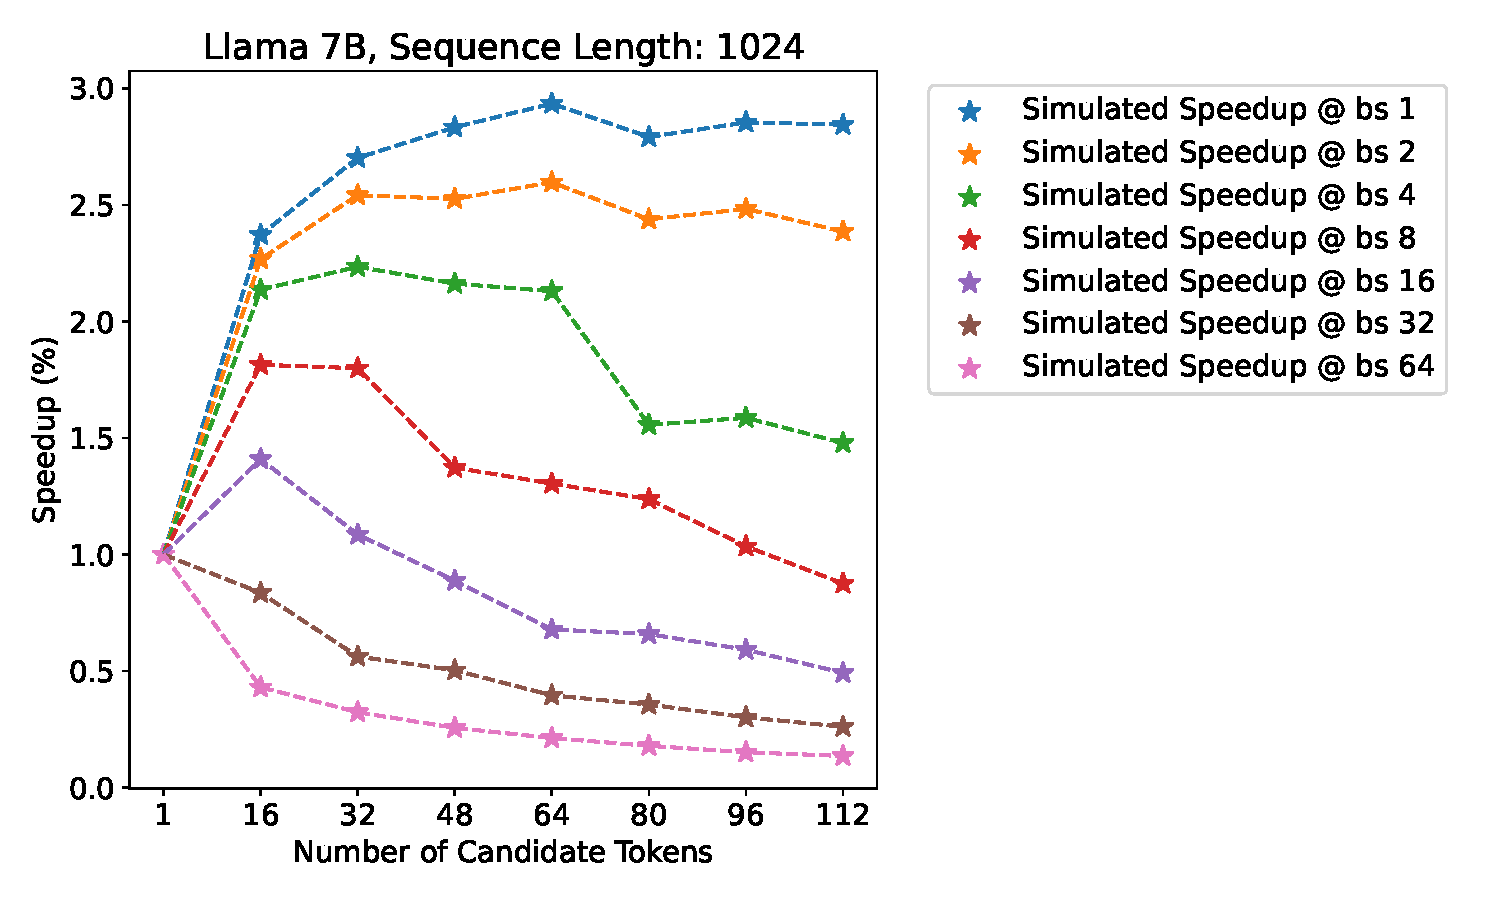
\includegraphics[width=0.8\textwidth]{llama7b-sim-allbs.pdf}
    \caption{Simulated speedup with sequence length 1024 for Llama-7B.}
    \label{fig:llama7b-sim-bs1-allbs}
\end{figure}

\begin{figure}[h]
    \centering
    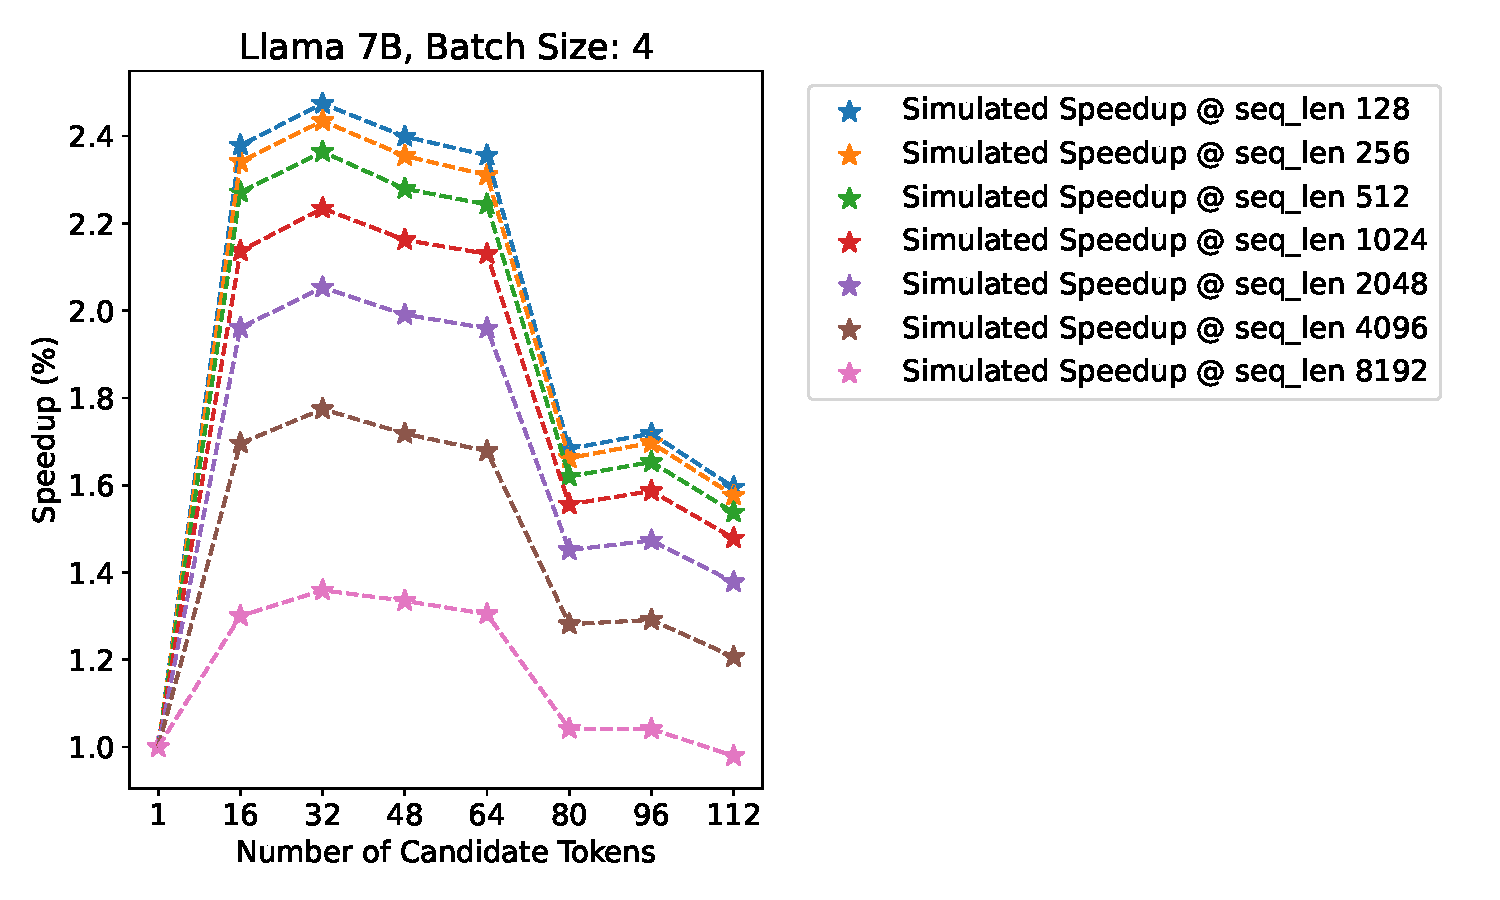
\includegraphics[width=0.8\textwidth]{llama7b-sim-allseq.pdf}
    \caption{Simulated speedup with batch size 4 for Llama-7B.}
    \label{fig:llama7b-sim-allseq}
\end{figure}
\end{document}